% Options for packages loaded elsewhere
\PassOptionsToPackage{unicode}{hyperref}
\PassOptionsToPackage{hyphens}{url}
\PassOptionsToPackage{dvipsnames,svgnames,x11names}{xcolor}
%
\documentclass[
  11pt,
]{article}

\usepackage{amsmath,amssymb}
\usepackage{setspace}
\usepackage{iftex}
\ifPDFTeX
  \usepackage[T1]{fontenc}
  \usepackage[utf8]{inputenc}
  \usepackage{textcomp} % provide euro and other symbols
\else % if luatex or xetex
  \usepackage{unicode-math}
  \defaultfontfeatures{Scale=MatchLowercase}
  \defaultfontfeatures[\rmfamily]{Ligatures=TeX,Scale=1}
\fi
\usepackage{lmodern}
\ifPDFTeX\else  
    % xetex/luatex font selection
  \setmainfont[]{Arial}
  \setmonofont[]{DejaVu Sans Mono}
\fi
% Use upquote if available, for straight quotes in verbatim environments
\IfFileExists{upquote.sty}{\usepackage{upquote}}{}
\IfFileExists{microtype.sty}{% use microtype if available
  \usepackage[]{microtype}
  \UseMicrotypeSet[protrusion]{basicmath} % disable protrusion for tt fonts
}{}
\makeatletter
\@ifundefined{KOMAClassName}{% if non-KOMA class
  \IfFileExists{parskip.sty}{%
    \usepackage{parskip}
  }{% else
    \setlength{\parindent}{0pt}
    \setlength{\parskip}{6pt plus 2pt minus 1pt}}
}{% if KOMA class
  \KOMAoptions{parskip=half}}
\makeatother
\usepackage{xcolor}
\usepackage[lmargin=0.8in,rmargin=0.8in,tmargin=0.8in,bmargin=0.8in]{geometry}
\setlength{\emergencystretch}{3em} % prevent overfull lines
\setcounter{secnumdepth}{-\maxdimen} % remove section numbering
% Make \paragraph and \subparagraph free-standing
\ifx\paragraph\undefined\else
  \let\oldparagraph\paragraph
  \renewcommand{\paragraph}[1]{\oldparagraph{#1}\mbox{}}
\fi
\ifx\subparagraph\undefined\else
  \let\oldsubparagraph\subparagraph
  \renewcommand{\subparagraph}[1]{\oldsubparagraph{#1}\mbox{}}
\fi


\providecommand{\tightlist}{%
  \setlength{\itemsep}{0pt}\setlength{\parskip}{0pt}}\usepackage{longtable,booktabs,array}
\usepackage{calc} % for calculating minipage widths
% Correct order of tables after \paragraph or \subparagraph
\usepackage{etoolbox}
\makeatletter
\patchcmd\longtable{\par}{\if@noskipsec\mbox{}\fi\par}{}{}
\makeatother
% Allow footnotes in longtable head/foot
\IfFileExists{footnotehyper.sty}{\usepackage{footnotehyper}}{\usepackage{footnote}}
\makesavenoteenv{longtable}
\usepackage{graphicx}
\makeatletter
\def\maxwidth{\ifdim\Gin@nat@width>\linewidth\linewidth\else\Gin@nat@width\fi}
\def\maxheight{\ifdim\Gin@nat@height>\textheight\textheight\else\Gin@nat@height\fi}
\makeatother
% Scale images if necessary, so that they will not overflow the page
% margins by default, and it is still possible to overwrite the defaults
% using explicit options in \includegraphics[width, height, ...]{}
\setkeys{Gin}{width=\maxwidth,height=\maxheight,keepaspectratio}
% Set default figure placement to htbp
\makeatletter
\def\fps@figure{htbp}
\makeatother
% definitions for citeproc citations
\NewDocumentCommand\citeproctext{}{}
\NewDocumentCommand\citeproc{mm}{%
  \begingroup\def\citeproctext{#2}\cite{#1}\endgroup}
\makeatletter
 % allow citations to break across lines
 \let\@cite@ofmt\@firstofone
 % avoid brackets around text for \cite:
 \def\@biblabel#1{}
 \def\@cite#1#2{{#1\if@tempswa , #2\fi}}
\makeatother
\newlength{\cslhangindent}
\setlength{\cslhangindent}{1.5em}
\newlength{\csllabelwidth}
\setlength{\csllabelwidth}{3em}
\newenvironment{CSLReferences}[2] % #1 hanging-indent, #2 entry-spacing
 {\begin{list}{}{%
  \setlength{\itemindent}{0pt}
  \setlength{\leftmargin}{0pt}
  \setlength{\parsep}{0pt}
  % turn on hanging indent if param 1 is 1
  \ifodd #1
   \setlength{\leftmargin}{\cslhangindent}
   \setlength{\itemindent}{-1\cslhangindent}
  \fi
  % set entry spacing
  \setlength{\itemsep}{#2\baselineskip}}}
 {\end{list}}
\usepackage{calc}
\newcommand{\CSLBlock}[1]{\hfill\break\parbox[t]{\linewidth}{\strut\ignorespaces#1\strut}}
\newcommand{\CSLLeftMargin}[1]{\parbox[t]{\csllabelwidth}{\strut#1\strut}}
\newcommand{\CSLRightInline}[1]{\parbox[t]{\linewidth - \csllabelwidth}{\strut#1\strut}}
\newcommand{\CSLIndent}[1]{\hspace{\cslhangindent}#1}

\usepackage{lineno}
\makeatletter
\@ifpackageloaded{caption}{}{\usepackage{caption}}
\AtBeginDocument{%
\ifdefined\contentsname
  \renewcommand*\contentsname{Table of contents}
\else
  \newcommand\contentsname{Table of contents}
\fi
\ifdefined\listfigurename
  \renewcommand*\listfigurename{List of Figures}
\else
  \newcommand\listfigurename{List of Figures}
\fi
\ifdefined\listtablename
  \renewcommand*\listtablename{List of Tables}
\else
  \newcommand\listtablename{List of Tables}
\fi
\ifdefined\figurename
  \renewcommand*\figurename{Figure}
\else
  \newcommand\figurename{Figure}
\fi
\ifdefined\tablename
  \renewcommand*\tablename{Table}
\else
  \newcommand\tablename{Table}
\fi
}
\@ifpackageloaded{float}{}{\usepackage{float}}
\floatstyle{ruled}
\@ifundefined{c@chapter}{\newfloat{codelisting}{h}{lop}}{\newfloat{codelisting}{h}{lop}[chapter]}
\floatname{codelisting}{Listing}
\newcommand*\listoflistings{\listof{codelisting}{List of Listings}}
\makeatother
\makeatletter
\makeatother
\makeatletter
\@ifpackageloaded{caption}{}{\usepackage{caption}}
\@ifpackageloaded{subcaption}{}{\usepackage{subcaption}}
\makeatother
\ifLuaTeX
  \usepackage{selnolig}  % disable illegal ligatures
\fi
\usepackage{bookmark}

\IfFileExists{xurl.sty}{\usepackage{xurl}}{} % add URL line breaks if available
\urlstyle{same} % disable monospaced font for URLs
\hypersetup{
  pdftitle={Whole-body connectome of a segmented annelid larva},
  colorlinks=true,
  linkcolor={blue},
  filecolor={Maroon},
  citecolor={Blue},
  urlcolor={Blue},
  pdfcreator={LaTeX via pandoc}}

\title{Whole-body connectome of a segmented annelid larva}
\author{}
\date{}

\begin{document}
\maketitle

\linenumbers

\setstretch{1.2}
\hfill\break

Gáspár Jékely\textsuperscript{1,2,*} , Sanja Jasek\textsuperscript{1,2},
Martin Gühmann\textsuperscript{3}, Luis Alberto Bezares
Calderón\textsuperscript{2}, Elizabeth A. Williams\textsuperscript{4},
Réza Shahidi\textsuperscript{5}\\

\textsuperscript{1}Heidelberg University, Centre for Organismal Studies
(COS), 69120 Heidelberg, Germany\\
\textsuperscript{2}Living Systems Institute, University of Exeter,
Exeter, EX4 4QD, United Kingdom\\
\textsuperscript{3}School of Biological Sciences, University of Bristol,
Bristol, United Kingdom\\
\textsuperscript{4}BioSciences, University of Exeter, Stocker Road,
Exeter EX4 4QD, Exeter, United Kingdom\\
\textsuperscript{5}Electron Microscopy Core Facility (EMCF), University
of Heidelberg, 69120 Heidelberg, Germany\\
\textsuperscript{*}Correspondence: gaspar.jekely@cos.uni-heidelberg.de

\section{Abstract}\label{abstract}

Nervous systems coordinate effectors across the body during movements.
We know little about the cellular-level structure of synaptic circuits
for such body-wide control. Here we describe the whole-body synaptic
connectome of a segmented larva of the marine annelid \emph{Platynereis
dumerilii}. We reconstructed and annotated over 9,000 neuronal and
non-neuronal cells in a whole-body serial electron microscopy dataset.
Differentiated cells were classified into 202 neuronal and 92
non-neuronal cell types. We analyse modularity, multisensory
integration, left-right and intersegmental connectivity and motor
circuits for ciliated cells, glands, pigment cells and muscles. We
identify several segment-specific cell types, demonstrating the
heteromery of the annelid larval trunk. At the same time, segmentally
repeated cell types across the head, the trunk segments and the pygidium
suggest the serial homology of all segmental body regions. We also
report descending and ascending pathways, peptidergic circuits and a
multi-modal mechanosensory girdle. Our work provides the basis for
understanding whole-body coordination in an entire segmented animal.

\section{Introduction}\label{introduction}

Nervous systems coordinate behaviour, physiology and development through
synaptic and neuroendocrine signalling. Signalling occurs specifically
between groups of cells, organised into multilayered networks with
precise synaptic and neuromodulatory connectivity (Bentley et al.,
2016). Mapping such synaptic and chemical networks in blocks of neural
tissue is the central aim of cellular-level connectomics (Deng et al.,
2019; Helmstaedter, 2013; Morgan and Lichtman, 2013; Williams et al.,
2017). For synaptic networks, connectomics requires volume imaging by
serial electron microscopy (serial EM) (Schlegel et al., 2017). The
comprehensive analysis of whole-body coordination of actions by synaptic
circuits would benefit from the cellular-level mapping of entire nervous
and effector systems. Whole-animal synaptic connectomes have so far only
been described for the nematode \emph{Caenorhabditis elegans} (Cook et
al., 2019; White et al., 1986) and the tadpole larva of the ascidian
\emph{Ciona intestinalis} (Ryan et al., 2016). Circuits spanning the
entire central nervous system (CNS) have also been reconstructed in the
larval CNS of the fruit fly \emph{Drosophila melanogaster}
(Carreira-Rosario et al., 2018; Miroschnikow et al., 2018; Ohyama et
al., 2015) and in the three-day-old larva of the annelid
\emph{Platynereis dumerilii} (Bezares-Calderón et al., 2018; Randel et
al., 2015; Verasztó et al., 2017). Recently, whole-brain connectomics
has become possible in the larval and adult fly brain (Franconville et
al., 2018; Winding et al., 2023; Zheng et al., 2018).

Here we report the complete synaptic connectome and the cell-type
complement of a three-day-old larva (nectochaete stage) of the marine
annelid \emph{Platynereis dumerilii}. This larval stage has three trunk
segments, adult and larval eyes, segmental ciliary bands and a
well-developed somatic musculature (Jasek et al., 2022). The larvae show
several behaviours, including visual phototaxis (Randel et al., 2014),
UV avoidance (Verasztó et al., 2018), a startle response
(Bezares-Calderón et al., 2018) and coordinated ciliary activity
(Verasztó et al., 2017). Three-day-old larvae do not yet have sensory
palps and other sensory appendages (cirri), they do not feed and lack
visceral muscles and an enteric nervous system (Brunet et al., 2016;
Williams et al., 2015).

In \emph{Platynereis} larvae, it has been possible to integrate
behaviour with synapse-level maps, transgenic labelling of individual
neurons, activity imaging and gene knockouts (Bezares-Calderón et al.,
2018; Jokura et al., 2023; Verasztó et al., 2018, 2017).
Cellular-resolution gene expression atlases have also been developed for
different larval stages. These can increasingly be integrated with
single-cell transcriptomic atlases and synaptic circuit maps (Achim et
al., 2015; Vergara et al., 2021; Vergara et al., 2017; Williams et al.,
2017). The registration of a gene expression atlas to a whole-body
low-resolution EM volume in the six-day-old \emph{Platynereis} larva has
also been reported (Vergara et al., 2021).

We previously reported synaptic connectomes for several whole-body
circuits from a transmission EM volume of a three-day-old larva (Randel
et al., 2015). These include the visual, startle, ciliomotor, nuchal
organ, and neurosecretory systems (Bezares-Calderón et al., 2018; Randel
et al., 2015; Shahidi et al., 2015; Verasztó et al., 2018, 2017;
Williams et al., 2017). Here, we report the complete synaptic connectome
and the cell-type complement from the same volume of a three-day-old
\emph{Platynereis} larva. Recently we also reported the desmosomal
connectome and motoneuron innervation of the somatic musculature (Jasek
et al., 2022) and a preprint of a preliminary analysis of the synaptic
connectome (Verasztó et al., 2020) that this work supersedes. The full
connectome reconstruction has now allowed us to uncover several new
circuits and to consider all circuits in a whole-body context. We also
found several neurons that span the entire length of the larva,
highlighting the strength of a whole-body dataset. These cells and their
circuits allow us to generate hypotheses on how whole-body coordination
may be achieved by the larval nervous system. The connectome also allows
us to address long-standing hypotheses about the origin of the segmented
annelid body-plan and explore patterns of circuit evolution.

\section{Results}\label{results}

\subsubsection{\texorpdfstring{Serial EM reconstruction of a
\emph{Platynereis}
larva}{Serial EM reconstruction of a Platynereis larva}}\label{serial-em-reconstruction-of-a-platynereis-larva}

We traced and annotated all cells in a previously reported volume EM
dataset of a three-day-old (72 hours post fertilisation (hpf))
\emph{Platynereis} larva (Randel et al., 2015) (Figure 1A, Figure
1---figure supplement 1). The dataset consists of 4,846 layers of 40 nm
thin sections scanned by transmission electron microscopy (TEM). The
sections span the entire body of the larva. In the volume, we identified
9,162 cells with a soma.

We skeletonised cells containing projections or having an elongated
morphology including muscle cells, glia and neurons (Figure 1C, D).
During skeletonisation, interconnected nodes are placed in the neurite
cross-section profiles of the same neuron across layers. The skeletons
are grown until all branches of a neuron have been traced. The
individual nodes can be tagged and the skeletons named and multiply
annotated. For all neuronal skeletons, we also identified and marked
synaptic sites as connectors. Connectors link a node of a presynaptic
skeleton to a node of a postsynaptic skeleton partner. Synapses were
recognised as presynaptic vesicle clusters at the membrane with no
postsynaptic specialisations, as previously described (Randel et al.,
2014). Synapses are monoadic, connecting one presynaptic neuron to one
postsynaptic cell. Querying all skeletons and synaptic connectors
allowed us to derive the synaptic connectome (Figure 1, Figure 2). We
did not identify any gap junctions.

The skeletons across the volume comprised 5,661,050 nodes and had 28,717
presynaptic and 27,538 postsynaptic sites. We could not attach 15,020
fragments (896,428 nodes) to a skeleton with a soma. These fragments
contained 4,122 presynaptic and 5,304 postsynaptic sites. Most of the
fragments represent short skeletons of twigs (median length 1.04
µm)(Figure 1---figure supplement 2B) that could not be traced across
gaps or low-quality layers. Overall, 15.8\% of all nodes, 14.4\% of
presynaptic, and 19.3\% of postsynaptic sites are on fragments and not
assigned to a cell with a soma.

\begin{figure}[H]

{\centering 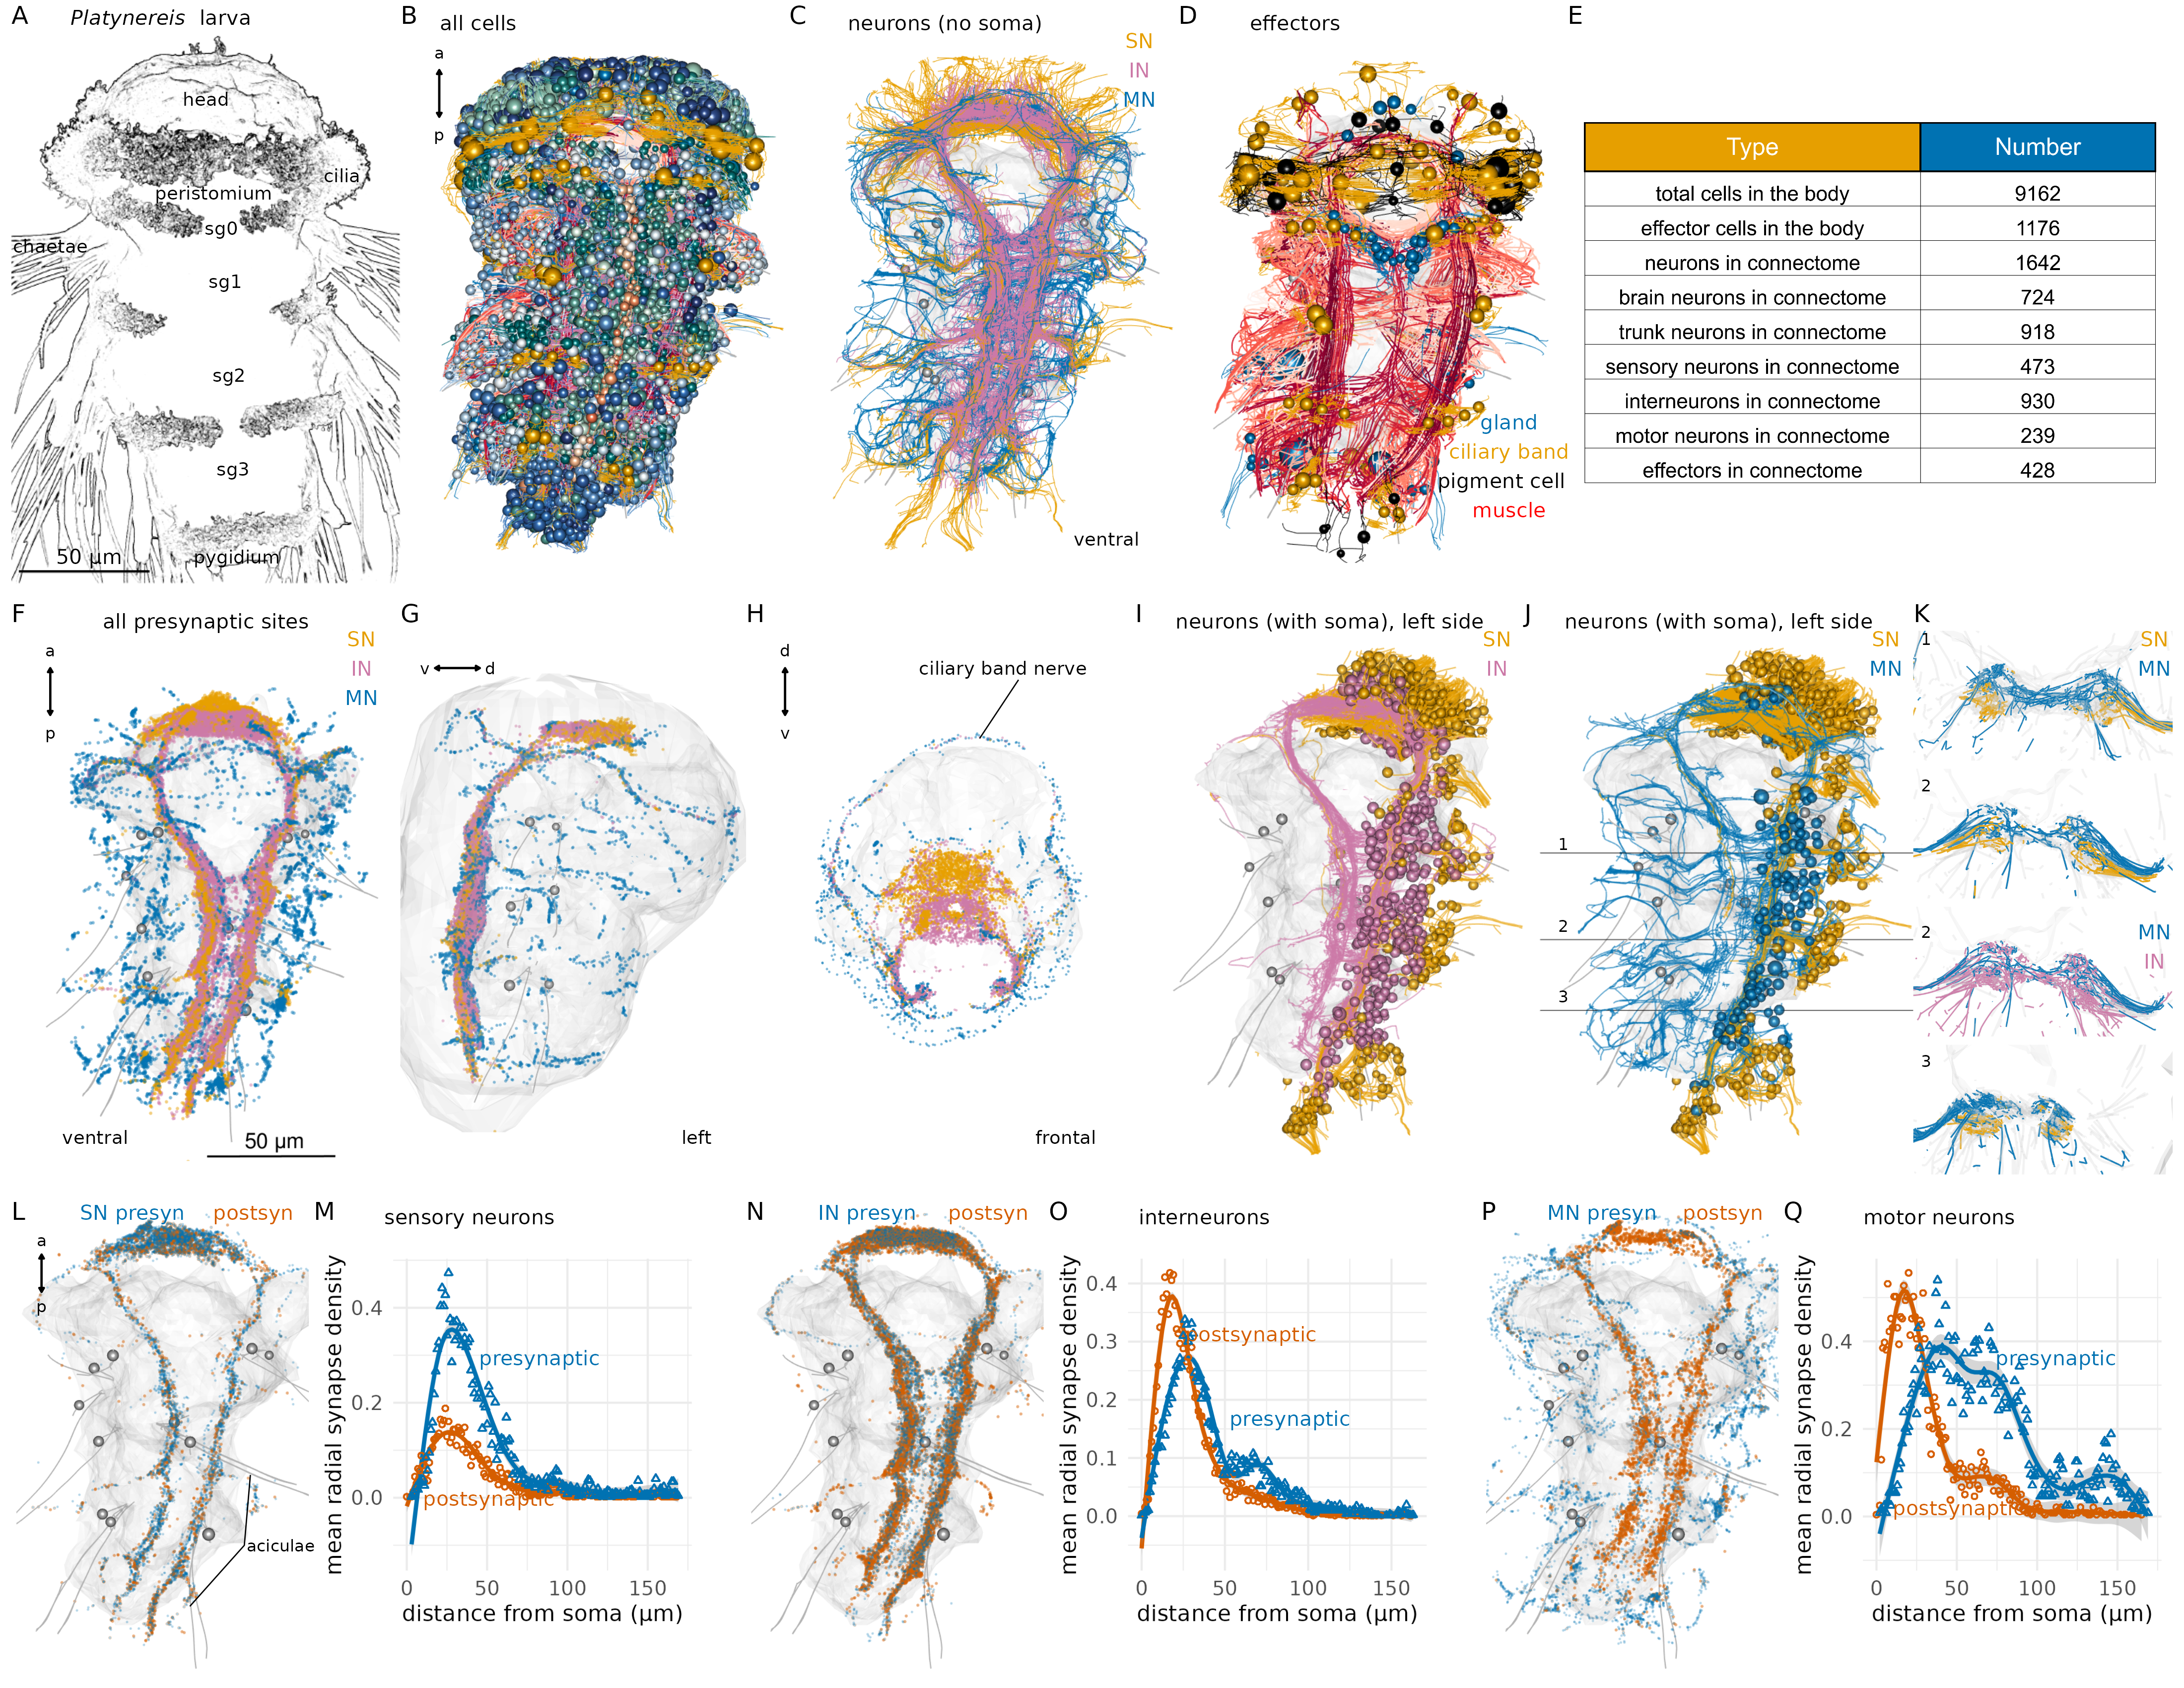
\includegraphics[width=1\textwidth,height=\textheight]{Figures/Figure1.png}

}

\caption{\textbf{Figure 1. Overview of nervous-system anatomy in the
three-day-old \emph{Platynereis} larva.} (A) Stylised scanning electron
microscopy image of a three-day-old segmented \emph{Platynereis} larva.
(B) Morphological rendering of all cells in the EM volume. Spheres
represent the position of cell somas. (C) Neurite processes of all
neurons in the larva coloured by neuron type (ventral view). Soma are
not shown. (D) All effector cells in the larva, including ciliated cells
(yellow), glands (grey) and muscles (red). Spheres indicate cell soma
(not shown for muscle cells) (E) Summary of cell numbers of different
categories in the larva. (F-H) All presynaptic sites coloured by neuron
type shown in (F) ventral, lateral (G), and frontal (H) views. (I)
Morphological rendering of all sensory and interneurons on the left side
of the larva. (J) Morphological rendering of all sensory and motor
neurons on the left side of the larva. Horizontal lines indicate the
position of the cross-sections in (K). (K) Cross-section view of
sensory, inter- and motor neuron projections in the ventral nerve cord
neuropil. Cross-sections at three antero-posterior positions are shown.
Numbers indicate the position of the cross-sections as marked in (J).
(L) Position of presynaptic and postsynaptic sites on all sensory
neurons of the connectome. (M) Mean radial synapse density (radius: 1000
nm, centre: soma) of incoming and outgoing synapses in sensory neurons.
(N) Position of presynaptic and postsynaptic sites on all interneurons
of the connectome. (O) Mean radial synapse density (radius: 1000 nm,
centre: soma) of incoming and outgoing synapses in interneurons. (P)
Position of presynaptic and postsynaptic sites on all motor neurons of
the connectome. (Q) Mean radial synapse density (radius: 1000 nm,
centre: soma) of incoming and outgoing synapses in motor neurons. In all
anatomical renderings, the outline of the yolk is shown in grey. In (G),
the body outline is also shown. Aciculae and chaetae are also shown in
grey as segmental markers. Abbreviations: SN, sensory neuron; IN,
interneuron; MN, motor neuron, sg0-3, segments 0-3. Figure 1---source
data 1. Source data for panels M, O, Q.}

\end{figure}%

\subsubsection{Neuroanatomy and
neuropils}\label{neuroanatomy-and-neuropils}

The \emph{Platynereis} larval nervous system is subdivided into an
anterior brain and a rope-ladder-like paired ventral nerve cord (VNC).
The brain and VNC are connected by circumesophageal connectives (Figure
1C, F-H). The trunk has five segments, an anterior cryptic segment
(segment 0)(Steinmetz et al., 2011), three main segments (segments 1-3)
with parapodia, and a posterior pygidium (Figure 1A, B).

Morphological rendering of all synapses in the volume highlights the
overall organisation of neuropils and motor nerves. In the brain,
sensory, inter- and motoneurons synapse in partly overlapping regions,
with sensory neuron synapses occurring more anteriorly. In the head as
well as the VNC, motor synapses mark the periphery (Figure 1F-H).

The VNC also has an organised neuropil architecture. Sensory neurons in
the trunk only have ipsilateral projections that concentrate in two
ventro-lateral bundles in the VNC (Figure 1I-K). Interneurons have
either ipsi- or contralateral projections that remain in the VNC
neuropil and also concentrate ventrally in the VNC (Figure 1K).
Motoneurons can have ipsilateral and contralateral projections and are
the only neuron class with peripheral afferent projections (Figure 1J).
Motor nerves concentrate dorsally in the VNC (Figure 1K), close to the
basal lamina and mesodermal muscles.

Neurons have a median cable length of 97.1 µm (sensory neurons: 101.6
µm; interneurons: 87.77 µm, motoneurons: 139.8 µm)(Figure 1---figure
supplement 2A) and the largest neurons (Ser-tr1 and Loop) a cable length
of 1.2-1.7 mm.

Neurons have a median of 8 outgoing (presynpatic) and 6 incoming
(postsynaptic) synaptic sites with the largest neurons (MC, Ser-tr1,
Loop) with over 300 outgoing synapses (Figure 1---figure supplement 2).

The relative ratio of incoming and outgoing sites distinguishes sensory,
inter- and motoneurons, with sensory neurons having relatively more
outgoing synapses (Figure 1---figure supplement 2E).

The number of outgoing and incoming synaptic sites and skeleton segments
scales with the total cable length of skeletons with Pearson's
correlation coefficients \textgreater0.7 (Figure 1---figure supplement
2F-H).

Most neuronal trees are unipolar and not highly branched (\textless100
segments; Figure 1---figure supplement 2H). Neurons in general do not
have primary cilia. Sensory neurons are bipolar with an axon and a
sensory dendrite bearing zero to five sensory cilia at its proximal tip,
showing different sensory specialisations (Bezares-Calderón et al.,
2018; Williams et al., 2017). Interneurons are unipolar or
pseudo-unipolar. Ciliomotor neurons have two motor axons emanating from
the soma (Verasztó et al., 2017), other motoneurons are unipolar.

\subsubsection{Derivation and network analysis of the whole-body
synaptic
connectome}\label{derivation-and-network-analysis-of-the-whole-body-synaptic-connectome}

To define a whole-body synaptic connectome for the larva, we
comprehensively identified synapses by traversing the volume and each
skeleton multiple times (32,381 synapses). Synapses were connected to
the pre- and postsynaptic skeletons (one to one, as synapses are
monoadic). We then retrieved all synapses and their pre- and
postsynaptic skeletons and derived a graph (6,725 graph nodes or
vertices). From this graph, nodes with less than three connections were
removed. The final synaptic connectome contains 2,675 nodes (including
467 fragments) connected by 14,066 directed edges formed by 26,881
in-graph synapses (Figure 2). The connectome is a sparsely-connected
network with a graph density of 0.00197.

In the graph, the majority of source nodes (nodes with only outgoing
edges) are sensory neurons, sink nodes (nodes with only incoming edges)
are mostly effector cells (Figure 2---figure supplement 1). The nodes
with the highest degree included ciliomotor neurons (e.g.~Loop,
Ser-tr1)(Bezares-Calderón et al., 2018; Verasztó et al., 2017), the
sensory-motoneuron pygPBunp (Verasztó et al., 2017), and the motoneurons
of exocrine glands (MNspinning, see below). Some of the strongest edges
(highest number of synapses) were between the pigment-cell motoneuron
cioMNcover and prototroch pigment cells, MNspinning and exocrine glands,
and the previously described MC cell and ciliated cells (Verasztó et
al., 2017).

To identify more strongly connected subgraphs within the connectome, we
used community detection with the Leiden algorithm (Traag et al., 2019).
This analysis combined with force-field-based clustering highlighted
several modules (Figures 2). Nodes in a module are more strongly
interconnected than to nodes in other modules (Figure 2---figure
supplement 3). We named the modules based on their primary effector
organs or other dominant anatomical characters. We would like to note
that this analysis can recover varying numbers of modules depending on
the resolution parameter (Figure 2---figure supplement 2C). The selected
resolution parameter subdivides the network into communities that we
think best represent functional units.

The modules include the anterior neurosecretory centre, the mushroom
bodies, the visual circuit, a network of ciliomotor neurons, a module
innervating head pigment cells, a left and right mechanosensory module
providing input to muscles and segmental exocrine glands, a module for
trunk postural control, and five muscle-motor modules (Figures 2).

The modules contain neurons that project to distinct neuropil domains
(Figures 2---figure supplement 5) and likely correspond to functional
units. The visual module contains neurons of the eyes and primary visual
neuropil (PRC, IN1, INint, INton) previously shown to mediate visual
phototaxis (Randel et al., 2014). The ciliomotor module contains ciliary
band cells and functionally related neurons that show coordinated
activity and drive ciliary closures and beating (Ser-tr1, Loop, MNant)
(Verasztó et al., 2017). The anterior neurosecretory centre includes
anterior and dorsal sensory neurons, the ciliary photoreceptors and
their postsynaptic circuit including the INRGWa and INNOS interneurons
as well as the Ser-h1 and MC ciliomotors with their prototroch targets.
Neurons in this module mediate barotaxis and UV avoidance (Calderón et
al., 2023; Jokura et al., 2023; Verasztó et al., 2018).

The modules are also interconnected among themselves suggesting
crosstalk. Most sensory neurons occur in the visual, the two
mechanosensory, the mushroom body and the anterior neurosecretory
modules (Figure 2---figure supplement 1J). In a Sankey network diagram
representing information flow, these modules are upstream of the
motor-dominated pigmentmotor, ciliomotor, and musclemotor modules
(Figure 2---figure supplement 2B).

\begin{figure}[H]

{\centering 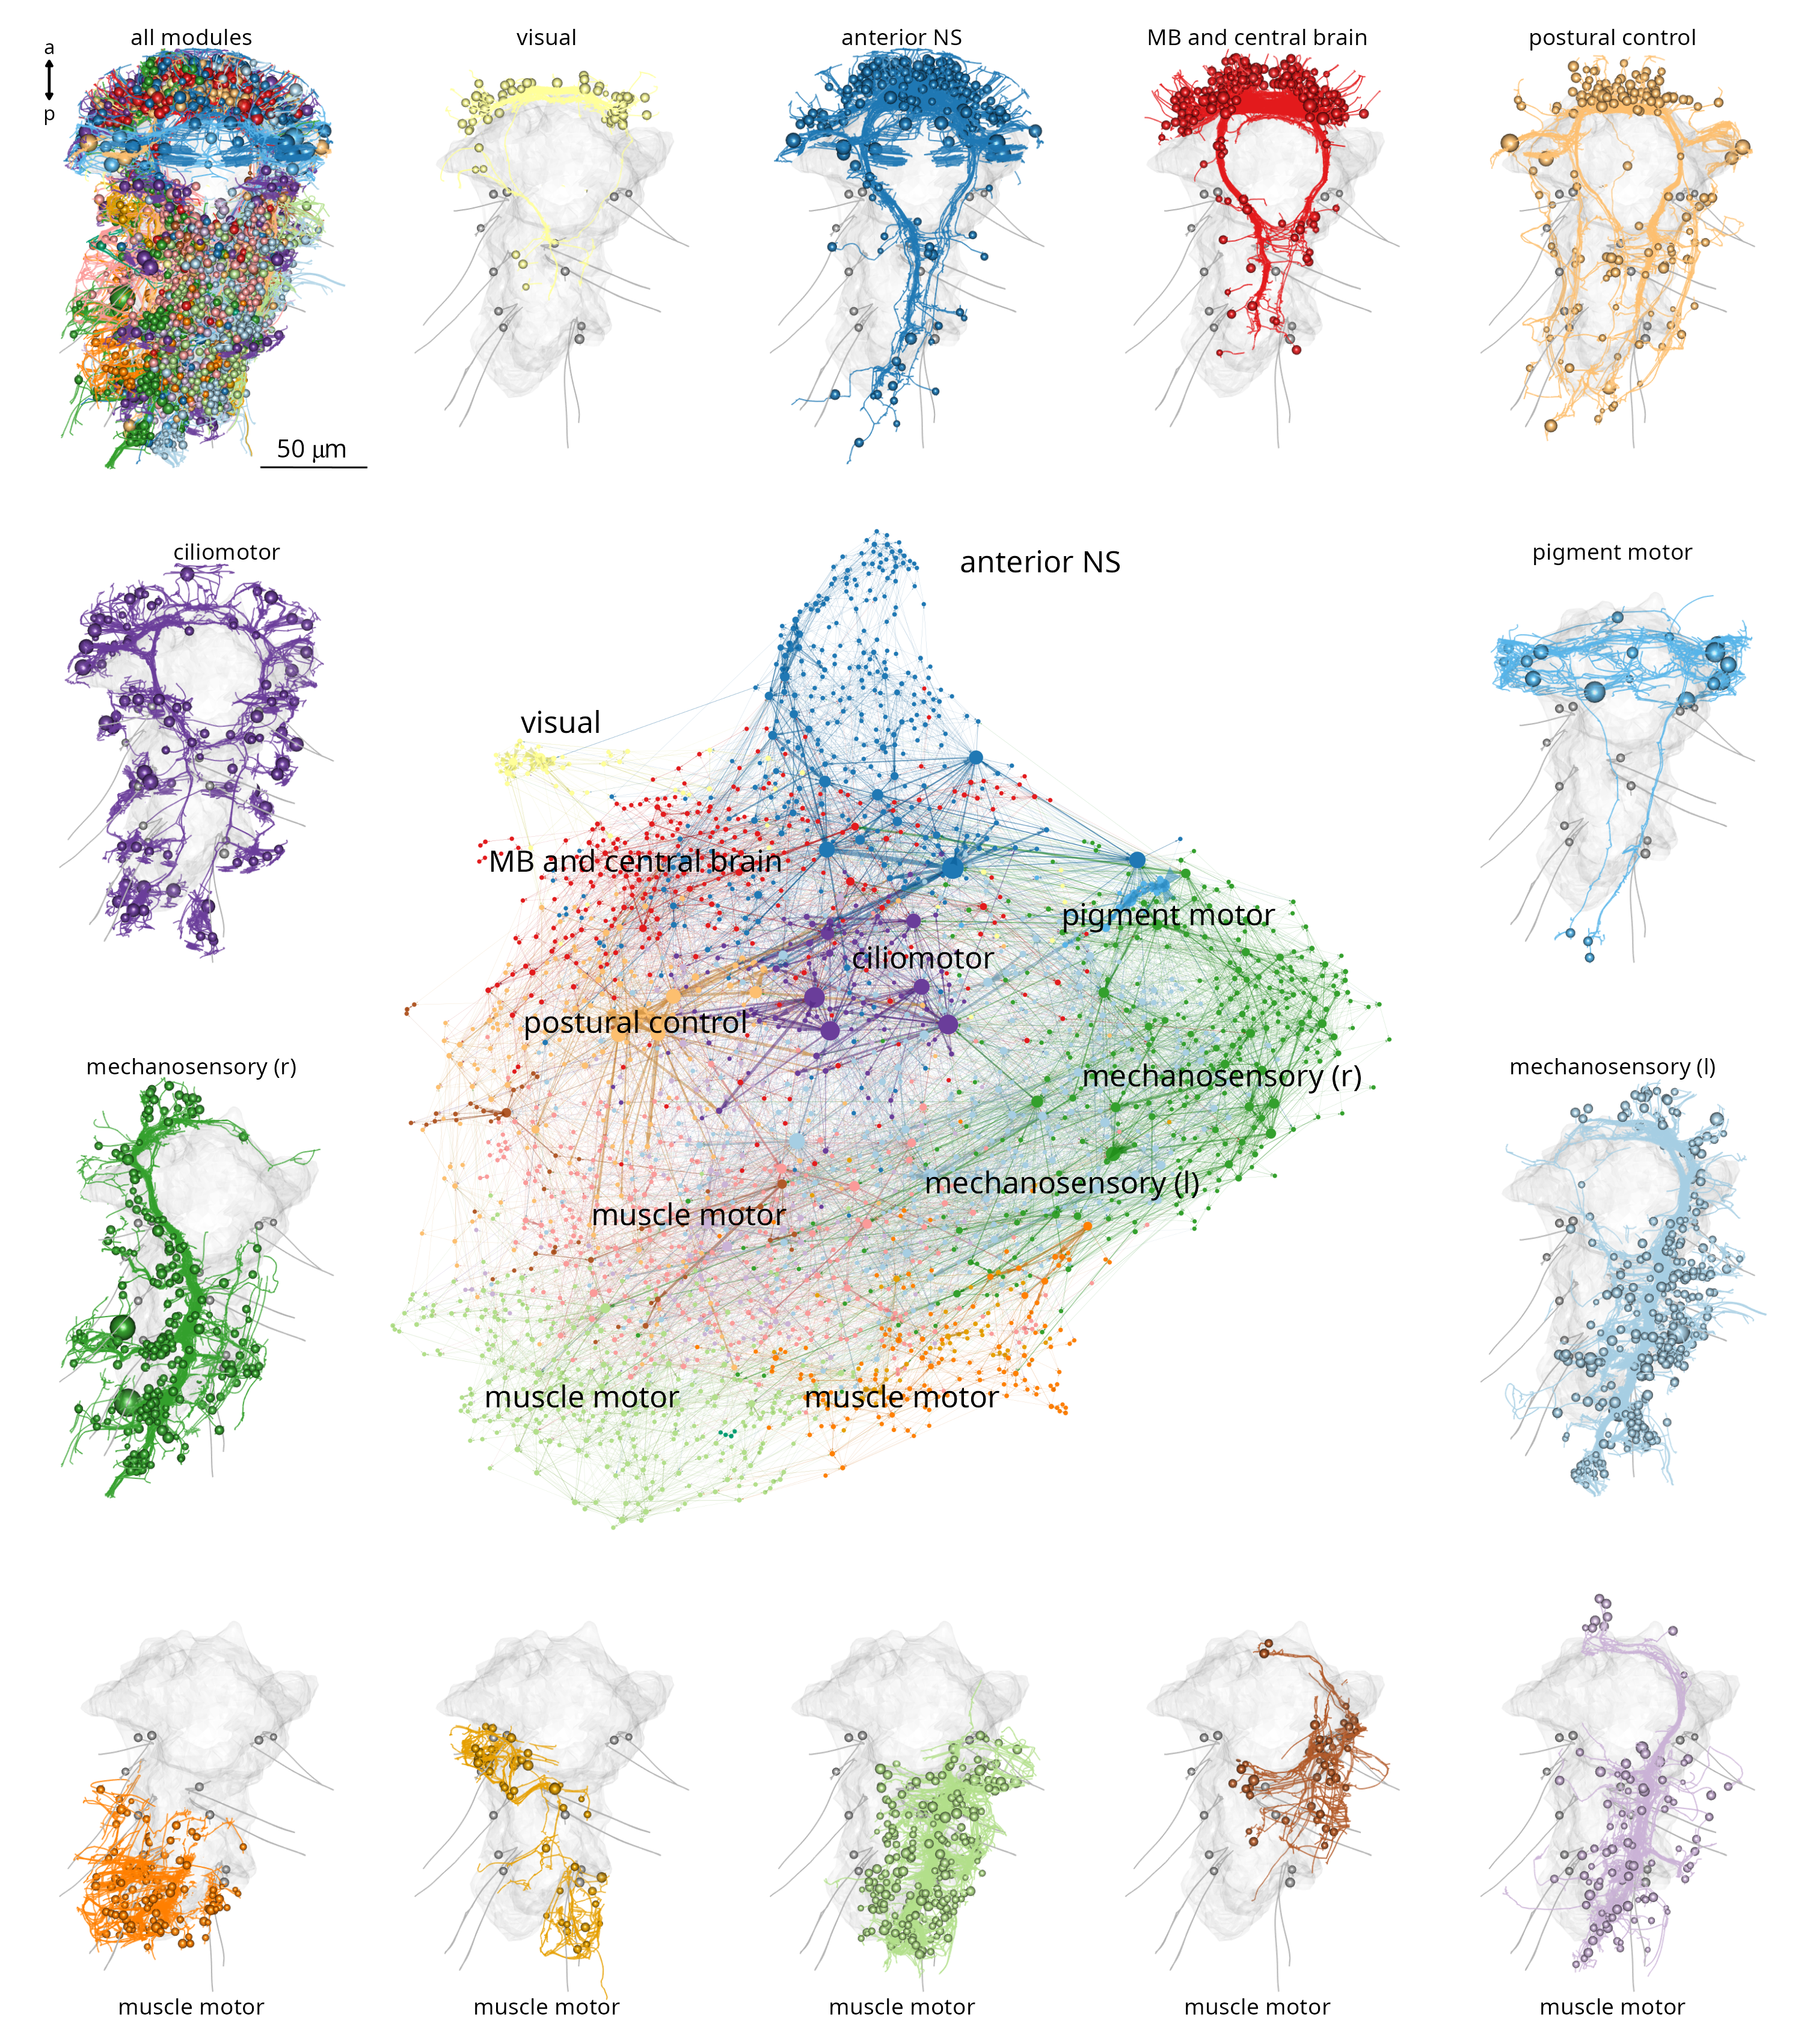
\includegraphics[width=1\textwidth,height=\textheight]{Figures/Figure2.png}

}

\caption{\textbf{Figure 2. Modularity of the \emph{Platynereis} larval
connectome.} Full connectome graph of the \emph{P. dumerilii}
three-day-old larva chemical synapse connectome. Nodes represent
individual cells, edges represent synaptic connectivity. Nodes are
coloured by modules. Node sizes are proportional to weighted degree. The
individual panels show the morphology of all cells in each module with
the outline of the yolk and aciculae shown in grey. Figure 2---source
data 1. Source data of the connectome graph in tibble graph (tbl\_graph)
format saved as an R binary object.}

\end{figure}%

\subsubsection{Cell-type classification and neuronal
diversity}\label{cell-type-classification-and-neuronal-diversity}

In the volume, each skeleton was multiply annotated. Neurons and
non-neuronal cells were categorised into classes (sensory, inter- and
motoneurons, muscle, gland etc.) and further subdivided into cell types.

For classifying neurons into cell types, we used a combination of five
morphological and connectivity criteria: i) position of cell somata, ii)
the morphology of neurite projections (e.g.~branching pattern,
decussating, ascending or descending), iii) the ultrastructure of
sensory specialisations (e.g.~number and type of cilia, microvilli ---
for sensory neurons only), iv) neuropeptide content as determined by the
siGOLD immunolabelling method (Shahidi et al., 2015), and v) synaptic
connectivity. Most cell types show left-right symmetry except for a few
asymmetric or midline neurons (e.g.~SN\_YF5cil, pygPBunp).

Based on these criteria, we classified 966 neurons into 202 cell types
(Supplementary Table 1, Video 1, Figure 3). Most neuronal cell types are
represented by only two cells in the entire body (Figure 3D).

We also categorised the remaining 8,196 cells in the larva. Of these,
3128 were classified into 92 non-neuronal cell types (Supplementary
Table 1, Figure 3---figure supplement 1).

\begin{figure}[H]

{\centering \includegraphics[width=1\textwidth,height=\textheight]{Figures/Figure3.png}

}

\caption{\textbf{Figure 3. Cell-type complement of the three-day-old
\emph{Platynereis} larva.} Segmental distribution and number of sensory
neuron types (A), interneuron types (B) and motoneuron types (C).
Histogram of the number of cells per neuronal (D) and non-neuronal (E)
cell types. (F) Segmental distribution and number of non-neuronal cell
types. The number in each box refers to the number of cells of the
indicated cell type in the indicated segment. Figure 3---source data 1.
Source data for panels A-C. Figure 3---source data 2. Source data for
panel F.}

\end{figure}%

These included epidermal cells (1334 cells), various pigment cells (158
cells of 7 types), muscle cells (853 cells of 53 types, described in
(Jasek et al., 2022)), locomotor ciliated cells (80 cells of 6 types,
described in (Verasztó et al., 2017)), glial cells (78 cells of 3
types), gland cells (54 cells of 6 types), various support and sheet
cells, nephridia, putative migratory cells, parapodial cells producing
chitin chaetae (106 cells) or aciculae (12 cells), and the follicle
cells (566 cells of 5 types) ensheathing them (Supplementary Table 1;
Video 1; Figure 3---figure supplement 1).

In addition, we defined 18 broader neuronal cell groups, containing
neurons of similar morphology (e.g.~head decussating neurons) but in
either differentiated or immature state (e.g.~immature palp sensory
neurons).

The annotations are hierarchical and cell groups can contain one or more
differentiated cell types (Supplementary Table 1). The remaining 5,068
cells are either dividing cells (68 cells), undifferentiated cells that
putatively belong to the neuronal lineage (1597 cells) and various
developing neurons with projections but no or only very few synapses
(2457). These cells were not classified into cell types.

The developing antennae contain 115 cells of which the majority have
only few or no synapses and immature sensory dendrites. In the
developing palps, we found 82 developing sensory neurons. The developing
mouth or stomodeum (675 cells) is lined with 52 immature sensory
neurons.

All cells were annotated in CATMAID (Saalfeld et al., 2009;
Schneider-Mizell et al., 2016) with information representing the above
categories. We also annotated all cells based on their soma position in
the body (e.g.~left or right side, segment 0-3, germ layer etc.)(Figure
3---figure supplement 2). These annotations were used to query the data
and visualise subsets of cells.

Supplementary Table 1 lists all neuronal and non-neuronal cell types,
their main annotations, including morphological, cell-class, segment,
ganglion or sensory organ, neurotransmitter and neuropeptide phenotype,
and main synaptic partners. We also listed all literature references for
previously published neuronal and non-neuronal cells and indicated which
cells are reported here for the first time (105 cell types out of 294).

Querying by two or more annotations allows tallying the number of cells
in different category (e.g.~number of sensory cells with a single
penetrating cilium or the number of gland cells in a particular
segment)(Figure 3---figure supplement 3).

Left-right cell-type pairs have similar arbor morphologies (Figure
3---figure supplement 4). The similar branching patterns for left and
right cells of the same type is also indicated by their similar average
Sholl diagrams (Figure 3---figure supplement 5). Left-right pairs also
have projections at symmetrical positions in the VNC indicating neuropil
stereotypy (Figure 3---figure supplement 6).

Outgoing and incoming synapses in a neuron can be intermingled or
spatially segregated. Interneurons can have mixed or spatially
segregated input-output compartments. Most motoneurons have spatially
segregated input-output compartments (Figure 1L-Q and Figure 3---figure
supplement 7, 8).

\subsubsection{Grouped cell-type-level
connectome}\label{grouped-cell-type-level-connectome}

The cell-type classification allowed us to analyse a grouped synaptic
connectivity graph where cells of the same type were collapsed into one
node and synapse counts were summed (Figure 4A).

This cell-type connectome included 84 sensory, 82 interneurons, 34
motoneuron types and 58 effector cell types (including ciliary band,
muscle, gland and pigmented cell types)(Figure 4---figure supplement 1).

The cell-type graph had 2,410 edges formed by 14,640 synapses (Figure
4).

The correlation of the left and right synapse matrices was 0.91,
indicating a high level of stereotypy of connectivity (Figure 4---figure
supplement 2, Figure 4---figure supplement 3).

The cell-type graph is characterised by network parameters similar to
the \emph{C. elegans} and \emph{C. intestinalis} connectome graphs
(Figure 4---figure supplement 4), suggesting a similar overall circuit
organisation at the level of cell types, but with an order of magnitude
more cells in \emph{Platynereis}.

\begin{figure}[H]

{\centering 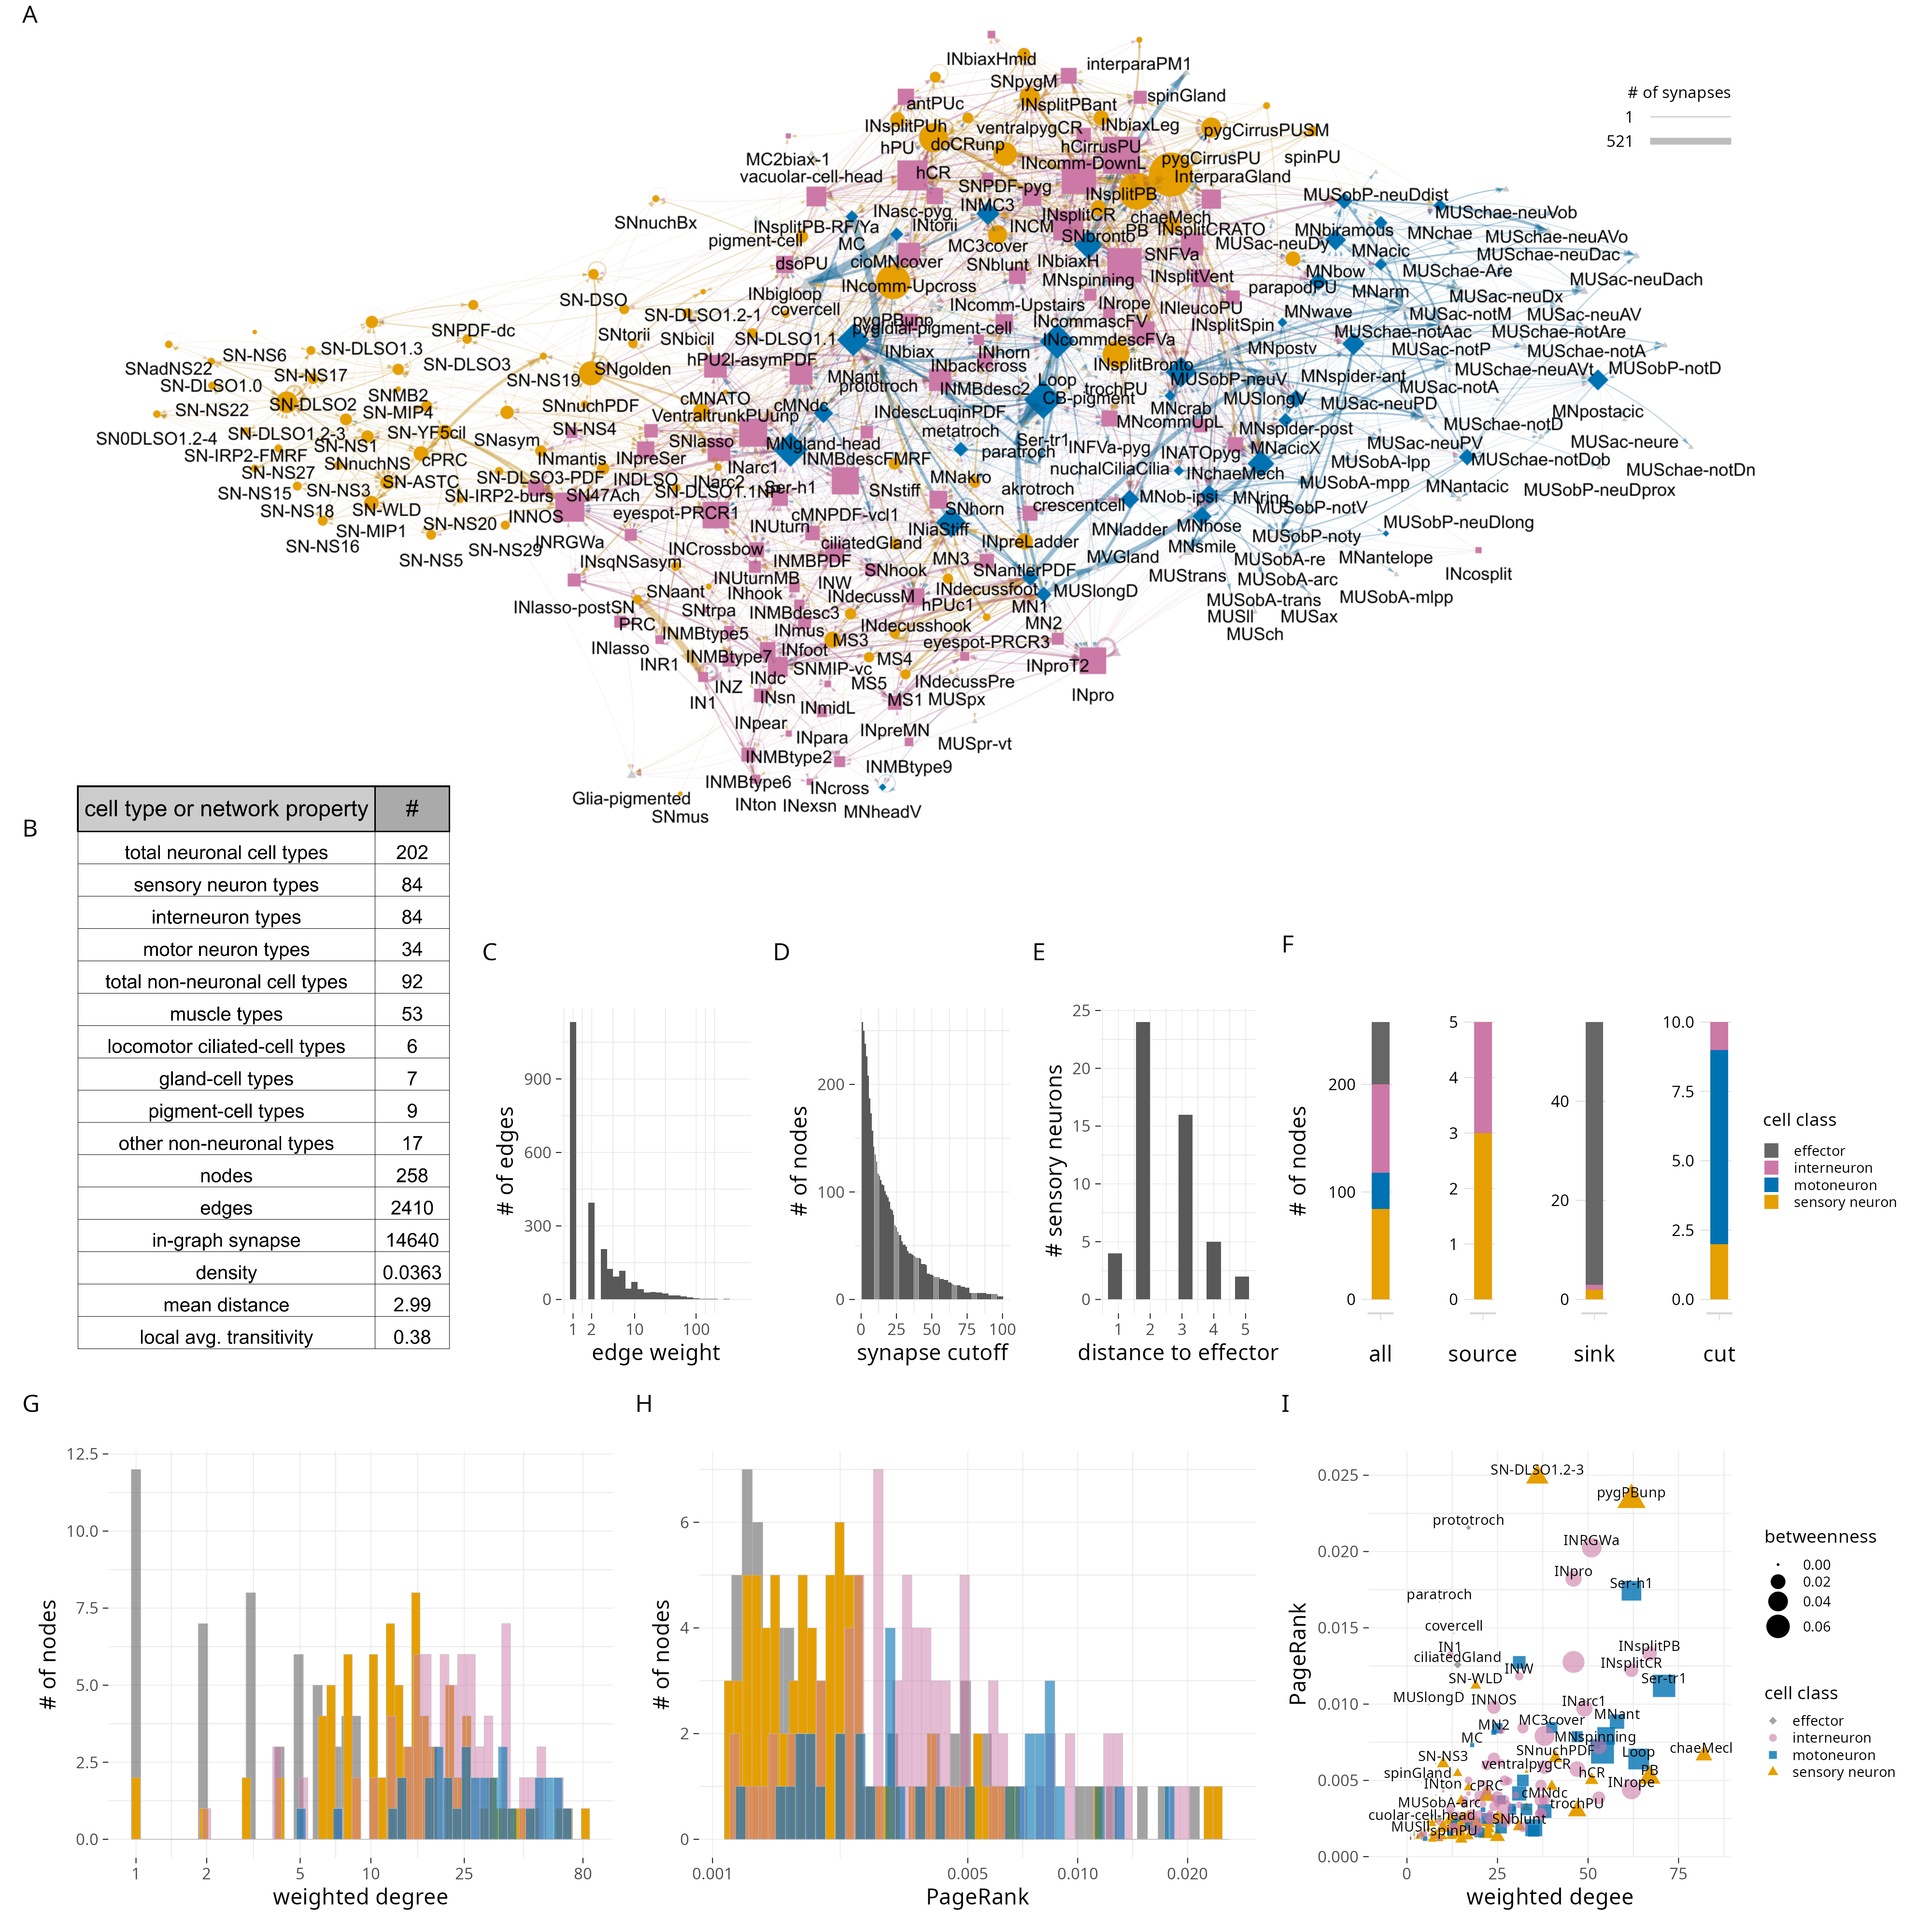
\includegraphics[width=1\textwidth,height=\textheight]{Figures/Figure4.png}

}

\caption{\textbf{Figure 4. Cell-type-level connectivity of the
\emph{Platynereis} larval connectome.} (A) The cell-type connectome of
the three-day-old larva. Nodes represent grouped cells of the same type,
edges represent synaptic connectivity (square root of the sum of
synapses). Nodes are coloured by cell class (SN - orange; IN - magenta;
MN - blue; effector - grey). (B) Table of cell type and network
statistics. (C) Histogram of edge weights. (D) Size of the largest
network after removing edges of increasing weights. (E) Number of
sensory neurons with different path distances from effector cells. (F)
Number of SN, IN, MN and effector cell types in the cell-type-level
connectome shown for all nodes, source nodes, sink nodes and cut nodes.
(G) Histogram of weighted degree of nodes, plotted for each cell class.
(H) Histogram of pagerank of nodes, plotted for each cell class. (I)
Weighted degree of nodes in the cell-type connectome in relation to node
pagerank-centrality. Figure 4---source data 1. Source data of the cell
type connectivity graph in tbl\_graph format saved as an R binary file.}

\end{figure}%

To explore sensory-motor pathways in the grouped graph, we searched for
the shortest directed paths from all sensory neurons to all effector
cells. We identified four sensory neurons with direct motor output
(sensory-motor neurons: eyespot-PRCR3, pygPBunp, pygCirrusPUSM,
hPU2l-asymPDF) and 25 premotor sensory neurons. The maximum number of
hops from sensory neurons to an effector is five. 33 sensory neurons
have no synaptic paths to effectors. 19 of these are neurosecretory
cells with few or no synaptic partners (Williams et al., 2017) (Figure
4---figure supplement 5). For a graph-based visualisation of information
flow, we arranged the nodes according to their relative ratio of
incoming and outgoing synapses (Figure 4---figure supplement 6). This
layout indicates that sensory-evoked activity propagates from sensory
neurons through interneurons and motoneurons to effectors.

\subsubsection{Neurotransmitter and neuropeptides
phenotypes}\label{neurotransmitter-and-neuropeptides-phenotypes}

We could assign neurotransmitters or neuropeptides to 53 (26\%) neuronal
cell types (Figure 5). This was possible either by direct immunogold
labelling for neuropeptides (Shahidi et al., 2015) or by matching the
position and morphology of cells to whole-body gene expression data or
neuronal transgenic reporter expression (Randel et al., 2014; Verasztó
et al., 2017; Vergara et al., 2017).

We annotated 11 cholinergic, 3 serotonergic, 1 dopaminergic, 1
adrenergic, and 4 glutamatergic neuronal cell types. In addition, we
assigned one of 12 neuropeptides to 38 cell types (pigment dispersing
factor --- 12, allatotropin/orexin --- 5, leucokinin --- 1,
proenkephalin --- 1, FVamide --- 5, FMRFamide --- 3, myoinhibitory
peptide --- 3, achatin --- 1, RGWamide --- 1, MLD/pedal peptide --- 1,
IRP2 --- 1, WLD --- 1). Neuropeptides occur in sensory, motor and
interneurons.

In agreement with the large number of neuropeptides expressed in the
larva (Conzelmann et al., 2011; Shahidi et al., 2015; Williams et al.,
2017), 516 connectome neurons contained dense core vesicles, indicative
of peptidergic transmission (Figure 5---figure supplement 1).

We highlight cellular and sensory-effector circuit examples for PDF,
leucokinin and allatotropin/orexin neuropeptides (Figure 5---figure
supplement 2). For example, two leucokinin-expressing interneurons
(INleucoPU) in the first trunk segment are postsynaptic to
mechanosensory PU cells and INsplitPB neurons and synapse on MNladder,
MNcommUpL, and MNwave motoneurons.

These neuropeptide-expressing cells and their mini-circuits pinpoint
potential sites of peptidergic modulation mapped to single-cell
resolution within the whole-body connectome.

\begin{figure}[H]

{\centering 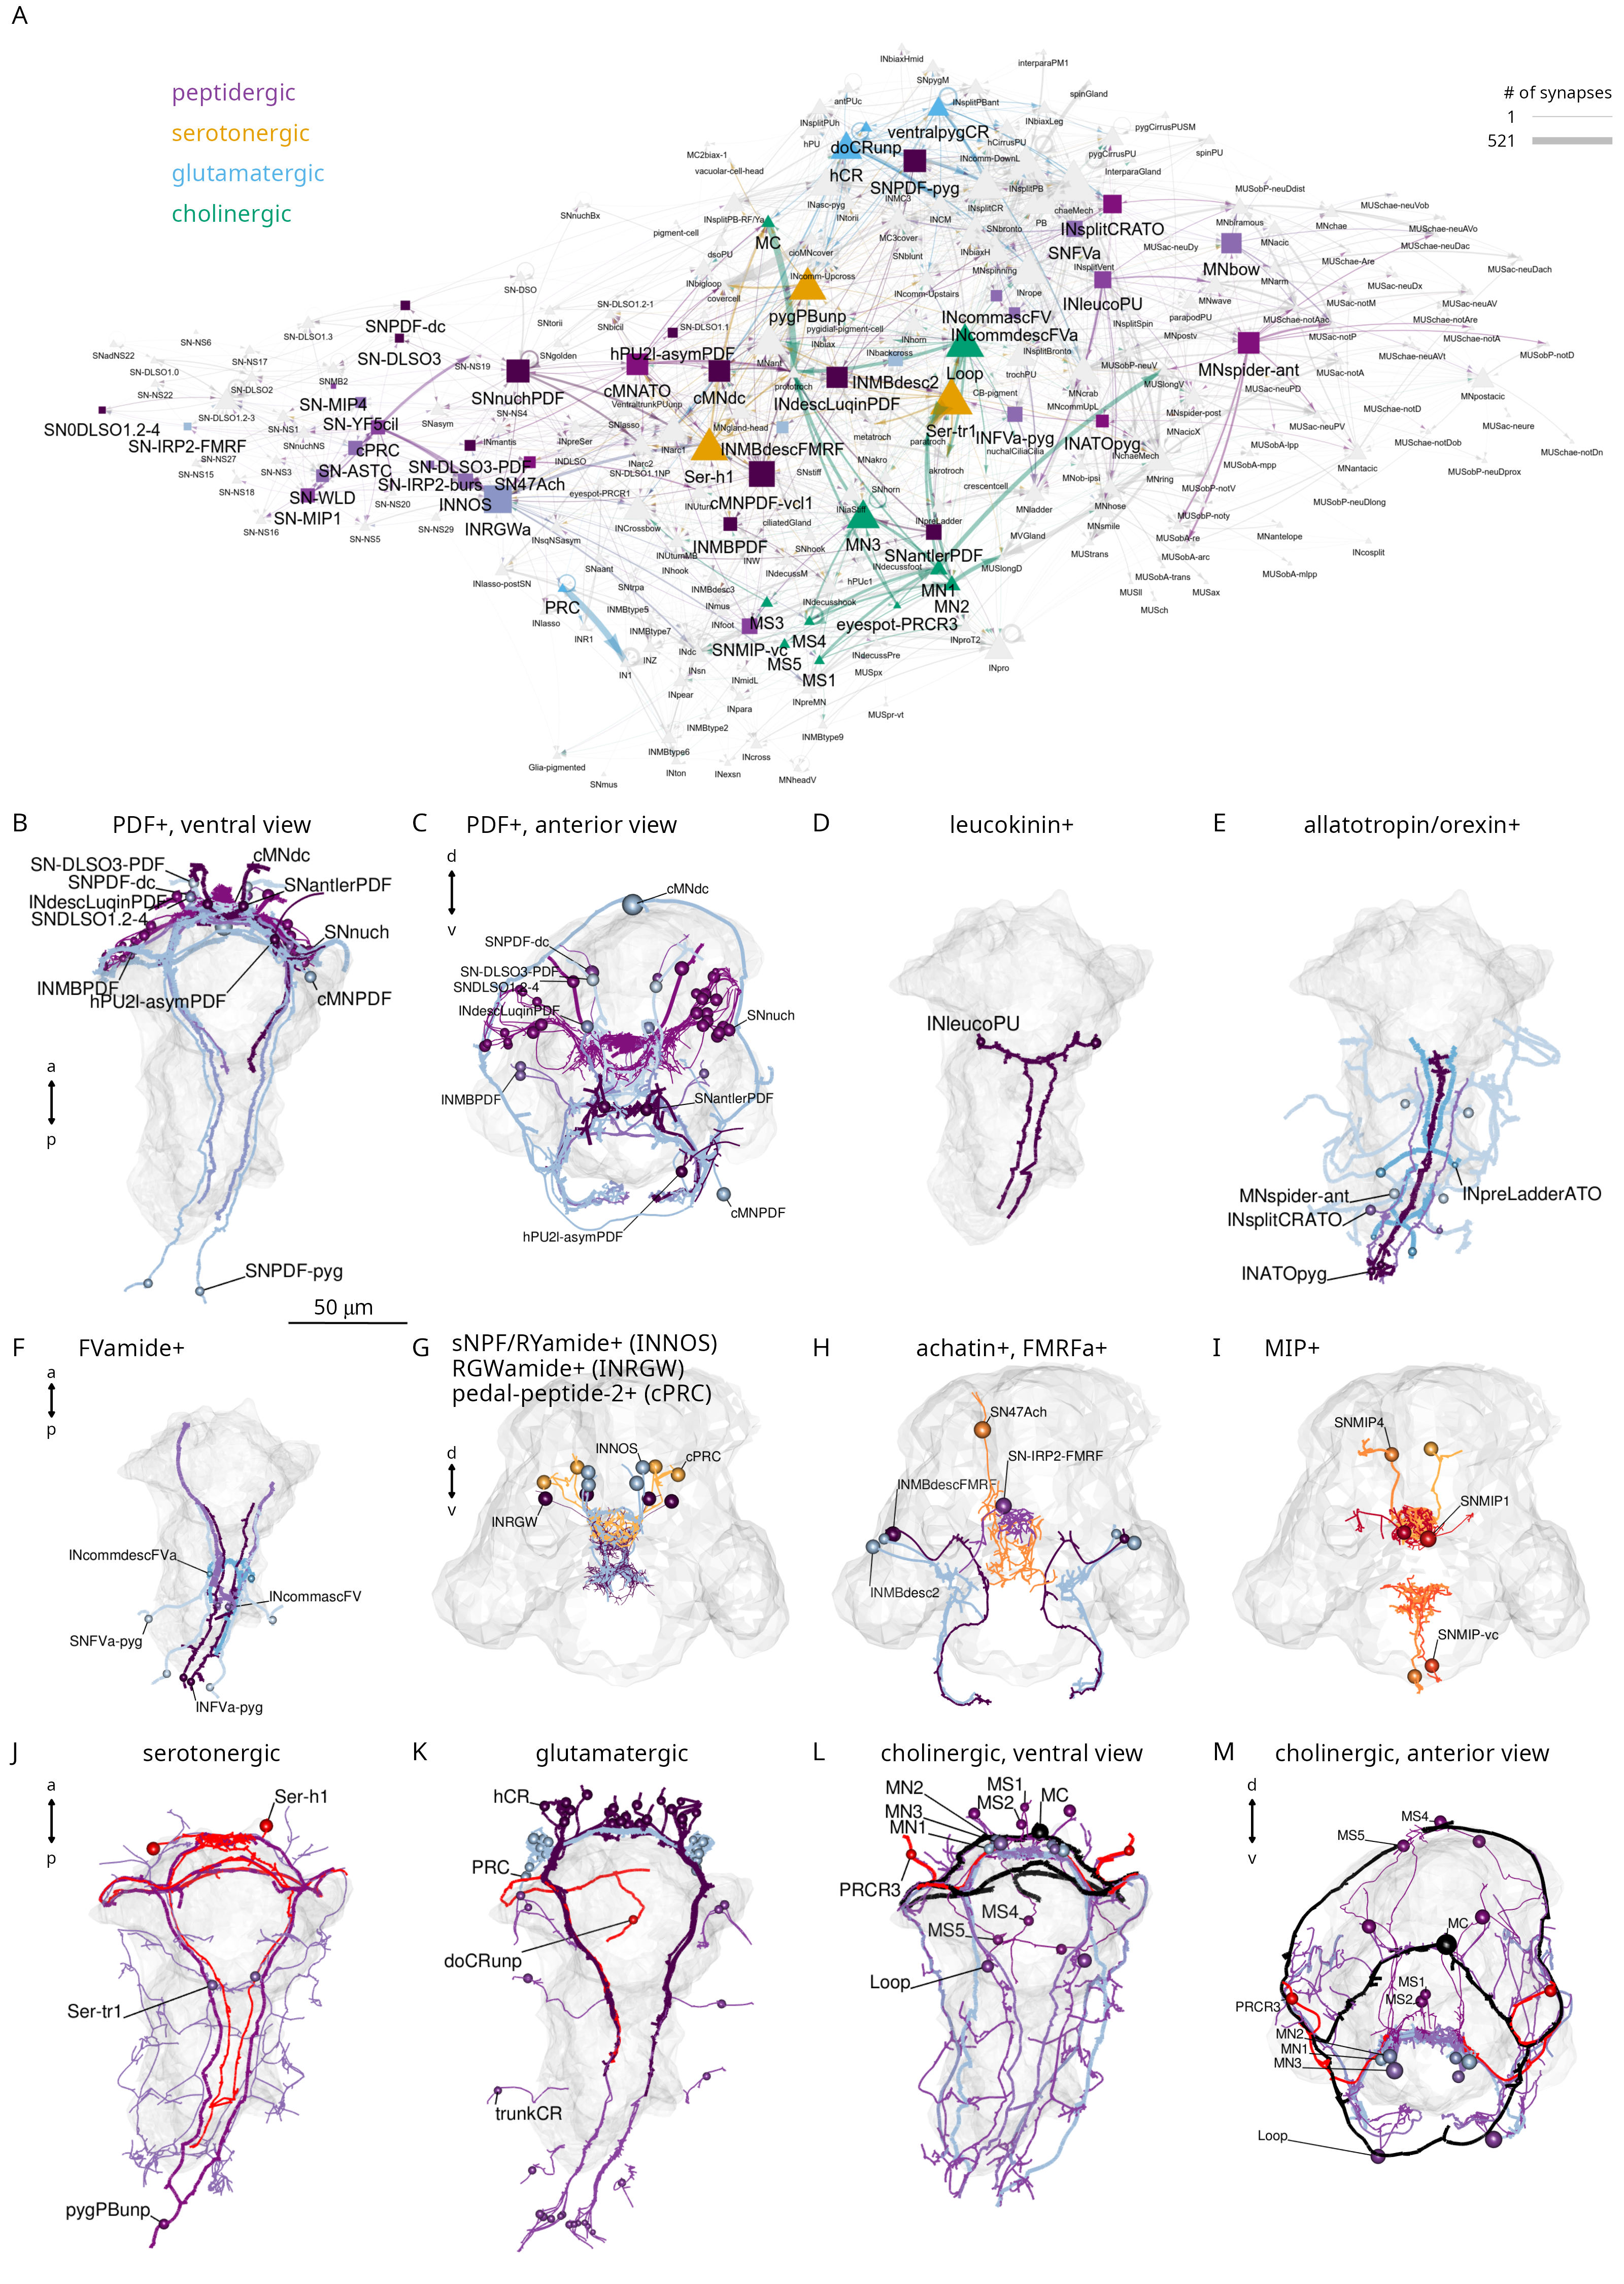
\includegraphics[width=0.7\textwidth,height=\textheight]{Figures/Figure5.png}

}

\caption{\textbf{Figure 5. Transmitter phenotypes mapped at
single-cell-resolution. } (A) The cell-type connectome graph with nodes
coloured based on neurotransmitter phenotype. (B, C) Morphological
rendering of neurons with immunogold labelling for pigment dispersing
factor (PDF) neuropeptide, ventral (B) and anterior (C) views. (D)
Neurons with immunogold labelling for leucokinin. (E) Neurons with
immunogold labelling for allatotropin/orexin. (F) Neurons with
immunogold labelling for FVamide. (G) Neurons with immunohistochemically
mapped expression of sNPF/RYamide, RGWamide and pedal peptide 2/MLD
neuropeptides. (H) Neurons with immunohistochemically mapped expression
of achatin and immunogold- or immunohistochemically-mapped
(SN-IRP2-FMRF) FMRFamide neuropeptide. (I) Neurons with immunogold
(SNMIP-vc) or immunohistochemically mapped expression of myoinhibitory
peptide (MIP) expression. (J) Neurons with immunohistochemically mapped
expression of serotonin and genetically mapped expression of tryptophan
hydroxylase (TrpH), a serotonergic marker. (K) Neurons with genetically
mapped expression of vesicular glutamate transporter (VGluT), a
glutamatergic marker. (L, M) Neurons with genetically mapped expression
of vesicular acetylcholine transporter (VAChT) and choline
acetyltransferase (ChAT), cholinergic markers, ventral (L) and anterior
(M) views.}

\end{figure}%

\subsubsection{Brain ganglia, neuropils, cell types and
circuits}\label{brain-ganglia-neuropils-cell-types-and-circuits}

The annelid nervous system has a ganglionic architecture. In the head of
the \emph{Platynereis} larva, the different head sensory neurons form
several ganglionic clusters, including a median-dorsal sensory cluster,
an apical organ, a dorso-lateral sensory cluster, the adult eyes and
nuchal organs, the antennae, the palps, and the ventro-lateral mushroom
bodies (Video 2; Figure 6A). These distinct sensory cell clusters
project to distinct neuropils in the centre of the brain (Figure 6A-C).
A few sensory cell types are more scattered in the ventro-median head
(Figure 6F). The interneuron somata form clusters in the mushroom
bodies, in the eye and dorso-lateral clusters, the apical organ, and in
the ventro-median domain of the brain (Figure 6D). The interneuron
projections are also organised into overlapping neuropils (Figure 6E;
Video 2).

The head contains 45 sensory neuron types with postsynaptic partners,
including 52 head interneuron types directly postsynaptic to sensory
neurons (Figure 3).

The cell-type annotation and connectivity information for all
differentiated neurons allowed us to investigate the cellular
composition and circuitry of the different head ganglia and cell types.

\begin{figure}[H]

{\centering 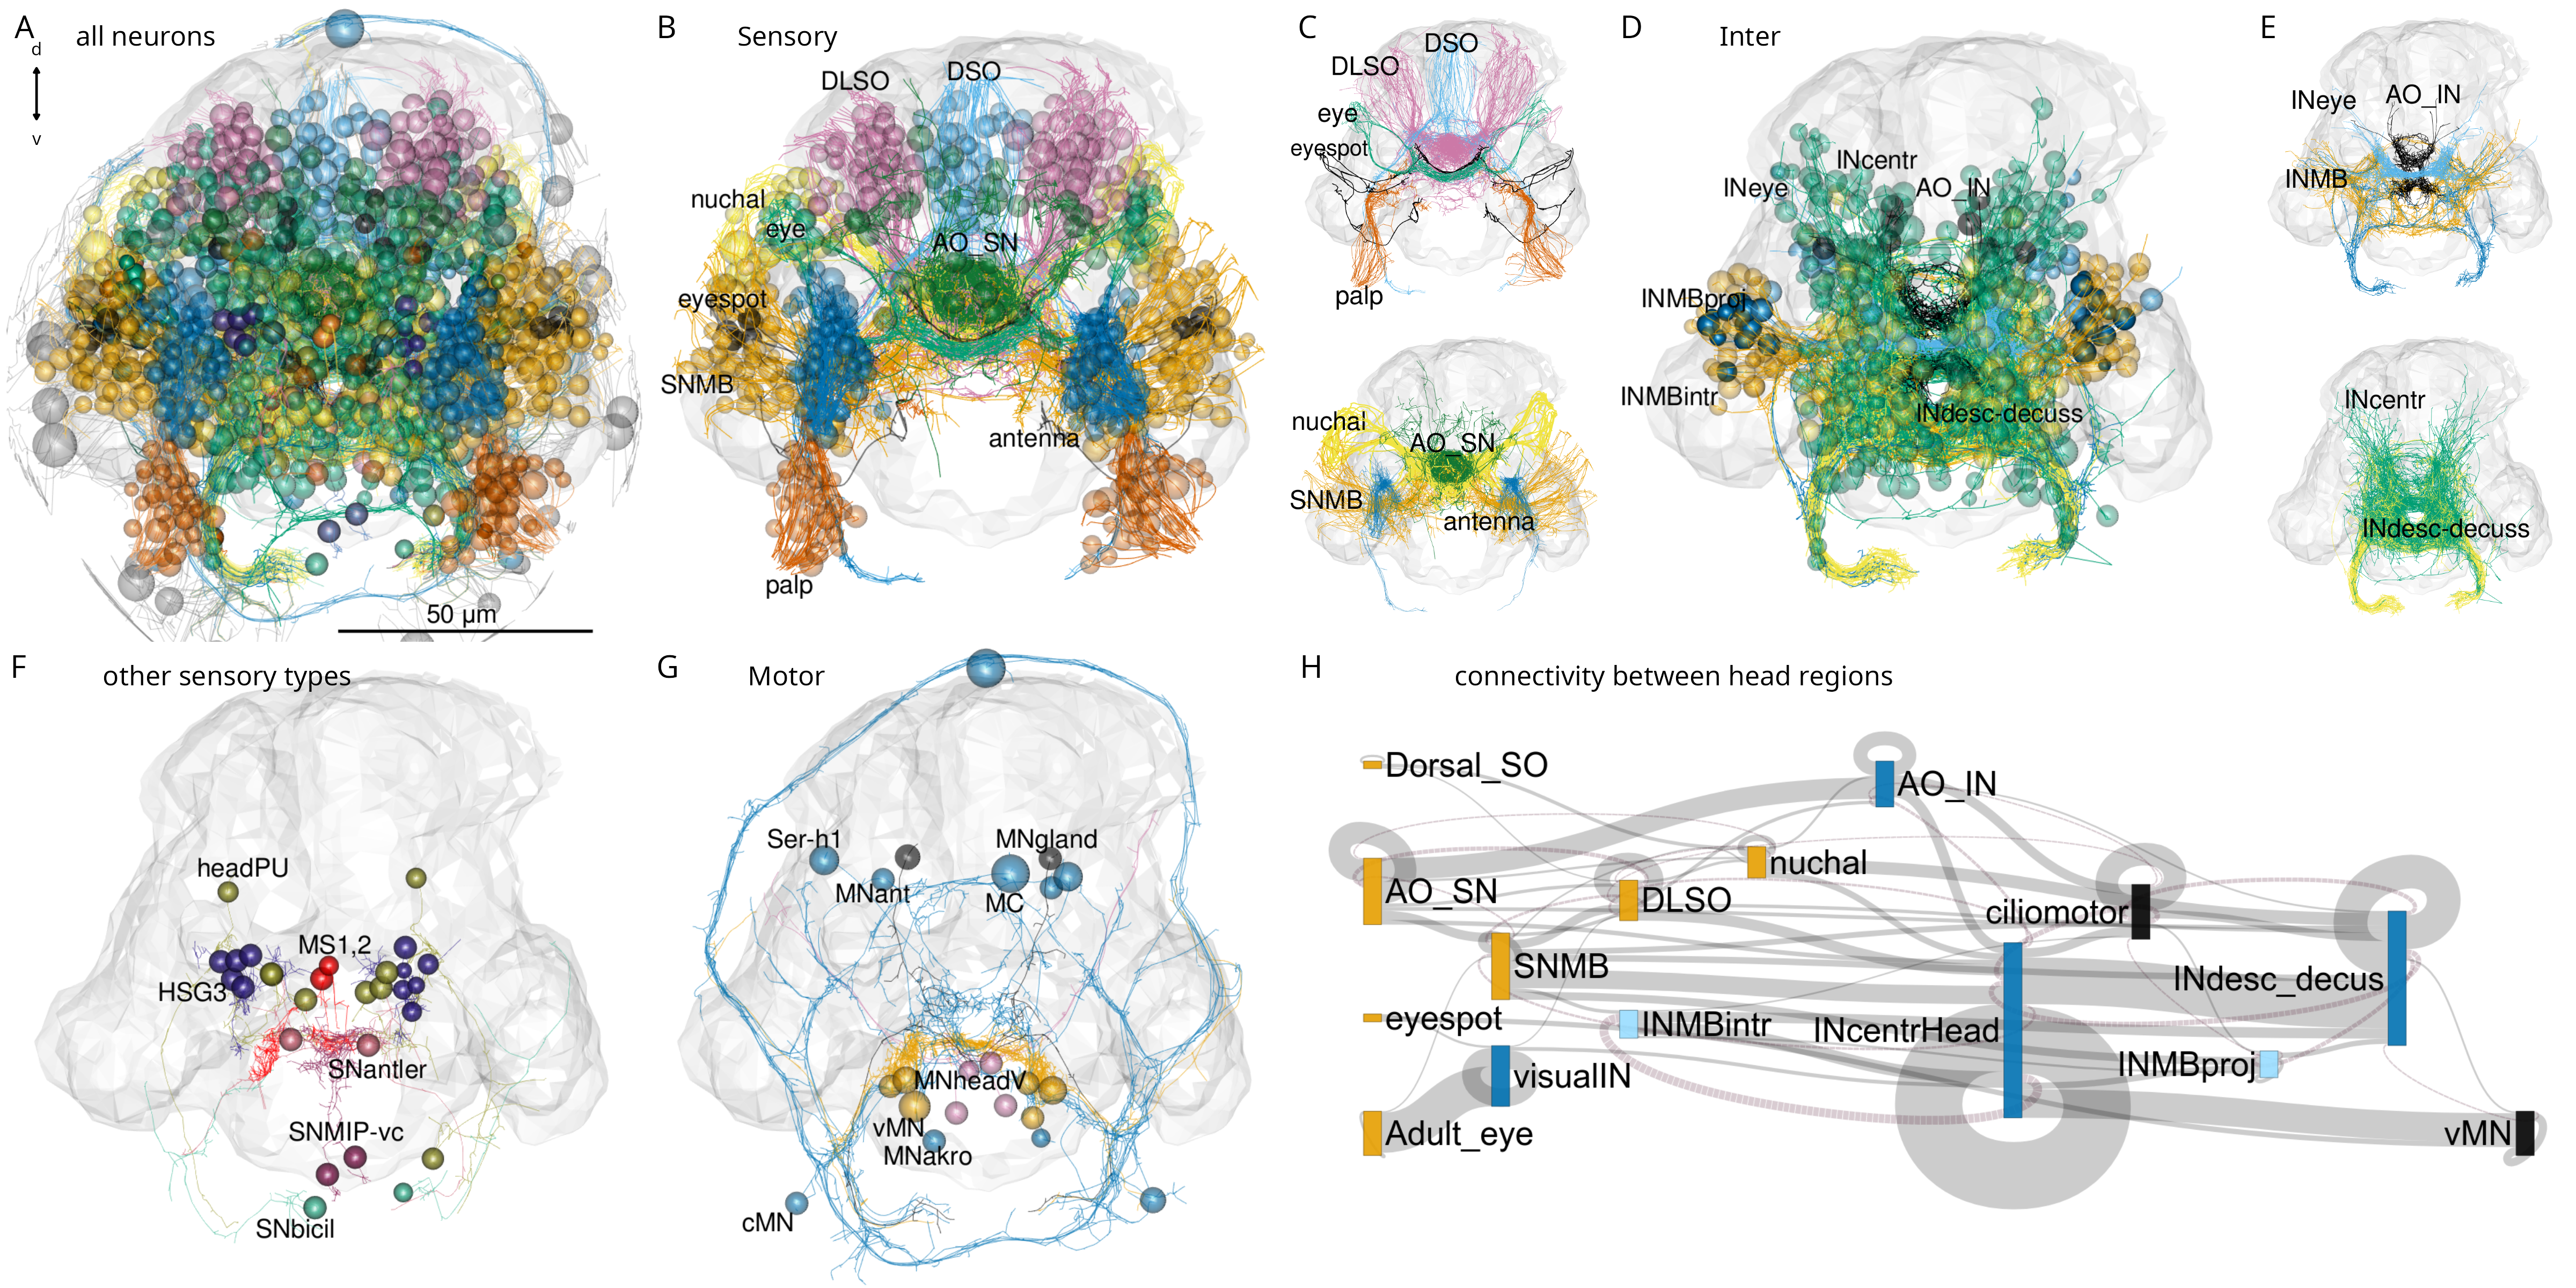
\includegraphics[width=1\textwidth,height=\textheight]{Figures/Figure6.png}

}

\caption{\textbf{Figure 6. Anatomy of head neuropils and global
organisation of brain connectivity} (A) Morphological rendering of all
head neurons. (B) Head sensory neurons coloured by head sensory ganglia.
Abbreviations: DLSO, dorso-lateral sense organ; DSO, dorsal sense organ;
SNMB, mushroom body sensory neuron; INMB, mushroom body interneuron;
INMBintr, mushroom-body-intrinsic interneuron; AO SN, apical organ
sensory neuron; AO IN, apical organ interneuron; INcentr, central brain
interneuron; vMN, ventral motoneuron. (C) Same cells as in (B) rendered
without the cell soma to show neuropil organisation. (D) Head
interneurons coloured by head ganglia. (E) Same cells as in (D) rendered
without the cell soma to show neuropil organisation. (F) Rendering of
other sensory cell types that do not form separate neuropils. (G)
Rendering of head motoneurons. (H) Sankey circuit diagram showing
information flow (from left to right) based on synaptic connectivity
between cell categories of head ganglia. Bars represent groups of
neurons, grey connecting lines represent synaptic connections
(pre-to-post organised left-to-right). Magenta lines represent
right-to-left connections. Only connections with \textgreater10 synapses
are shown. Figure 6---source data 1. Connectivity matrix of the network
in panel H.}

\end{figure}%

Information flows from various sensory neuron clusters to head
interneurons that converge on ciliomotor, head ventral motoneuron
(vMNs), and head descending interneuron groups (Figure 6H). There is
recurrent connectivity between some interneuron clusters (e.g.~between
INMBintr and INcentrHead) and within-cluster connectivity
(e.g.~visualIN, INcentralHead).

One direct motor output of head circuits are three pairs of ventral head
motoneurons (the vMNs: MN1, MN2, MN3)(Randel et al., 2015; Randel et
al., 2014). These decussating (crossing the midline before descending)
motoneurons are at the core of a postural control module (Figure 2;
Figure 7A-D). Their inputs include central head interneurons and several
premotor sensory neurons (SNantler, MS, eyespotPRCR3) that directly
synapse on the vMNs. The vMNs have a decussating morphology and
innervate contralateral ciliated cells and ventral and dorsal
longitudinal muscles, controlling trunk bending and the laterality of
ciliary beating (Randel et al., 2015; Randel et al., 2014).

Another motor output from the head is two types of exocrine glands in
the first segment (ciliatedGland, MVgland). These are innervated by two
MNgland-head gland-motor neurons. The MNgland-head cells receive input
from the rhythmically active serotonergic Ser-h1 ciliomotor neurons
(Verasztó et al., 2017) suggesting a link between ciliary activity and
glandular secretion.

Furthermore, several head ciliomotor neurons directly innervate
locomotor ciliary bands (Verasztó et al., 2017) (MC, Ser-h1, MNant,
vMN). Of these, the MNant cells receive direct input from several head
sensory neurons (SNhook, SNtorii, SNantler, SNhorn)(Figure 7F). The vMN
and MNant motoneurons thus seem to integrate multiple direct sensory and
other inputs.

Sensory integration also characterises the visual system. Here, the
visual eye photoreceptors (PRC) share a postsynaptic interneuron (INR)
with the PRCR1 photoreceptors of the eyespots (Figure 7G-H).

To identify neurons with possible integrative function, we ranked cells
by the number of presynaptic and postsynaptic cell-type-level partners.
We also ranked cells by various node-centrality measures including node
weighted degree, pagerank, betweenness and authority (Figure 7J, K;
Figure 7---figure supplement 2).

The MNant and vMN motoneurons have among the highest number of
presynaptic partners. Among the interneurons, INRGW, INarc1 and INW
integrate the largest number of inputs.

Regarding the multiplicity of outputs, the head collar receptor neurons
(hCR) that mediate a startle response (Bezares-Calderón et al., 2018)
stand out with the largest number of postsynaptic cell types.

Some sensory neurons directly connect to muscle-motor, ciliomotor or
pigment-motor neurons (e.g.~eyespotPRC\_R3, MS cells, SNhook, SNblunt)
(Figure 6---figure supplement1, Figure 7) or to effector cells
(e.g.~eyespotPRC\_R3, hPU2l\_asymPDF)(Figure 7, Figure 4---figure
supplement 5).

Analysis of connectivity (\textgreater2 synapses) only between head
sensory and interneurons revealed a skewed distribution with many
sensory neurons only synapsing on one interneuron type and many
interneurons only receiving input from one sensory neuron type (Figure
7---figure supplement 2A, B).

At the other end of the distribution, the head CR neurons have eight and
SNlasso have five types of postsynaptic interneuron partners, suggesting
that these cells recruit extended downstream circuits (Figure 7---figure
supplement 3A, E).

Some interneurons and motoneurons are directly postsynaptic to several
distinct sensory neuron types (up to 9, \textgreater2 synapses)(Figure
7---figure supplement 3). Among the interneurons, INRGWa, INarc1 and
INcrossbow have \textgreater4 presynaptic sensory neuron partners. The
MNant and ventral head motoneurons (vMN) receive direct input from 2-5
sensory neuron types (Figure 7, Figure 7---figure supplement 2-3).

The interneurons with the highest number of presynaptic interneuron
partners are the INW cells (Figure 7---figure supplement 3D). INWs are
projection neurons of the central brain with decussating axons that
delineate a V-shaped brain neuropil (Figure 9P; Figure 7---figure
supplement 3H). They receive inputs from the mushroom body and central
brain (see below). The interneurons with the largest number of
postsynaptic interneuron partners are the INRGWa cells of the anterior
neurosecretory nervous system (Figure 7---figure supplement 3F, G).

\begin{figure}[H]

{\centering \includegraphics[width=1\textwidth,height=\textheight]{Figures/Figure7.png}

}

\caption{\textbf{Figure 7. Brain circuits and cell types} (A) Schematic
diagram of the postural control system of vMN neurons with their direct
sensory neuron inputs and motor outputs. (B-C) Morphological rendering
of neurons and effector cells of the postural control system, ventral
(B) and anterior (C) views. (D) Sankey diagram of synaptic connectivity
in the postural control system. (E) Sankey diagram of synaptic
connectivity of MNant motoneurons. (F) Morphological rendering of the
MNant ciliomotor circuit, anterior view. (G) Morphological rendering of
eyespot and visual eye photoreceptors and their direct postsynaptic
partners. (H) Sankey diagram of synaptic connectivity of the eyespot and
visual eyes. (I) Histogram of the number of cells per head neuronal cell
type. (J) Number of presynaptic neuron types for different head cell
types (at least 4 synapses). (K) Number of postsynaptic cell types for
different head neuronal cell types (\textgreater3 synapses). In B, C, F,
G the outline of the yolk is shown for reference. Figure 7---source data
1. Connectivity matrix of the network in panel D. Figure 7---source data
2. Connectivity matrix of the network in panel E. Figure 7---source data
3. Connectivity matrix of the network in panel H.}

\end{figure}%

\subsubsection{Mushroom-body anatomy and
circuits}\label{mushroom-body-anatomy-and-circuits}

Nereid annelids have a pair of mushroom bodies with morphological and
molecular similarities to arthropod mushroom bodies (Tomer et al.,
2010). In \emph{Platynereis}, the mushroom bodies start to develop in
the larva. In the six-day-old volume, the partial reconstruction of
neurite projectiones revealed the presence of both sensory and
interneurons in the mushroom bodies. Some of the sensory neurons were
found to project to the anterior neurosecretory neuropil (Arendt et al.,
2021; Vergara et al., 2021). Here we present the complete reconstruction
of the developing mushroom bodies and their circuits in the
three-day-old larva (Video 3; Figure 8).

The mushroom bodies (MBs) are formed by a pair of ventrolateral brain
ganglia. They comprise both sensory and interneurons (SNMB and
INMB)(Figure 8A-D). Most SNMB cells project to two lateral MB neuropils
and a few to the anterior neurosecretory plexus (Figure 8B), in
agreement with the projection reconstructions (Vergara et al., 2021).

We classified INMBs into intrinsic (MBintrIN) and output projection
(MBON) types (Figure 8C-D). MBintrINs project to the MB neuropils, MBONs
project ventrally to the VNC or to the developing mouth
(stomodeum)(Figure 8C-G; Video 3).

\begin{figure}[H]

{\centering 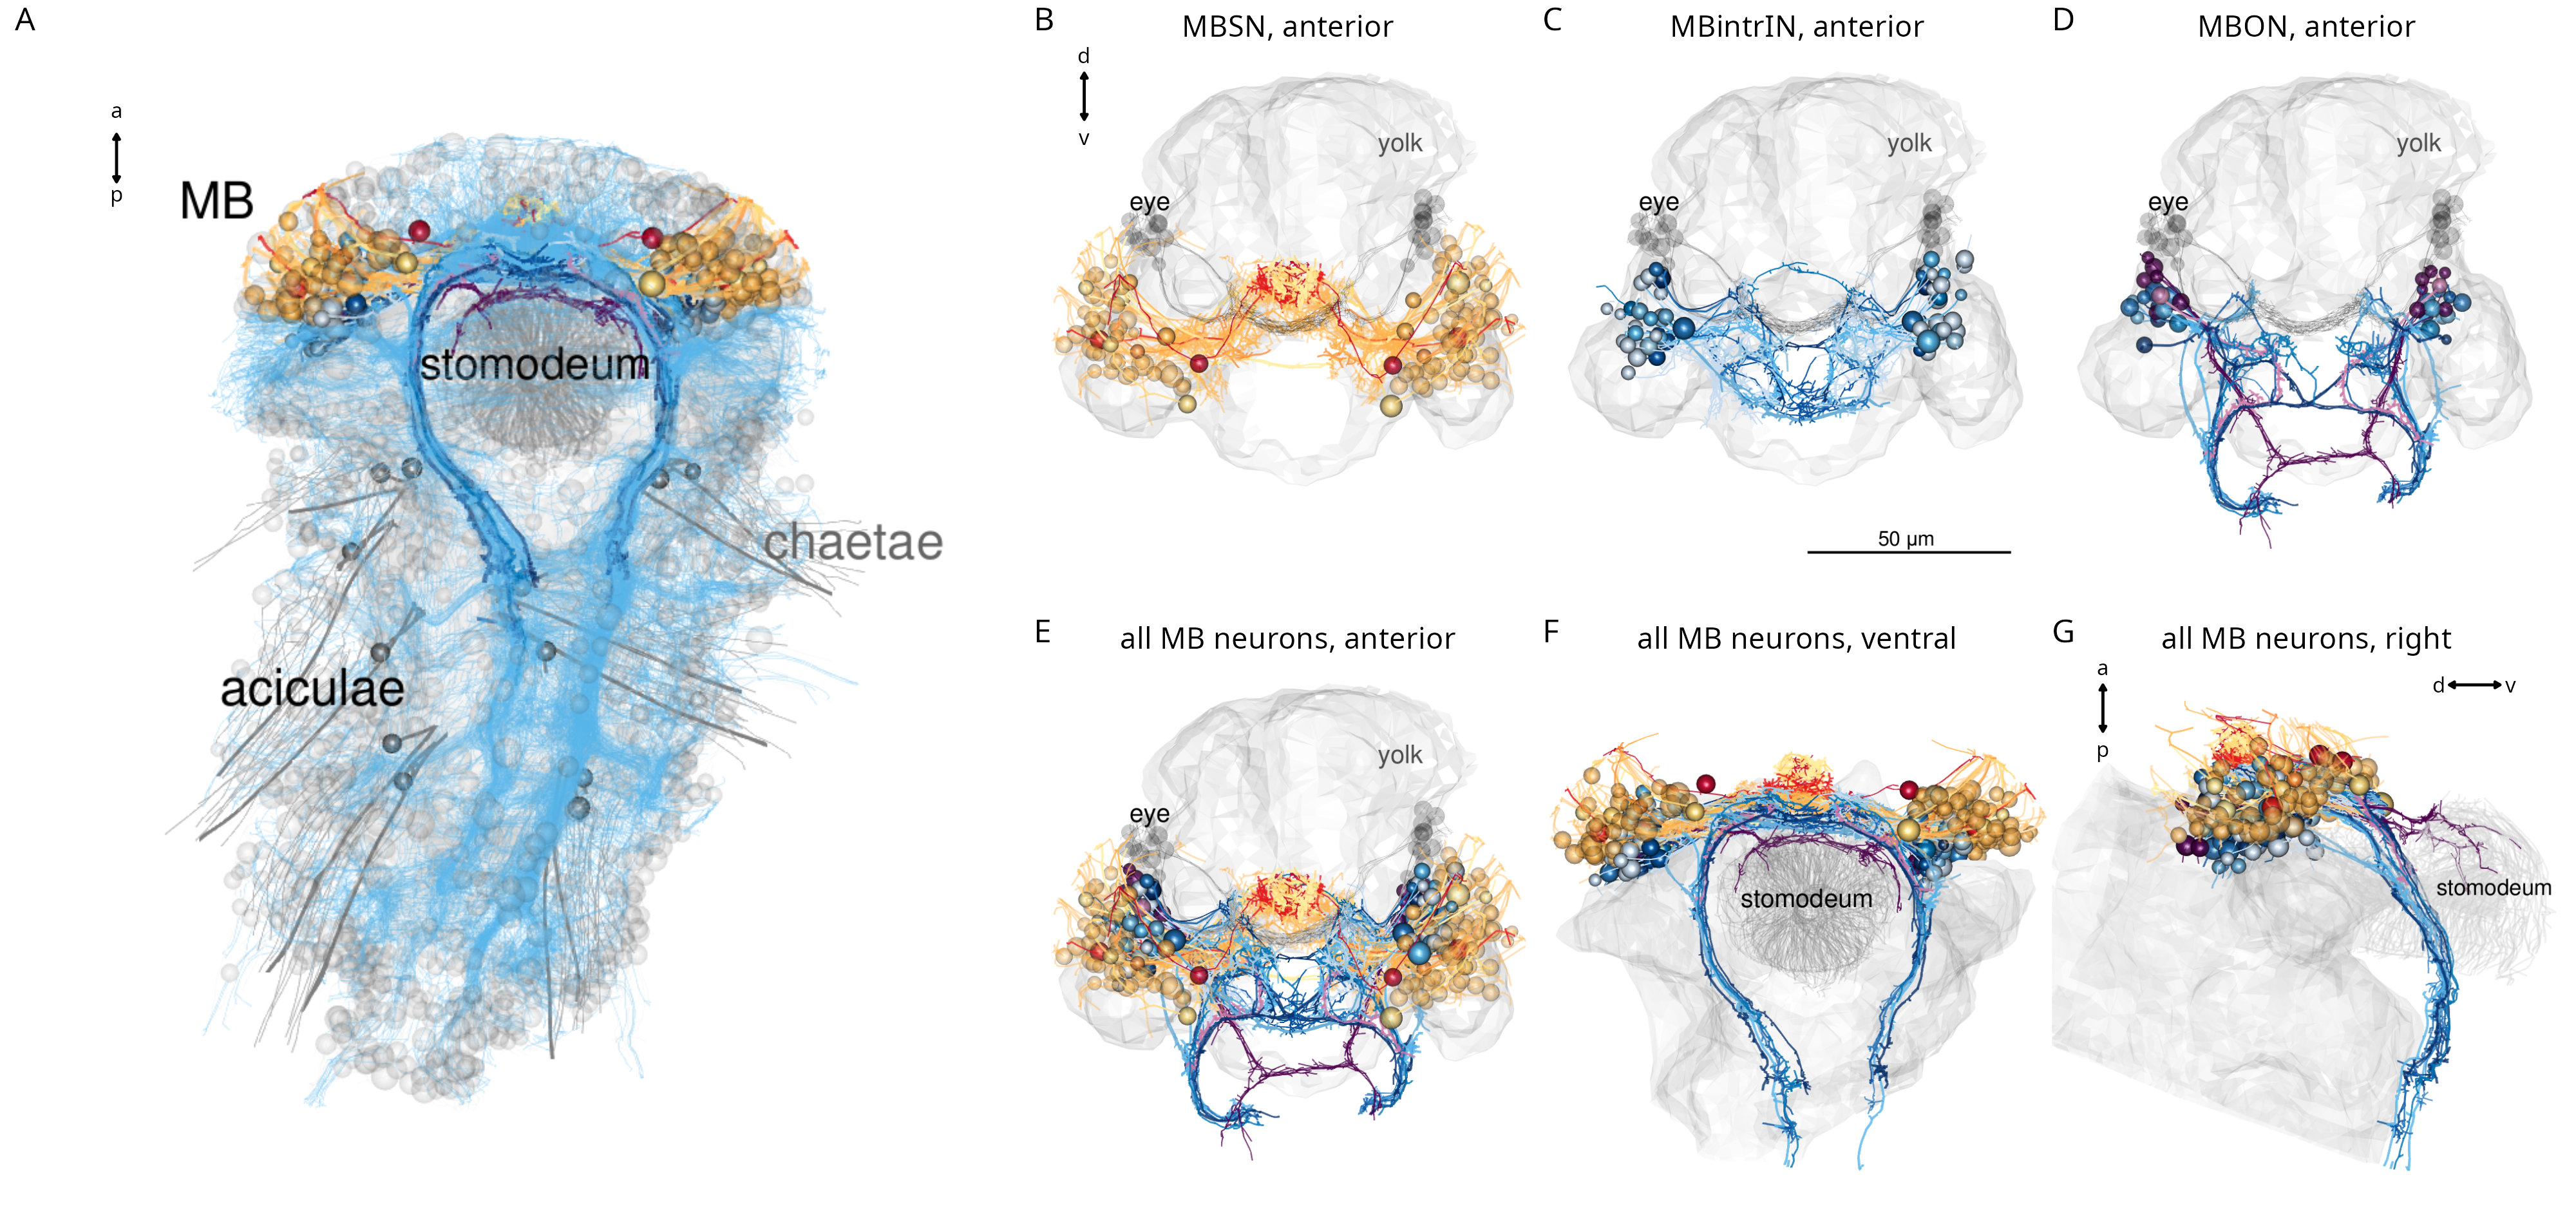
\includegraphics[width=1\textwidth,height=\textheight]{Figures/Figure8.png}

}

\caption{\textbf{Figure 8. Anatomy of the \emph{Platynereis} mushroom
bodies} (A) Morphological rendering of the \emph{Platynereis} mushroom
bodies in the context of the entire nervous system (neurites shown in
cyan), ventral view. (B-G) Morphological renderings of all mushroom body
sensory neurons (B), intrinsic interneurons (C), output neurons (D), and
all neurons in three different views (E-G). The visual eyes, yolk
outline and the stomodeum are shown in grey for reference.}

\end{figure}%

Besides MB-intrinsic sensory neurons, MBs receive sensory input from the
antennae, the palps and two further sensory neuron types (SNbronto,
SNstiff)(Figure9A-D). These sensory inputs are mostly to the MBONs.
SNMBs connect to MBINs, central brain interneurons and the MNant
ciliomotor neurons (Figure 9A). There is cell-type-specific connectivity
between sensory neuron types and interneurons, with groups organised
into specific micro-circuits (Figure 9B, E-G, Figure 9---figure
supplement 1A, B). MBINs connect to distinct central brain interneuron
or projection-neuron types that in turn provide distinct inputs to trunk
circuits (Figure 9H-Q, Figure 9---figure supplement 1C, D), including
motor innervation (Figure 9O).

The morphology and connectivity of distinct mushroom body cell types
shows left-right symmetry. The Sholl diagrams are similar for left-right
pairs and the correlation coefficient of the left and right connectivity
matrices is 0.76 (Figure 9---figure supplement 2).

The outputs of the mushroom body circuits also include projection
neurons of the central brain, including the INW, INlasso, INproT2 and
INdecussHook neurons (Figure 9H-Q). Among these the INproT2 neurons are
premotor neurons synapsing on trunk MNring motoneurons, indicating a
shallow sensory-motor organisation of mushroom-body outputs.

The overall architecture of the \emph{Platynereis} MB is multilayer,
parallel and feed-forward, with only very weak recurrent connections or
lateral connections between the feed-forward networks (Figure 9B; Figure
9---figure supplement 1). The circuit also shows a fan-out fan-in
architecture, with the sensory neurons diverging to several IN targets
(e.g.~SNtorii to INtorii, INbigloop and INhorn) and post-MB interneurons
receiving converging input (e.g.~INW from INhook, INlasso, INMBtype5-6,
and SNlasso). This multilayer perceptron architecture may support the
formation of associative memories, as proposed for memory circuits in
cephalopods (Shomrat et al., 2011).

\begin{figure}[H]

{\centering 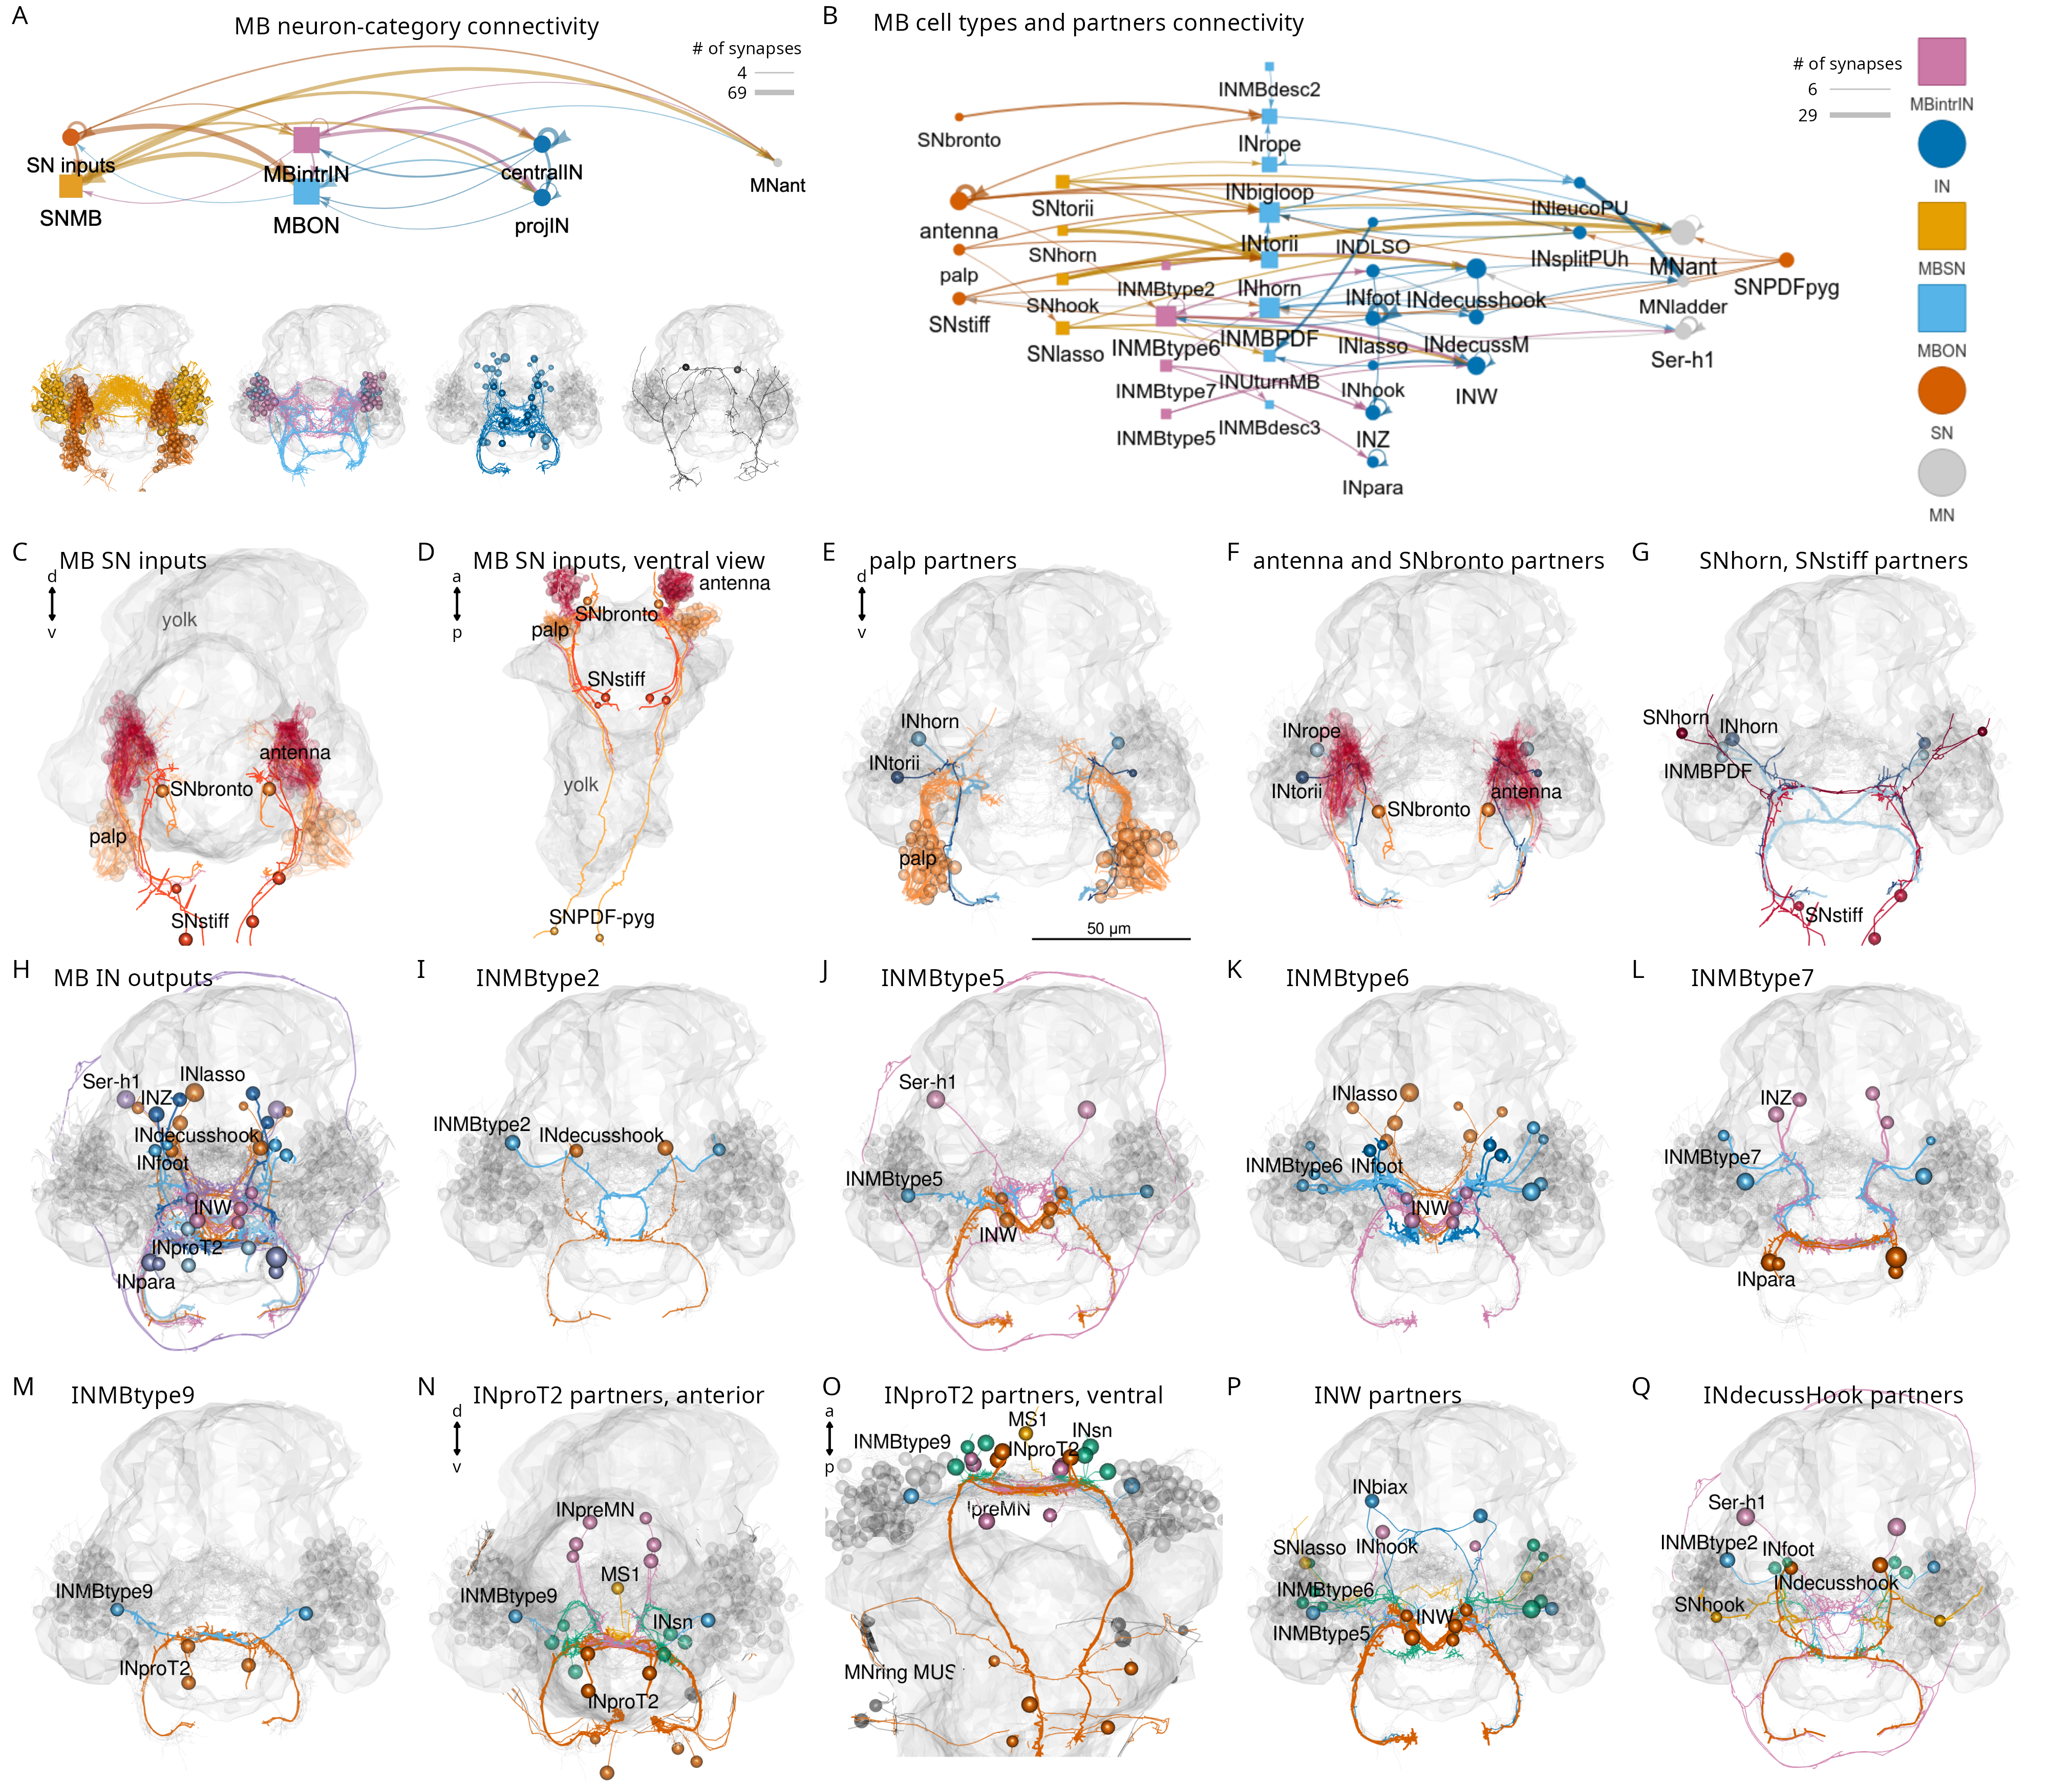
\includegraphics[width=1\textwidth,height=\textheight]{Figures/Figure9.png}

}

\caption{\textbf{Figure 9. Parallel circuit organisation of the mushroom
bodies} (A) Connectivity of the mushroom body by neuron category with
morphological rendering for each category shown below. (B) Connectivity
of mushroom-body neurons and their outputs. Nodes represent neurons
grouped by cell type, arrows show synaptic connectivity. (C-D) Sensory
inputs to the mushroom bodies (other than SNMB), anterior (C) and
ventral (D) views. (E) Palp sensory neurons and their interneuron
targets in the mushroom body. (F) Antennal and SNbronto sensory neurons
and their interneuron targets in the mushroom body. (G) SNhorn and
SNstiff sensory neurons and their interneuron targets in the mushroom
body. (H) Interneuron inputs to the mushroom body. (I-L) Inputs to
INMBtype2 (I), INMBtype5 (J), INMBtype6 (K) and INMBtype7 (L) mushroom
body interneurons. (M) INMBtype9 and its postsynaptic target, the
INproT2 premotor projection neuron. (N-O) Pre- and postsynaptic partners
of INproT2, anterior (N) and ventral (O) views. (P) Partner of the INW
projection neurons. (Q) Partners of the INdecusshook projection neurons.
Yolk outline and all mushroom body neurons are shown in grey for
reference. Abbreviations: SN, sensory neuron; IN, interneuron; MN, motor
neuron; MBSN, mushroom body sensory neuron; MBintrIN, mushroom body
intrinsic interneuron; MBON, mushroom body output neuron. Figure
9---source data 1. Connectivity matrix of the network in panel A. Figure
9---source data 2. Connectivity matrix of the network in panel B.}

\end{figure}%

\subsubsection{Head-to-trunk and left-right
connectivity}\label{head-to-trunk-and-left-right-connectivity}

The whole-body resource allowed us to examine all connections linking
the head and the trunk (Figure 10A, B).

There are 138 brain neurons that descend to the VNC and 75 VNC neurons
that ascend to the brain (Figure 10C, D). There are 549 trunk connectome
cells that receive synapses from head neurons and 288 head connectome
cells that receive synapses from trunk neurons (Figure 10E, G).

The trunk-projecting brain neurons have either a decussating or
ipsilaterally descending morphology. The two types project to different
domains of the VNC and have different target neurons (Figure 10---figure
supplement 1E, F). Decussating and descending neurons receive most of
their incoming synapses in the central head neuropil and form most of
their outgoing synapses in the VNC (Figure 10---figure supplement 1C, D,
H-M).

Ranking head neurons by the number of synapses on trunk targets
highlights the strong motor connections of the INrope MB projection
neurons (Bezares-Calderón et al., 2018) and the ventral head motoneurons
(vMNs)(Figure 10F). The MNant and MNgland-head neurons also innervate
trunk effectors (ciliary band and gland cells, respectively). The other
head projection neurons predominantly connect to trunk interneurons
(Figure 10F).

Trunk targets of head neurons can be distributed across segments 1-3
(INrope, MN1, MN2) and also reach the most posterior pygidium (MN3) or
occur mostly in segment 1 (most head SN and INs with trunk
connections)(Figure 10---figure supplement 2).

The strongest inputs from trunk neurons to the head are provided by the
cioMNcover, pygPBunp and MC3cover pigment-motor neurons and the Loop and
Ser-tr1 ciliomotor neurons. Other contacts are formed mostly between
trunk and head interneurons (Figure 10H).

Plotting head-to-trunk connectivity by cell class (sensory, inter, motor
neurons and effectors) (Figure 10---figure supplement 3) shows the
relative strengths of the connections.

A similar analysis for left-to-right cell groups highlights the strong
connectivity between the two body sides across all cell classes (Figure
10---figure supplement 4). For example, left-side eyespot-PRCR3,
SNantlerPDF, and SNMIP-vc sensory neurons synapse on right-side MN1 and
MN3 motoneurons, INrope interneurons synapse on both left and right
MNspinning mononeurons, and mononeurons form similar number of synapses
on left- and right-side partners (Figure 10---figure supplement 4).

\begin{figure}[H]

{\centering 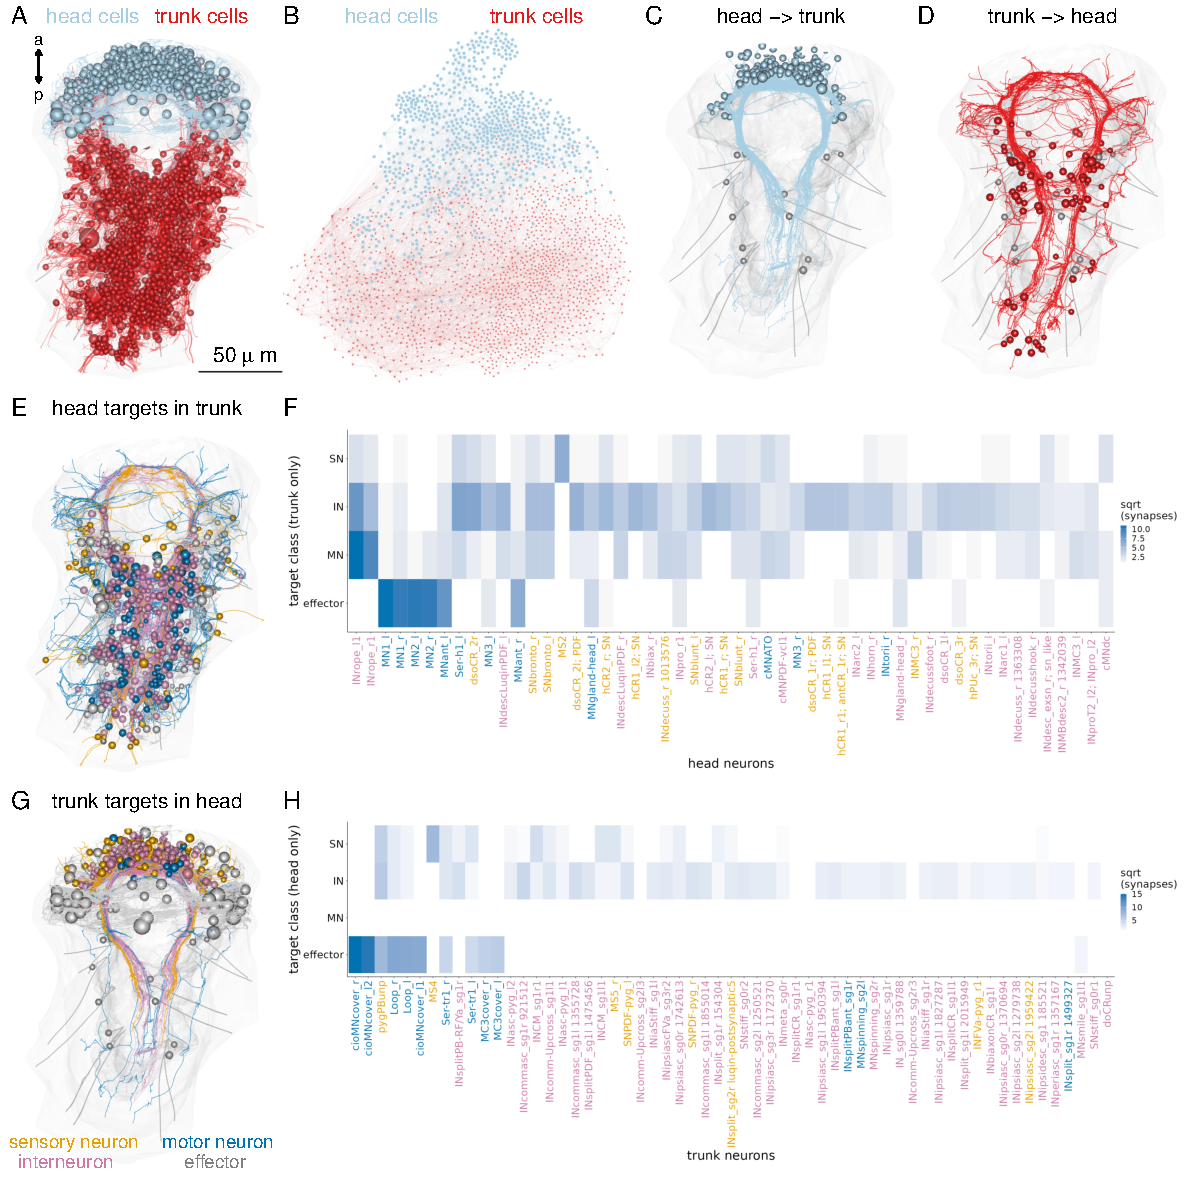
\includegraphics[width=1\textwidth,height=\textheight]{Figures/Figure10.png}

}

\caption{\textbf{Figure 10. Connections between the head and the trunk.
} (A) Morphological rendering of head (cyan) and trunk (red) cells,
which are part of the connectome. (B) Connectome graph with head (cyan)
and trunk (red) cells coloured separately. (C) Morphological rendering
of all head neurons with descending projections into the ventral nerve
cord. (D) Morphological rendering of all trunk neurons with ascending
projections into the head. (E) Morphological rendering of all synaptic
targets of head neurons in the trunk coloured by cell class. (F)
Distribution across classes of trunk targets of head neurons ordered by
the number of head to trunk synapses (top 50 neurons shown). (G)
Morphological rendering of all synaptic targets of trunk neurons in the
head coloured by cell class. (H) Distribution across classes of head
targets of trunk neurons ordered by the number of trunk to head synapses
(top 50 neurons shown). Figure 10---source data 1. Source data for panel
F. Figure 10---source data 2. Source data for panel H.}

\end{figure}%

\subsubsection{Intersegmental
connectivity}\label{intersegmental-connectivity}

Next, we analysed the neuronal complement and interconnectivity of the
body segments.

The three-day-old larva has three main trunk segments with
chaeta-bearing parapodia (chaetigerous segments) and a more anterior
cryptic segment (Steinmetz et al., 2011). In addition, the pygidium
forms the posterior-most part of the body (Starunov et al., 2015)
(Figure 1A, Figure 11A). The ciliary bands mark the posterior segment
boundaries.

\begin{figure}[H]

{\centering 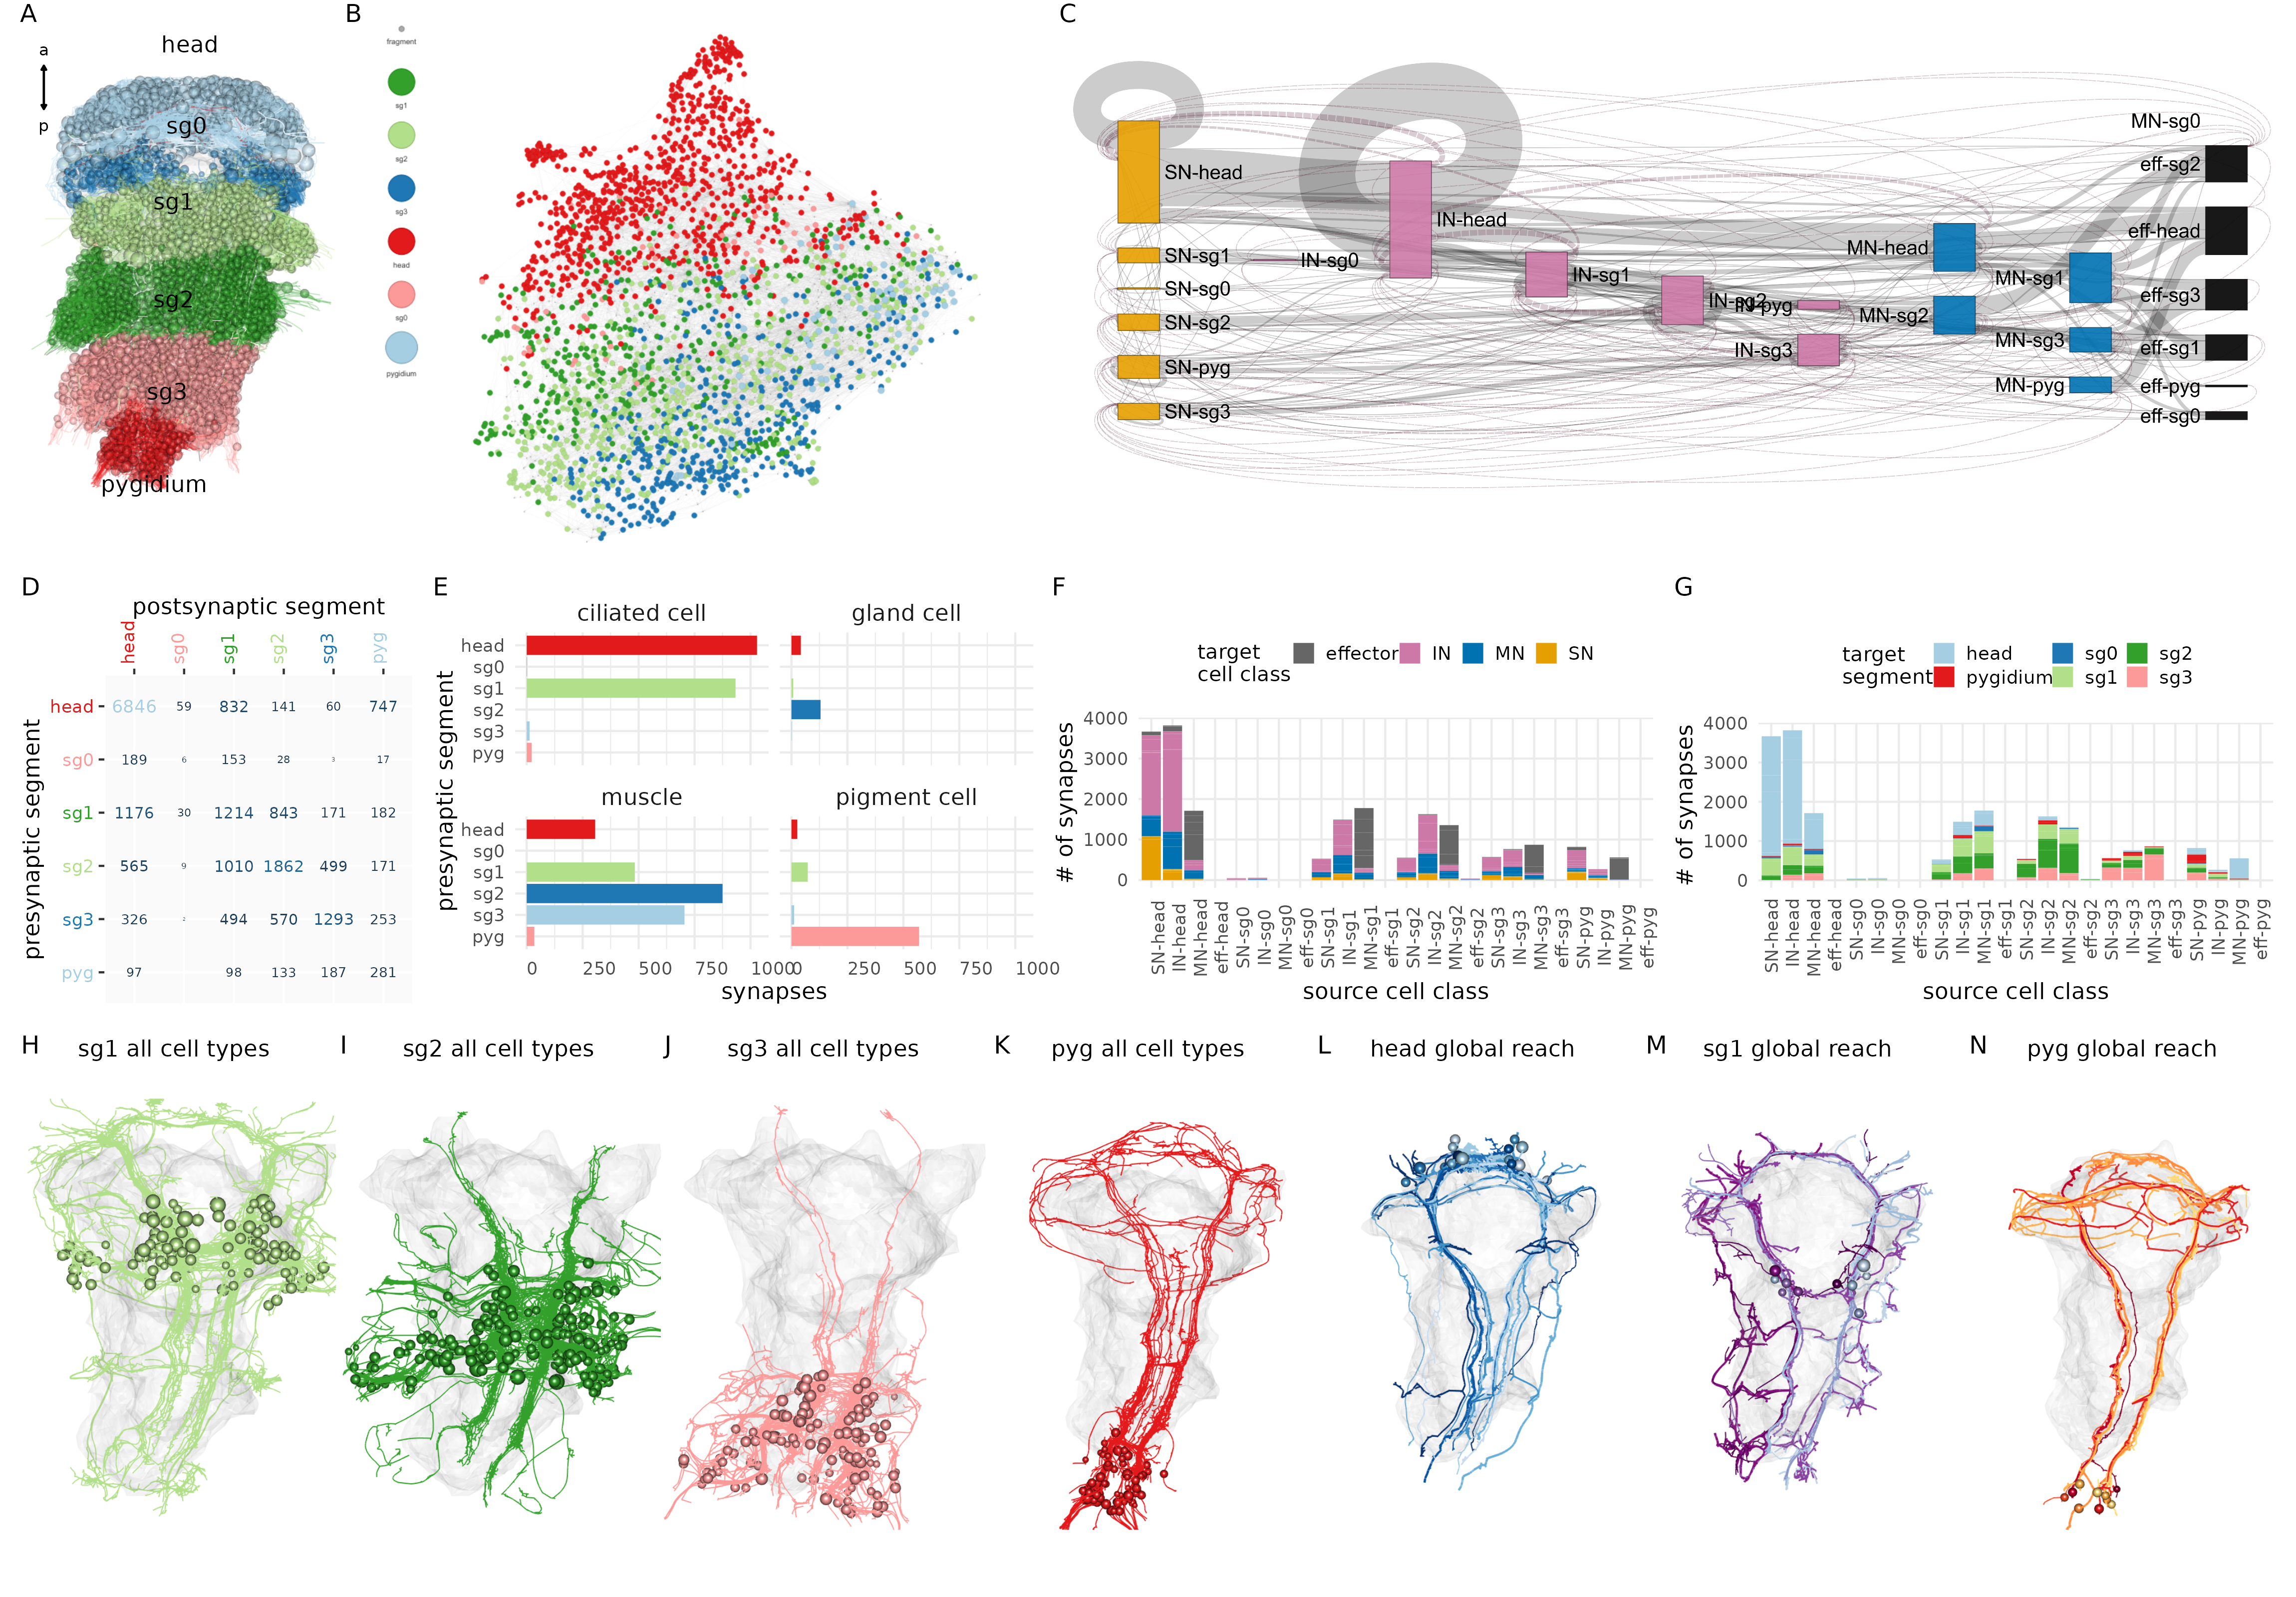
\includegraphics[width=1\textwidth,height=\textheight]{Figures/Figure11.png}

}

\caption{\textbf{Figure 11. Intersegmental connectivity in the larva }
(A) All cells in the body, coloured by body region. (B) Connectome graph
with nodes coloured by segment. (C) Sankey connectivity diagram of
sensory (orange), interneurons (cyan), motoneurons (blue) and effectors
(purple) in the different body regions. Edge thickness is proportional
to the number of synaptic connections. (D) Number of synaptic
connections linking the six body regions. (E) (F) Distribution of
synapses across different target cell classes for every source cell
class (SN, IN, MN, grouped by body region). (G) Distribution of synapses
across target body regions for every source cell class (SN, IN, MN,
grouped by body region). (H-K) Morphological rendering of all neuronal
cell types in segments 1-3 and the pygidium showing cross-segmental
neurite projections. (L-N) Neurons with global (whole-body) projections
in the head (L), first segment (M) and the pygidium (N). In (H-N) the
yolk outline is shown in grey for reference. Figure 11---source data 1.
Source data for panel B and C.Figure 11---source data 2. Source data for
panel D.Figure 11---source data 3. Source data for panel E.Figure
11---source data 4. Source data for panel F and G.}

\end{figure}%

Breaking down connections to segments (head, sg0-3, pygidium) or to cell
classes (SN, IN, MN, effector) and segments shows that the strongest
connections are formed within segments but there are also connections
between any pair of segments with the exception of segment 0 (Figure
11B-D, F, G; Figure 11---figure supplement 1). Segment 1 interneurons,
for example, connect to cells in four other body regions (Figure 11G).
In agreement with this, morphological rendering of cells per segment
reveals long-range projections beyond the boundary of each segment
(Figure 11H-K). The head, segment 1 and the pygidium all contain neurons
that project along the entire length of the body (neurons with `global
reach')(Figure 11L-N).

The innervation of different effector classes shows segment-selectivity.
Ciliary band cells receive most of their innervation from the head and
first segment (Figure 11E). Gland cells receive most of their synapses
from the second segment. Muscles are innervated by motoneurons with
somas in the head and segments 1-3. In contrast, pigment cells receive
their inputs predominantly from pygidial neurons (Figure 11E).

Overall, intersegmental connectivity is a hallmark of the
\emph{Platynereis} larval nervous system and suggests that motor control
and behaviour cannot be understood by focusing on a single segment or
the brain alone.

\subsubsection{Segment-specific cell types and circuits in the
trunk}\label{segment-specific-cell-types-and-circuits-in-the-trunk}

We identified many trunk-specific and segment-specific neuron types and
neuron types present in different subsets of segments (Figure 12, Figure
12---figure supplement 1-3), revealing a heteromeric organisation of the
annelid larval trunk. There are 10 neuronal cell types specific to the
first segment, eight to the second segment, two to the third segment and
seven to the pygidium (Figure 12, Figure 12---figure supplement 3).

These distinct sets of neurons suggest a functional specialisation of
the different trunk segments and are in agreement with segmental
differences in the expression of developmental transcription factors
(Vergara et al., 2017).

\begin{figure}[H]

{\centering 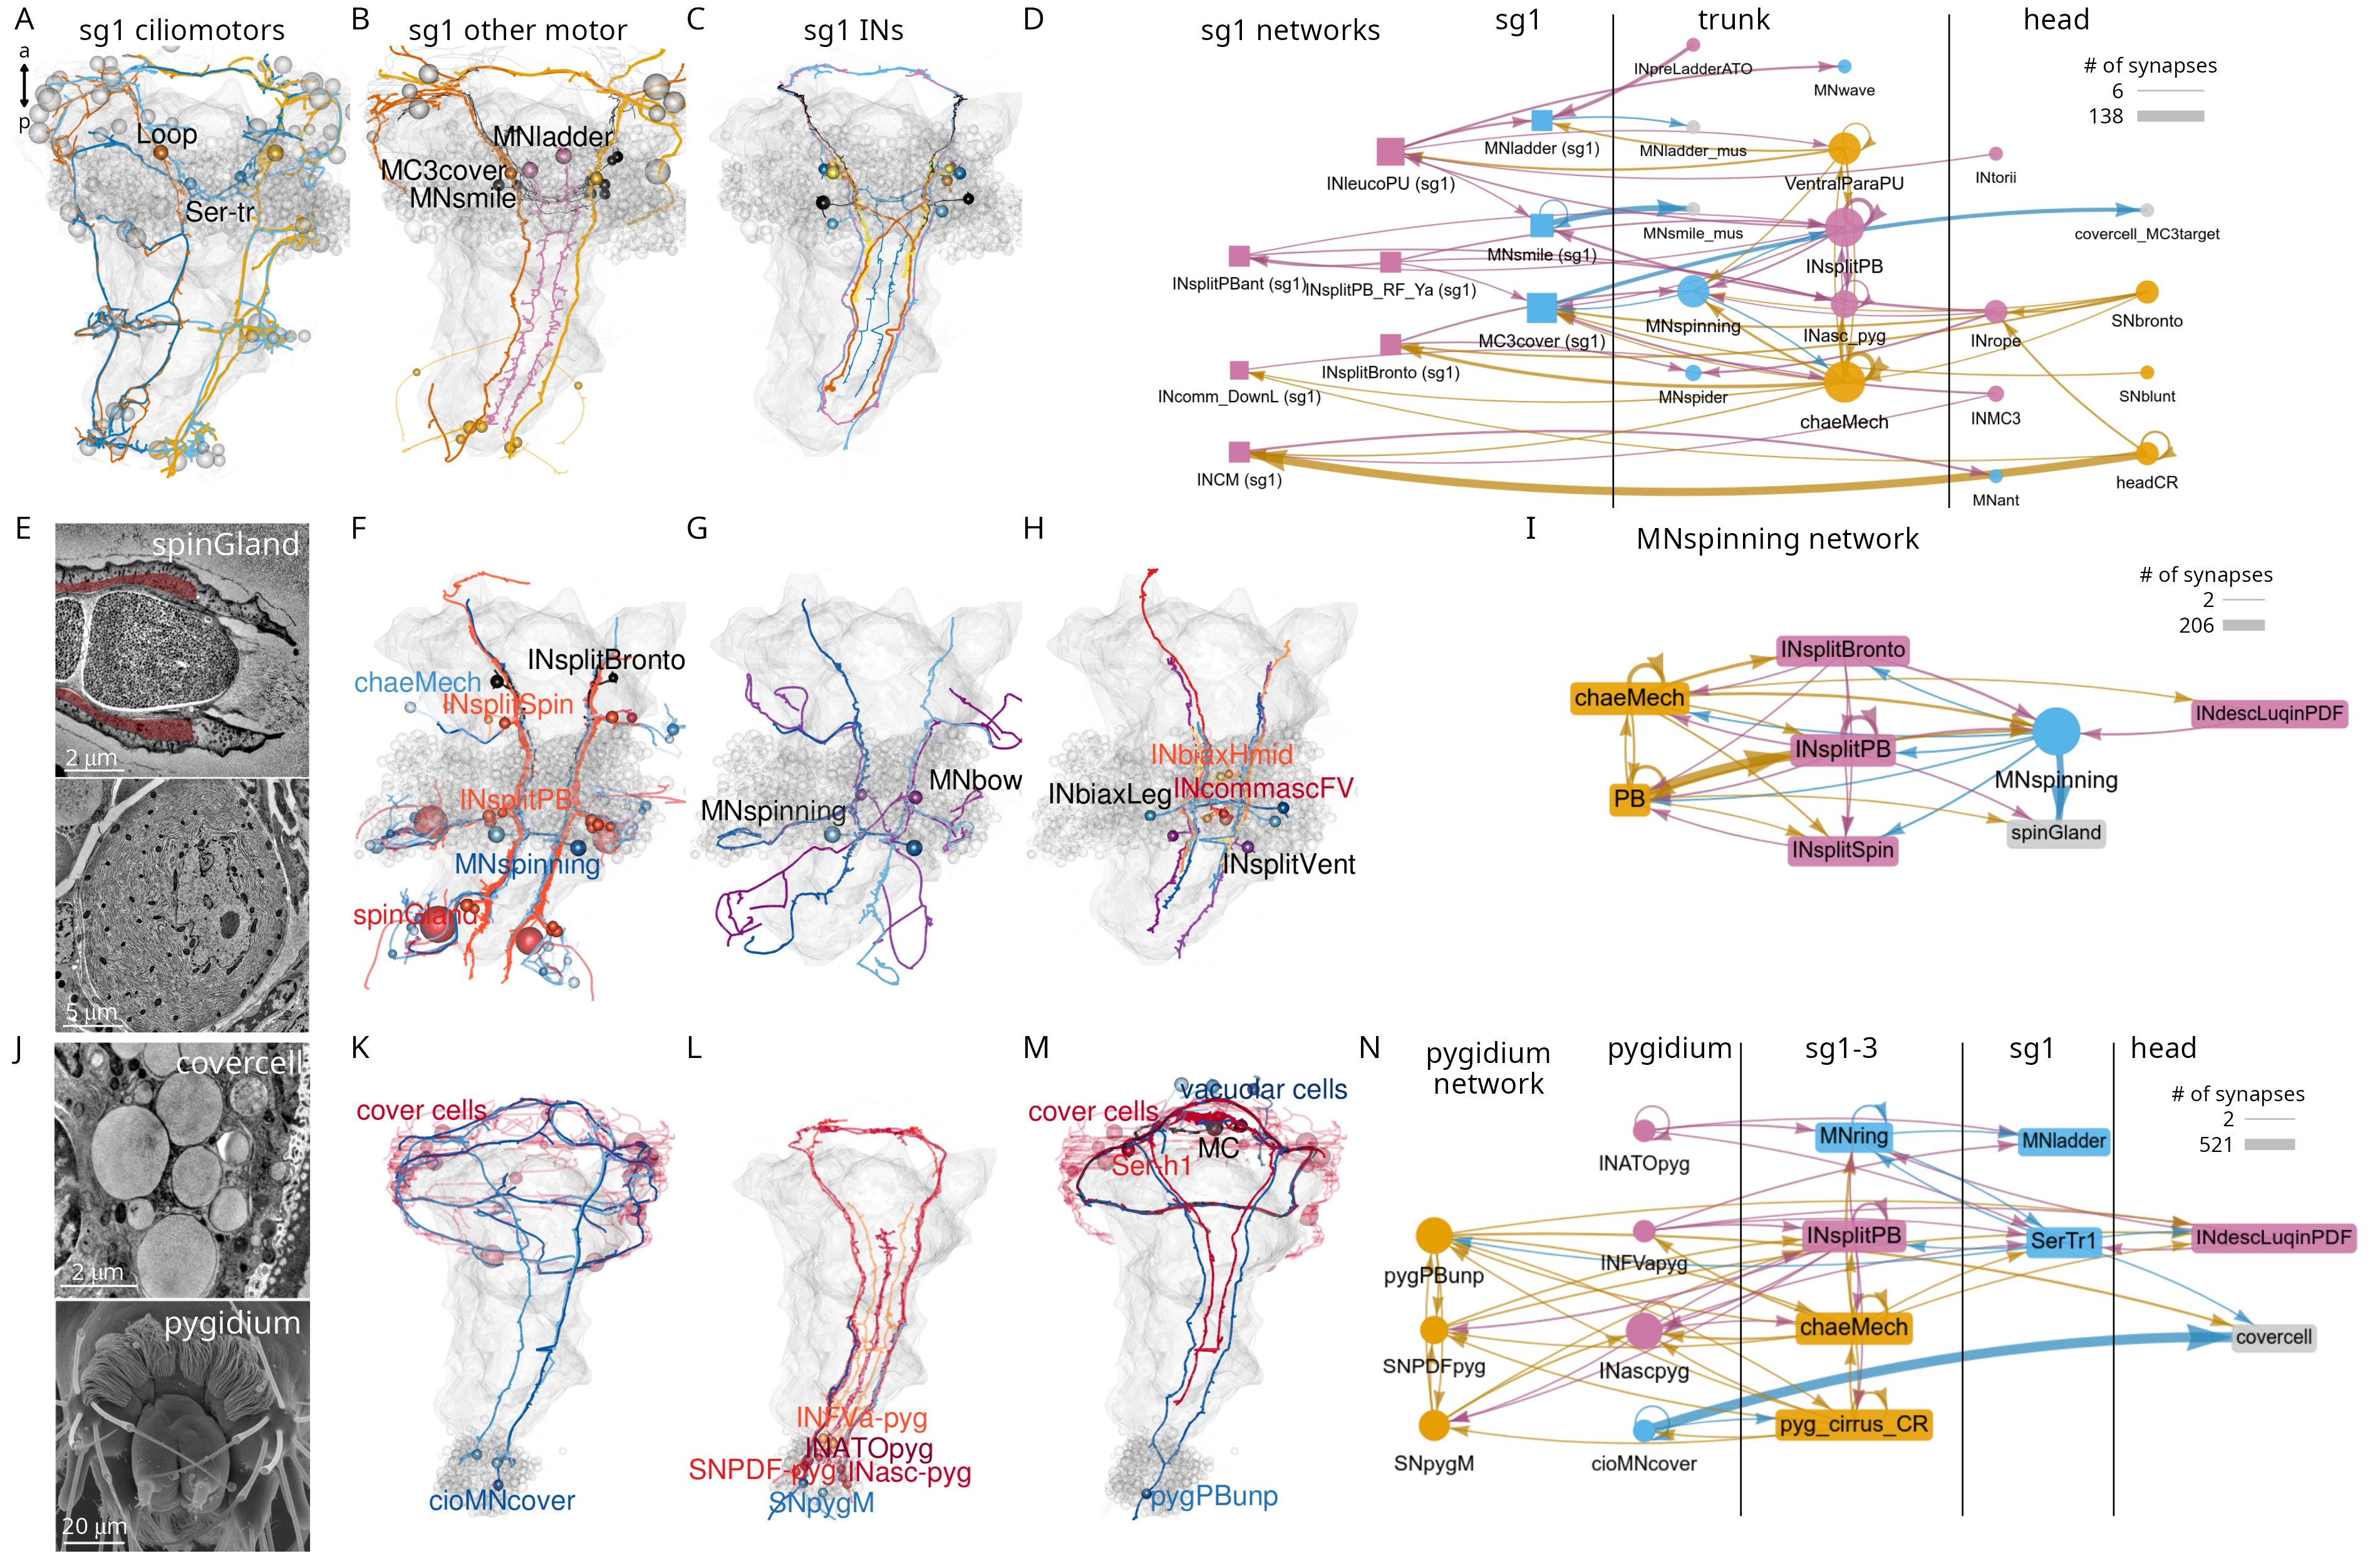
\includegraphics[width=1\textwidth,height=\textheight]{Figures/Figure12.png}

}

\caption{\textbf{Figure 12. Segment-specific circuits} (A) Morphological
rendering of segment-1-specific ciliomotor neurons. (B) Other
segment-1-specific motoneurons. (C) Segment-1-specific interneurons. (D)
Grouped connectivity graph of segment-1-specific cell types and their
synaptic partners in other trunk segments and the head. (E) Transmission
electron micrograph (TEM) of the spinGland nozzle and a secretory
vesicle. (F) The MNspinning motoneurons with their spinGland targets and
presynaptic partners. (G) The segment-2-specific MNspining and MNbox
motoneurons. (H) Segment-2-specific interneurons. (I) Grouped
connectivity graph of segment-2-specific cell types and their synaptic
partners. (J) TEM image of a cover cell covering the prototroch ciliary
band (top) and SEM image of the pygidium. (K) The pygidium-specific
cioMNcover cells and their cover cell targets. (L) Pygidium-specific
sensory and interneurons. (M) The pygidium-specific pygPBunp sensory
neuron and its targets in the head. (N) Grouped connectivity graph of
pygidium-specific neurons and their synaptic partners in the trunk and
head. Figure 12---source data 1. Connectivity matrix for the network in
panel D. Figure 12---source data 2. Connectivity matrix for the network
in panel I. Figure 12---source data 3. Connectivity matrix for the
network in panel N.}

\end{figure}%

The segment-specific cell types form unique motor circuits. The first
segment contains ciliomotor neurons involved in body-wide ciliary
closures and beating (Figure 12) (Verasztó et al., 2017).

In addition, segment-1-specific inter- and motoneurons have extensive
connections with other trunk and head cell types (Figure 12D), including
sensory inputs and motor outputs.

Segment 2 contains a unique pair of giant motoneurons (MNspinning) that
extensively innervate the contralateral spinning glands (spinGland) in
the second and third segments (Figure 12E, F). The four spinGland cells
have a large microvillar secretory pore at the tip of the ventral
parapodia (neuropodia). MNspinning cells form reciprocal connections
with pseudounipolar INsplit mechanosensory interneurons (Figure 12I).
Segment 2 also contains the large contra- and ipsilaterally projecting
MNbow motoneurons and four types of unique interneurons (Figure 12G, H).

The pygidium (Figure 12J) contains several unique cell types with global
reach (Figure 12---figure supplement 3). The cioMNcover and pygPBunp
motoneurons innervate the head cover cells (with large pigment vacuoles)
that occur in two rings anterior and posterior to the head protoroch
ciliary band (Figure 12J, K). The pygPBunp neuron also synapses on
another head pigmented cell type (vacuolar-cell). Pygidial cells also
form connections with segment 1-3 sensory, inter- and motoneurons.

Ranking trunk and pygidial cell types by various network centrality
measures often identified segment-specific cells as strongly connected
(e.g.~pygPBunp, Ser-tr1, Loop)(Figure 12---figure supplement 2).

\subsubsection{Serially repeated cells across the body
segments}\label{serially-repeated-cells-across-the-body-segments}

The whole-body connectome allowed us to systematically investigate the
occurrence of serially repeated cell types or cell-type families in the
annelid body.

Each larval segment has a distinct neuron-type composition with some
unique cell types (Figure 12). At the same time, several neuron types
occur in all chaetigerous segments. These include the chaeMech sensory
neurons (Figure 15A), the INsplitPB (Figure 16B) and INbackcross
interneurons and the MNche and MNhose motoneurons (not shown).

Four cell-type families (CR, PU, PB, INsplit) and two muscle types
(MUSlongV, MUStrans) occur across five or six body regions (head,
segments 0-3 and pygidium)(Figure 13). This pattern may indicate serial
homology, suggesting a metameric evolutionary origin for the trunk
segments, the pygidium and the head.

\begin{figure}[H]

{\centering \includegraphics[width=1\textwidth,height=\textheight]{Figures/Figure13.png}

}

\caption{\textbf{Figure 13. Serially homologous cell types.} (A)
Morphological rendering of all collar receptor (CR) neurons coloured by
segment. (B) All penetrating uniciliated (PU) neurons coloured by body
segment. (C)) All penetrating biciliated (PB) neurons coloured by body
segment. (D) All INsplit neurons coloured by body segment. (E) All
ventral longitudinal muscles coloured by body segment. (F) All
transverse muscles coloured by body segment. (G) All segmentally
iterated cell classes in ventral view. (H) Number of cells per body
segment for the six segmentally iterated cell types or cell-type
families. In (A-G) the yolk outline, the stomodeum, the aciculae and the
neuropil of the mechanosensory girdle are shown in grey for reference.}

\end{figure}%

\subsubsection{The mechanosensory
girdle}\label{the-mechanosensory-girdle}

The mechanosensory neurons and their postsynaptic partners form an
anatomically distinct system that spans the entire body of the larva.
Based on its morphology with a circumoral ring that continues in two VNC
tracts, we termed this system the mechanosensory girdle (Figure 14;
Figure 14---figure supplement 1; Video 4).

The girdle includes the penetrating vibration-sensing collar receptor
(CR) neurons (Bezares-Calderón et al., 2018), the penetrating biciliated
(PB) neurons, the penetrating uniciliated (PU) neurons, the
interparapodial penetrating multiciliated (interparaPM) neurons (Video
5). These penetrating cells all have one or more penetrating sensory
cilia surrounded by a collar of microvilli. The CR and PB neurons
express the mechanosensory polycystin PKD2-1, with CRs also expressing
PKD1-1 (Bezares-Calderón et al., 2018). The girdle also includes the
chaeMech dendritic cells that are chaetal mechanoreceptors (Figure 15
and see below).

The global projections of two mechanosensory interneuron types ---
INsplitPBant and INsplitPB-RF/Ya --- outline the axon tracts of the
mechanosensory girdle (Video 4; Figure 14---figure supplement 1).

The projections of several other neurons follow this axonal tract and
form a bundle at the ventral side of the VNC (Figure 14---figure
supplement 2).

The analysis of axon tracts and connectivity allowed us to identify
further sensory cell types that are part of the mechanosensory girdle.
These include the head SNbronto (dendritic), SNblunt (blunt sensory
ending beneath the cuticle, no cilium), and the pygidial SNPDF-pyg and
SNpygM cell types (Figure 14---figure supplement 1).

The interneurons in the girdle include various INsplit cells (see below)
as well as the pygidial ascending INasc-pyg and the head descending
INrope neurons (Bezares-Calderón et al., 2018) (Figure 14---figure
supplement 1).

The ciliomotor neurons MNant (Verasztó et al., 2017) (Figure 6G) and the
cover-cell motoneurons MC3cover (Figure 12B) are also part of the
girdle.

Overall, the anatomy and connectivity suggest that the girdle forms a
separate VNC tract for the processing of mechanosensory signals (Figure
14---figure supplement 2).

\begin{figure}[H]

{\centering \includegraphics[width=1\textwidth,height=\textheight]{Figures/Figure14.png}

}

\caption{\textbf{Figure 14. The mechanosensory girdle.} (A) The
connectome graph with cells of the mechanosensory girdle highlighted.
(B-C) All cells of the mechanosensory girdle in ventral (B) and lateral
(C) views. (D) Sensory neurons of the mechanosensory girdle. (E-F)
Interneurons of the mechanosensory girdle in anterior (E), ventral (F),
and lateral (G) views. (H) Motoneurons of the mechanosensory girdle. In
(B-H) the yolk outline, the stomodeum and the hindgut cells are shown in
grey for reference. In (E) the visual eye photoreceptors are also shown
in grey.}

\end{figure}%

\subsubsection{Chaetal mechanoreceptors}\label{chaetal-mechanoreceptors}

The trunk neurons with the largest number of postsynaptic partners and
the highest weighted degree in the grouped connectome are the chaeMech
chaetal mechanoreceptor neurons (Figure 12---figure supplement 1).

The chaeMechs are part of the mechanosensory girdle and are dendritic
sensory cells in segments 1-3 in both the dorsal (notopodium) and the
ventral (neuropodium) lobes of the parapodia (Video 5). The sensory
dendrites of chaeMech cells branch between the chaetal sacs (Figure
15A-D) and may sense the displacement of the chaetae during crawling
(proprioception) or due to external mechanical stimuli. The annelids
\emph{Harmothoë} (a polynoid) and \emph{Nereis} (a nereid) have cells
with a similar morphology called bristle receptors. These cells show
rapidly adapting spikes upon the displacement of the chaetae (Dorsett,
1964; Horridge, 1963). The chaeMech cells are also reminiscent of
dendritic proprioceptors in \emph{Drosophila} larvae that sense
body-wall deformations and provide feedback about body position through
premotor neurons (He et al., 2019; Vaadia et al., 2019; Zarin et al.,
2019). In \emph{Harmothoë} and \emph{Nereis}, the bristle receptors
connect to the giant axon system. In \emph{Platynereis}, chaeMech
neurons are highly interconnected. They project into the VNC where
inputs and output are mixed on the chaeMech axons (Figure 15B).

The direct postsynaptic partners of chaeMech cells include the premotor
interneurons INsplitCR, INsplitBronto, INchaeMech and the MNring and
MNspinning motoneurons (Figure 15E, F). The innervation of MNspinning by
chaeMech (and also indirectly by PB mechanosensory neurons; Figure 12I)
suggests that parapodial mechanosensation may regulate glandular
secretion of the spinGlands.

Among the direct targets of chaeMech neurons, the INsplitCR interneurons
receive the largest number of chaeMech synapses (Figure 15E). These
neurons are also postsynaptic to the collar receptors (CR) that mediate
a hydrodynamic startle response characterised by parapodial elevation
and the extension of the chaetae (Bezares-Calderón et al., 2018). At the
same time chaeMech do not or only weakly synapse on INrope and INCM
neurons, which are one of the main targets of CRs and INchaeMech neurons
lack synaptic inputs from CRs. This shows that the postsynaptic circuits
of CRs and chaeMechs are only partially overlapping. The shared
innervation of INsplitCR by CRs and chaeMechs suggests that there may be
proprioceptive inhibitory feedback during the startle response provided
by chaeMechs through the INsplitCR cells.

\begin{figure}[H]

{\centering \includegraphics[width=1\textwidth,height=\textheight]{Figures/Figure15.png}

}

\caption{\textbf{Figure 15. Chaetal mechanosensors and their circuits.}
(A) Morphological rendering of chaeMech neurons, ventral view. (B)
Outgoing (red) and incoming (cyan) synapses of chaeMech neurons, ventral
view. The soma of the chaeMech cells is shown in grey. (C) Lateral view
of chaeMech neurons. (D) TEM image of the sensory dendrites of chaeMech
neurons (yellow highlight) surrounding the chaetae (red highlight). (E)
Grouped synaptic connectivity matrix of chaeMech, CR and SNbronto
neurons and their downstream targets. (F) Same connectivity information
as in (E) represented as a network. In (A-C) the yolk outline, stomodeum
and the mechanosensory girdle neuropil are shown in grey for reference.
In (A, C) the aciculae and chaetae are also shown. Figure 15---source
data 1. Connectivity matrix for the network in panels E, F.}

\end{figure}%

\subsubsection{Parallel and converging mechanosensory
circuits}\label{parallel-and-converging-mechanosensory-circuits}

The strongest postsynaptic partners of the diverse girdle mechanosensory
neurons are ipsilateral interneurons with a bifurcating projection
(presudounipolar morphology). This family of interneurons ---
collectively referred to as INsplit --- could be subdivided into several
distinct cell types (INsplitCR, INsplitPB, INsplitPBant,
INsplitPB-RF/Ya, INsplitPUh, INsplitBronto, INCM)(Figure
16A-H)(Bezares-Calderón et al., 2018).

INsplit neurons occur in all four trunk segments and in the head
(INsplitPUh) and the distinct types have unique synaptic connectivity.
PB and interparaPM neurons specifically target INsplitPB and represent
their main input (Figure 16B, E). SNbronto and chaeMech neurons both
synapse on the INsplitBronto interneurons (Figure 15E, F, Figure 16C),
which have no other major presynaptic partners. CR and chaeMech neurons
synapse on INsplitCR (Figure 16A) while CR neurons also target INCM
(Bezares-Calderón et al., 2018). Some head PU neurons synapse on
INsplitPUh (Figure 16D).

Among trunk neuron types, INsplitCR and INsplitPB cells are highly
ranked based on the number of pre- and postsynaptic partners, suggesting
an integrating function (Figure 12---figure supplement 2).

INsplit neurons are premotor neurons, with connections to several trunk
motoneuron types that in turn innervate glands, ciliated cells, muscles
and pigment cells (Figure 16I, Figure 16---figure supplement 1).
Mechanosensory neurons thus provide input to all effector systems in the
body.

\begin{figure}[H]

{\centering 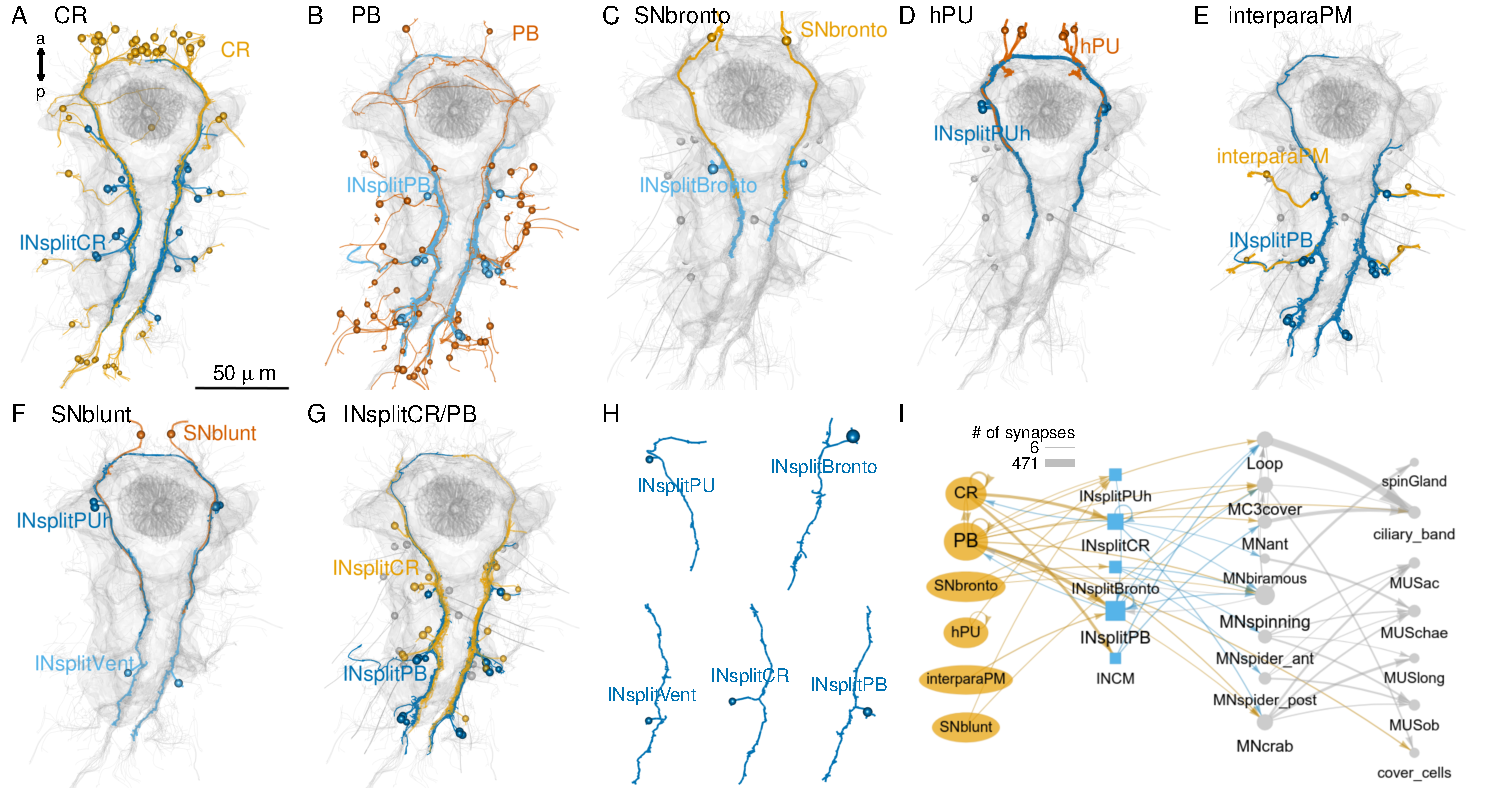
\includegraphics[width=1\textwidth,height=\textheight]{Figures/Figure16.png}

}

\caption{\textbf{Figure 16. Parallel systems of mechanosensory neurons
and their INsplit targets. } (A) Morphological rendering of all collar
receptor (CR) neurons and their INsplitCR targets. (B) All penetrating
biciliated (PB) neurons and their INsplitPB targets. (C) SNbronto
neurons and their INsplitBronto targets. (D) Head penetrating
uniciliated (hPU) neurons and their INsplitPUh targets. (E)
Interparapodial penetrating multiciliary (inerparaPM) neurons and their
INsplitPB targets. (F) SNblunt neurons and their INsplitPUh and
INsplitVent targets. (G) INsplitCR and INsplitPB neurons. (H) Example
morphologies of pseudounipolar INsplit neurons. Spheres represent the
position of cell somas. (I) Grouped connectivity diagram of the six
mechanosensory cell classes, their direct INsplit targets and downstream
motoneurons and effectors. Only connections with \textgreater5 synapses
are shown. In (A-G) the stomodeum, the aciculae and the yolk outline are
shown for reference. Figure 16---source data 1. Connectivity matrix for
the network in panel I.}

\end{figure}%

\section{Discussion}\label{discussion}

\subsubsection{\texorpdfstring{A whole-body resource for
\emph{Platynereis}}{A whole-body resource for Platynereis}}\label{a-whole-body-resource-for-platynereis}

Here we described a whole-body connectome for the segmented
three-day-old larva of the marine annelid \emph{Platynereis dumerilii}.
\emph{Platynereis} is the third species for which such a whole-body
resource is available, after \emph{C. elegans} and \emph{C.
intestinalis} (Cook et al., 2019; Ryan et al., 2016; White et al.,
1986). The power of such whole-body approaches lies in their
comprehensive nature encompassing not only the nervous system but also
all effectors and other cells. Overall, we identified, annotated and
spatially mapped 294 cell types and a total of 9,162 cells.

\emph{Platynereis} is distinguished from the nematode and tunicate
larval connectomes by the complexity of its nervous and effector
systems. The nervous system contains an order of magnitude more neurons.
The effector system is multi-modal, and includes muscles, locomotor
multiciliated cells, glands and pigment cells. The musculature is
composed of 53 distinct muscle cell-types, is segmental, and extends to
the parapodia that are supported by a chitin-based endoskeleton
(aciculae) (Jasek et al., 2022).

\subsubsection{Organisation of the
connectome}\label{organisation-of-the-connectome}

The overall organisation of the nervous system is feed-forward, with
information flow from a large diversity of sensors through interneurons
to effectors. Most sensory-motor connections are relatively shallow,
including direct sensory-motor neurons. However, we identified many
areas of recurrent connectivity suggesting internal processing beyond
sensory-motor arcs. One example is the ciliomotor system that is driven
by a rhythmic pacemaker circuit (Verasztó et al., 2017). The endogenous
activity generated by this circuit is modified by sensory inputs such as
hydrostatic pressure or UV light (Calderón et al., 2023; Jokura et al.,
2023).

We also identified several potential sites of multisensory integration
suggesting extensive cross-talk between distinct channels of sensory
processing. One experimentally characterised example is a cross-talk
between phototaxis and UV avoidance (Verasztó et al., 2018). We have now
found that the eyespot R1 and adult eye photoreceptors converge on the
INR interneurons (Figure 7G, H). This suggests a further layer of
integration of light-sensory pathways. The connectome now enables the
systematic identification of similar circuit motifs for sensory
cross-talk with predictive value.

The connectome also shows a modular organisation and can be subdivided
into functionally distinct sub-networks. These sub-networks are strongly
connected within themselves, but there are also extensive connections
between the modules. Such inter-module connections may establish a
hierarchy of behaviours e.g.~by cross-inhibition.

The mushroom bodies also show a parallel feed-forward organisation with
minimal feedback. This could be due to the developmental snapshot we
acquired for the three-day-old stage. Mushroom bodies grow in size and
form a morphologically clearly recognisable region only in later-stage
larvae and juveniles (Tomer et al., 2010). This growth is likely
accompanied by circuit maturation. However, we think that the mushroom
body cell types and circuits we reconstructed already show a functional
circuit architecture. The MB cell types and their connections show
left-right stereotypy and specificity of connectivity. It may be that
annelid mushroom bodies can support associative learning by this
multilayer perceptron-like organisation. In the cephalopods \emph{Sepia
officinalis} and \emph{Octopus vulgaris}, similar feedforward
information flow characterises the vertical lobe, a learning centre
(Shomrat et al., 2011). The circuitry here has a simple fan-out fan-in
architecture that in \emph{Octopus vulgaris} shows further
interconnections between the parallel feedforward networks (Bidel et
al., 2023). In \emph{Platynereis}, we only identified very weak
connections between the parallel networks, at the level of the MB
projection neurons.

\subsubsection{Functional predictions}\label{functional-predictions}

The connectome also enables the generation of specific circuit-level
hypotheses about neuronal control and integration in the
\emph{Platynereis} larva.

The analysis of the mechanosensory systems, for example, led to several
new functional predictions. The convergence of mechanosensory pathways
to the MNspinning motoneurons of the exocrine spinGlands indicates that
glandular secretion is regulated by mechanosensory inputs to the
parapodia. These circuits could regulate tube secretion by the benthic
juvenile worms.

We also identified a potential site of mechanosensory feedback that may
regulate the startle response. During a vibration-induced startle, the
parapodia and their chaetae are extended, potentially activating the
chaeMech chaetal mechanoreceptors. The chaeMech neurons synapse on the
INsplitCR cells that are also a main target of the vibration-sensing CR
neurons. An inhibitory signal from chaeMech to INsplitCR could lead to
the controlled cessation of a startle.

By comprehensive tracing and cell annotation, we also identified a
unique class of pigment-motor neurons (MC3cover, cioMNcover, pygPBunp).
The direct synaptic innervation of pigment cells suggests that
pigmentation may be under neuronal control in \emph{Platynereis} larvae.
We do not know how neuronal inputs may influence pigment cells. One
possibility is that synaptic signals induce the movement or bleaching of
the pigment vacuoles. In the cover cells, we occasionally observed the
rapid disappearance of the pigment granules. The fact that at least one
of the pigment-motor cells (pygPBunp) is also directly mechanosensory
(Bezares-Calderón et al., 2018) suggests that mechanical cues may alter
pigmentation.

Network analysis also identified various hub neurons of potential
functional importance. For example, in the brain, INRGWa and INW
interneurons integrate a large number of inputs. Likewise, in the trunk
mechanosensory system, INsplitCR and INsplitPB neurons receive many
distinct inputs. Multi-pathway convergence can occur both at the level
of interneurons and on motoneurons (e.g.~MNant, vMN, MNspinning).

\subsubsection{Circuits for whole-body
coordination}\label{circuits-for-whole-body-coordination}

The \emph{Platynereis} whole-body connectome resource highlights the
value of having access to comprehensive circuit and cell-type
information. In the \emph{Platynereis} larva, almost every functional
module spans several body regions and often the entire body.

The coordinated closure and beating of cilia along the body segments is
ensured by giant ciliomotor neurons that innervate target cells in
multiple segments (Verasztó et al., 2017). The secretion of spinGlands
across segments is likely also coordinated since the two MNspinning
neurons innervate the four spinning glands in segments 2 and 3. Among
the muscle motoneurons, the vMNs MN1 and MN2 innervate ventral and
dorsal longitudinal muscles (MUSlong) in each segment. MNspider cells
synapse on contralateral muscles in two consecutive segments and the
muscle targets of MNcrab and MNbow neurons span three segments
(Bezares-Calderón et al., 2018). In the pigment-motor system, the
cioMNcover cells each innervate half the ring of the cover cells and
pygPBunp innervates the entire ring, also suggesting coordinated
regulation.

Intersegmental coordination is also apparent at the level of sensory and
interneurons. For example, individual chaeMech cells can synapse on
interneurons in three segments. INrope and INchaeMech interneurons
target motoneurons across three segments, INsplitCRATO, INsplitBronto
and INsplitVent in two segments. The globally reaching INsplitPBant
cells have postsynaptic partners in all four segments and the pygidium.

These examples demonstrate the importance of a whole-body approach in
connectomics to understanding circuit function and behaviour. Partial
connectomes could not deliver satisfactory circuit explanations for any
of these systems We do not expect this to be different for other
animals.

\subsubsection{Circuit evolution by duplication and
divergence}\label{circuit-evolution-by-duplication-and-divergence}

An exciting perspective in connectomics is to learn about circuit
evolution by the analysis of comprehensive datasets that integrate
anatomy and connectivity. Our reconstructions identified a potential
case for circuit evolution by duplication and divergence of synaptically
connected cell types (Tosches, 2017).

The mechanosensory girdle contains several morphologically similar
mechanosensory neurons bearing penetrating cilia at the tip of their
sensory dendrites (PB, CR, interparaPM, PU and pygPBunp). These cells
likely represent evolutionarily related sister cell types (Arendt,
2008). Some of these neurons also show overlapping gene regulatory
signatures --- supporting their classification as sister cell types ---
as they all can be labelled by the same \emph{PKD2-1} transgene (PB, CR
and pygPBunp)(Bezares-Calderón et al., 2018).

These mechanosensory neurons synapse on distinct subsets of INsplit
types. Based on their morphological similarity, INsplit cells are also
likely related among themselves.

This pattern suggests that these parallel systems may have evolved
through the process of circuit duplication and divergence. According to
this model, the diversification of mechanoreceptors may have been
paralleled by the diversification of their postsynaptic INsplit neurons.
This enabled sensory refinement in parallel with the evolution of
matched downstream circuits and behaviours.

The duplication and divergence of cell-type sets also characterised the
evolution of the vertebrate cerebellum (Kebschull et al., 2020). Further
support for this model in \emph{Platynereis} could come from
comprehensive gene expression analyses for the distinct mechanosensory
and INsplit neurons.

\subsubsection{Connectomics informs the evolution of the annelid
segmental body
plan}\label{connectomics-informs-the-evolution-of-the-annelid-segmental-body-plan}

Our dataset represents, to our knowledge, the first whole-body
connectome of a segmented animal. These data also inform our
understanding of the evolution of the annelid body segments and nervous
system, both long-standing questions in evolution and development
(Balfour, 1881; Nielsen et al., 2018; Nielsen, 2005; Sedgwick, 1884;
Starunov et al., 2015; Steinmetz et al., 2011).

By mapping cell-type distributions across segments we found evidence for
segmental homology overlain by a heteromeric pattern with
segment-specific cell types. The serial homology of the cryptic segment
(sg0) with the other three trunk segments (sg1-3) (Steinmetz et al.,
2011) is confirmed by neuron and muscle types shared between these four
segments. In addition, the pygidium and the head may have metameric
origin. The pygidium has a coelomic cavity and muscle cell types
(MUSlong, MUStrans) shared with the other trunk segments (Jasek et al.,
2022; Starunov et al., 2015). The segmental origin of the annelid head
is suggested by a Cambrian annelid fossil where the head is formed by a
segment with parapodia and chaetae (Parry et al., 2015).

The metameric origin of all six body regions receives additional support
from our connectome reconstructions. We identified muscle cell types
(MUSlongV, MUStrans), sensory neuron types (CR, PB, PU) and one family
of interneurons (INsplit) shared by five or six of the body regions. One
interpretation of this pattern is that the annelid body evolved from an
organisation with six homomeric regions that subsequently diversified
but retained a core set of homologous cells. Further tests of this model
could come from future whole-body connectomes of other annelid species.

The identification of a mechanosensory girdle in \emph{Platynereis}
reminded us of another classic hypothesis about bilaterian body-plan
evolution.

In 1881, Francis Balfour put forward the hypothesis that the ancestral
nervous system from which the nervous system of arthropods, molluscs and
other invertebrates derived was ``a circumoral ring, like that of
Medusae, with which radially-arranged sense-organs may have been
connected''. He posits a transition scenario in which a ``circumoral
nerve-ring, if longitudinally extended, might give rise to a pair of
nerve-cords united in front and behind'' (Balfour, 1881).

In 1884, Sedgwick further developed this model and derived the
bilaterian mouth and anus through the fusion of the lateral lips of the
gastric slit of a radially symmetric animal (Sedgwick, 1884). Metameric
segmentation in this model evolved from the mesenteries and somites from
gut pouches of a radial ancestor. For a thorough modern treatment of
this Balfour-Sedgwick model --- also referred to as the amphistomy
theory --- see (Nielsen et al., 2018).

Our connectome reconstructions in the \emph{Platynereis} larva are
compatible with the Balfour-Sedgwick theory. The mechanosensory girdle
looping around all six homologous body segments can be interpreted as a
derivative of a circumoral nerve ring looping around homomeric body
regions. The girdle could correspond to radially-arranged mechanosensory
organs around the cnidarian oral opening (e.g. (Singla, 1975)) (Figure
17). Alternative transition scenarios, such as the evolution of a new
opening at the aboral pole of a radial ancestor and de-novo evolution of
a mechanosensory, circumoral nerve ring seem less plausible.

\begin{figure}[H]

{\centering \includegraphics[width=1\textwidth,height=\textheight]{Figures/Figure17.png}

}

\caption{\textbf{Figure 17. Origin of the mechanosensory girdle by
amphistomy?} Hypothetical homology of the circumoral nervous system in a
radially symmetrical ancestor of bilaterians and the mechanosensory
girdle.}

\end{figure}%

Testing this model would require detailed reconstructions of cnidarian
circumoral nervous systems. We predict that there may be bifurcating
interneurons in cnidarians that are postsynaptic to circumoral
mechanosensors and project in two directions along the oral opening
(similar to INsplit neurons).

\section{Acknowledgments}\label{acknowledgments}

This research was funded by a Wellcome Trust Investigator Award
214337/Z/18/Z. The research has also been supported by a grant from the
Deutsche Forschungsgemeinschaft (JE 777/3---1). This project has
received funding from the European Research Council (ERC) under the
European Union's Horizon 2020 research and innovation programme (grant
agreement No 101020792). We thank Nobuo Ueda, Nadine Randel, James David
Beard, and Sara Mendes for contributing to tracing and Konrad Heinz for
helping to implement an R workflow with the Natverse package. We thank
Tom Kazimiers for support with the realignment of the stack.

\section{Materials and Methods}\label{materials-and-methods}

\textbf{Data and code availability}

The EM image stack with all traces and annotations are available at
\url{https://catmaid.jekelylab.ex.ac.uk} and can be queried in CATMAID
or via the CATMAID application programming interface (API) with the
catmaid/natverse packages (Bates et al., 2020). The dataset includes all
EM images (in jpg format), skeletons, meshes, node tags, connectors
(both synapses and desmosomes) and annotations. We also provide all the
R scripts we used for data retrieval and the generation of the figures
(Jékely et al., 2024). All plots, diagrams (including anatomical
renderings), figure layouts should be fully reproducible by using the R
scripts provided. Scripts were mostly organised by figure, except some
generalist scripts e.g.~to load libraries, CATMAID access data and
general functions (`Natverse\_functions\_and\_conn.R').

\textbf{Specimen preparation, transmission electron microscopy and image
processing}

Fixation and embedding were carried out on an 72 hpf \emph{Platynereis}
larva (HT9-4) as described previously (Conzelmann et al., 2013). Serial
sectioning and transmission electron microscopy were done as described
in (Shahidi et al., 2015). The section statistics for the HT9-4 (NAOMI)
specimen were previously described (Randel et al., 2015). The serial
sections were imaged on a FEI TECNAI Spirit transmission electron
microscope with an UltraScan 4000 4X4k digital camera using Digital
Micrograph acquisition software (Gatan Software Team Inc., Pleasanton)
and SerialEM (Schorb et al., 2019). The images for the HT9-4 projects
were scanned at various pixel resolutions: 5.7 nm/pixel, 3.7 nm/pixel,
and 2.2 nm/pixel. Images were stitched and alignment with TrakEM2
(Cardona et al., 2012).

We used the collaborative annotation toolkit CATMAID for tracing,
annotation and reviewing of skeleton annotations (Saalfeld et al., 2009;
Schneider-Mizell et al., 2016).

Due to contrast and focus problems in the main dataset we had to
re-image certain layers at higher resolutions, to allow tracing of
neurons. These re-imaged series were made into independent CATMAID
projects. This included five extra projects, taken at various points
throughout the main dataset. All layers including the information on
lost layers, immunogold labelling and re-imaging are listed in
Supplementary Table 2. The largest of these,
Plexus\_HT-4\_Naomi\_project\_\_372-4013, consisted of 1407 layers at
resolution of 2.2 nm. This stack mostly focused on the brain plexus and
the ventral nerve cord where most neurites and synapses occur. Other
projects consisted of three jump/gap regions that required not only high
resolution but also better realignment. One set contained all the
immunogold labelled layers (Shahidi et al., 2015) that were not included
in the main aligned dataset. These layers had very low contrast due to
the immunolabelling procedure and therefore required higher resolution
imaging. All projects were first created and processed in TrakEM2 and
then exported as flat jpeg images into CATMAID.

\textbf{Image-stack realignment and transformation of spatial data in
CATMAID}

To improve the traceability of the vEM stack in all areas, we realigned
the raw TEM images to improve the previously reported alignment of the
volume (Randel et al., 2015). First, we opened the original project with
the TrakEM2 plugin for FIJI (ImageJ) (version 2.0.0-rc-15/1.49k / Java
1.6.0\_24 (64-bit) -- 2014). We set the region of interest (ROI) to
width: 25792, height: 28800, x-shift: 20885, y-shift: 11928. All 4846
layers were then exported as flat TIFF images with a scale of 100\%,
8-bit grayscale, no background color (0). A new blank TrakEM2 project
was then created in FIJI and the exported TIFF images were imported
using the project import function ``import sequence as grid''. The
project was then aligned according to Albert Cardona's 2016 alignment
protocol
(https://wikis.utexas.edu/display/khlab/TrakEM2+elastic+alignment?preview=/139168916/194807990/TEM
Alignment in TrakEM2 (Cardona 2016).pdf) with some modifications. The
image filters were previously applied to the images, and therefore were
not required. First, an `Affine' alignment was applied using the
following parameters: least squares (linear feature correspondences)
mode, choosing entire layer range with first layer as reference, using
visible images only and no propagation, initial Gaussian blur of 1.6
pixels, 3 steps per scale octave, minimum image size of 64 pixels and
maximum of 2048 pixels, feature descriptor size of 8, feature descriptor
orientation bins of 8, closest ratio of 0.92, with clear cache selected,
feature extraction threads of 30, maximal alignment error of 100 pixels,
minimal inlier ratio of 0.20, minimal number of inliers of 12, expected
transformation as Affine, testing multiple hypotheses with tolerance of
5.00 pixels, testing maximal layer neighbour range of 5 layers, giving
up after 5 failures, desired transformation as Affine, regularizing
model, maximal iteration of 1000, maximal plateauwidth of 200,
regularizer as Rigid, and lambda of 0.10. Next, two iterations of
Elastic alignment were applied using the following parameters: block
matching layer scale of 0.05, search radius of 200 pixels, block radius
of 2000 pixels (increased to 2400 pixels during second iteration),
resolution of 60, correlation filters with minimal PMCC r of 0.10,
maximal curvature ratio of 1000, maximal second best r/best r of 0.90,
using local smoothness filter, with approximate local transformation as
Affine, local region sigma of 1000 pixels, absolute maximal local
displacement of 10 pixels, relative maximal local displacement of 3.00,
as pre-aligned layers, testing maximal of 4 layers, approximate
transformation as Rigid, maximal iterations of 1000, maximal plateau
width of 200, spring mesh stiffness of 0.01, maximal stretch of 2000
pixels, maximal iterations of 3000, maximal plateauwidth of 200, using
legacy optimizer. After each alignment procedure the project was saved
as an XML file with a different name. Finally, images were exported for
CATMAID using TrakEM2 in FIJI (version 2.0.0-rc-69/1.52p / Java
1.8.0\_172 (64-bit) -- 2019). After the realignment, the transformation
of all traced neuron skeletons in CATMAID was necessary to match the
newly applied image alignment transforms. To achieve this, we used a
logic script (Tom Kazimiers, Kazmos GmbH) that applied a realignment
transformation process from the TrakEM2 xml project file to the CATMAID
data. This script was added as a management command in CATMAID
(https://github.com/catmaid/CATMAID/blob/master/django/applications/catmaid/management/commands/catmaid\_update\_tracing\_data\_using\_trakem2\_xml.py).
When applied, these transformation offsets were within ±1 pixel accuracy
for all parented nodes. The code is available in the CATMAID GitHub
repository, commit e25debb
(https://github.com/catmaid/CATMAID/commit/e25debb).

\textbf{Neuron tracing, synapse annotation and reviewing}

To digitally reconstruct every neuron in the serial TEM dataset of the
three-day-old larva, we used the collaborative web application CATMAID
(Saalfeld et al., 2009; Schneider-Mizell et al., 2016) installed on a
local server.

The total construction time of all skeletons was over 2,970 hours with
an additional 782 hours of review time.

To mark the position of cell somas, we tagged the centre of each nucleus
in the volume. At the approximate centre of each nucleus, we changed the
radius of a single node according to the soma size in that layer. All
skeletons were rooted on the soma and the node was tagged with `soma'.

Ultrastructural features (number and orientation of microtubules,
electron density of the cytoplasm and vesicles, ER structure) and a high
resolution dataset of the neuropil and the ventral nerve cord aided
tracing through low-quality layers and gaps.

We identified synapses based on a vesicle cloud close to the plasma
membrane. Most synapses were visible in consecutive layers (for example
images see (Randel et al., 2014) and browse the data). We also checked
for the proximity of mitochondria in the same arbour in case of
ambiguous synapses --- a requirement supported by quantitative
connectomic data in \emph{Drosophila} (Schneider-Mizell et al., 2016).
The systematic review of all neurons belonging to a cell type was done
by one or multiple reviewers until close to 100\% was reached for every
cell. Cells were further checked in the 3D widget to split implausible
skeletons. Synapses were reviewed multiple times, from both the pre- and
postsynaptic arbour.

\textbf{Cell nomenclature and annotations}

All cells have a unique name. We named neurons based on their type
(e.g.~sensory or motor; SN, MN) cell body position (left or right, head
or trunk segment), axonal morphology, neuropeptide expression, and other
specialisations (e.g.~sensory morphology). Cells of the same type have
similar names, distinguished by body position indicators and numbers.
These indicators follow the general cell-type name separated by the
first \_ symbol in the name string. We endeavoured to give names that
were easy to remember. The name of many sensory neurons start with SN
followed by a specific term (e.g.~blunt, bronto, stiff). Interneurons
often start with IN and motoneurons with MN. There are exceptions,
including neurons with known function (e.g.~PRC for photoreceptor cells)
and neurons with prominent morphology (e.g.~Loop). Segmental position
(sg0-3) and body side (l or r) is indicated in the name of most neurons.
Non-neuronal cells were named based on anatomical terms
(e.g.~prototroch) or by abbreviations (e.g.~EC for epithelial cell).

All cells have multiple annotations, which can be used to query the
database in CATMAID or through the CATMAID API (e.g.~in R b the catmaid
package). Neurons belonging to a cell-type category were annotated with
the generalist annotation `celltype' and a cell-type-specific annotation
(e.g.~celltype23 for the INpreMN neurons). Non-neuronal cells belonging
to a cell-type category were annotated with the generalist annotation
`celltype\_non\_neuronal' and a cell-type-specific annotation
(e.g.~celltype\_non\_neuronal23 for the acicula cells). Neurons were
also annotated with descriptors of their projection morphologies
(e.g.~commissural, ipsilateral, pseudounipolar etc.), neuron class
(Sensory neuron, sensory-motor neuron, sensory-neurosecretory neuron,
interneuron, inter-motorneuron and motorneuron {[}note the `r', which we
kept for backward compatibility{]}). In CATMAID, we recommend the use of
regular expressions for searching annotations e.g.~\^{}motorneuron\$ to
retrieve exact matches. Differentiating neurons with immature sensory
dendrites or axonal projections with axonal growth cones and with no or
few synapses were annotated `immature neuron' (402 cells). Ascending
trunk neurons and descending head neurons traversing the
circumesophageal connectives were annotated `head-trunk'. Neurons with a
soma in the head and a descending decussating axon were annotated with
`decussating'. Cells were also annotated according to the location of
their soma in a certain body region (head --- as `episphere', trunk ---
as `torso', `pygidium'), body side (`left\_side', `right\_side'),
segment (`segment\_0' etc.), and germ layer (ecto-, meso-, endoderm).

\textbf{Criteria for including cells in the connectome}

When defining the connectome, we aimed at including differentiated cells
and skeletons connected with at least three synapses to the main graph.
We used the script `connectome\_from\_CATMAID.R' to derive the final
full connectome graph. First, we fetched all synaptic connectors and
their pre- and postsynaptoc partners. Each single synapse was assigned a
weight of one and edges connecting the same nodes in the same direction
were summed. We then removed all vertices from the graph with \textless3
synapses. We checked for connected components and selected the largest
subgraph.

\textbf{Network layout}

The layout of the full connectome was generated by force-field-based
clustering. We used the Force Atlas tool in Gephi 0.10.1 (Bastian et
al., 2009). The inertia was set to 0.1, repulsion strength was 35,
attraction strength was 10, maximum displacement was 5, gravity was 20,
speed was 5 and the attraction distribution option was on. The `auto
stabilise function' was off. Towards the end of the clustering the
`adjust by sizes' option was also selected. To prevent node overlap, we
then run the `Noverlap' function. Node positions from this Gephi layout
were imported and further graph manipulations (including node colouring)
were carried out in R.

\textbf{Network analysis}

We used CATMAID (several releases), Gephi 0.10.1 and R for network
analysis. For graph analysis and visualisation, we used R and the
iGraph, tidygraph, visNetwork and networkD3 packages (Allaire et al.,
2017; Almende et al., 2019; Csardi et al., 2006).

\textbf{Data analysis and plotting}

For data analysis, we used R and Rstudio (various releases)(Posit team,
2023). For data handling and plotting we endeavoured to adhere to the
practices and packages of the Tidyverse (Wickham et al., 2019). Data
plotting was done with the ggplot2 package (Wickham et al., 2016). See
also the `versionInfo.txt' and `sessionInfo.txt' files in the repository
for full package and version information.

\section{Figure supplements}\label{figure-supplements}

\begin{figure}[H]

{\centering 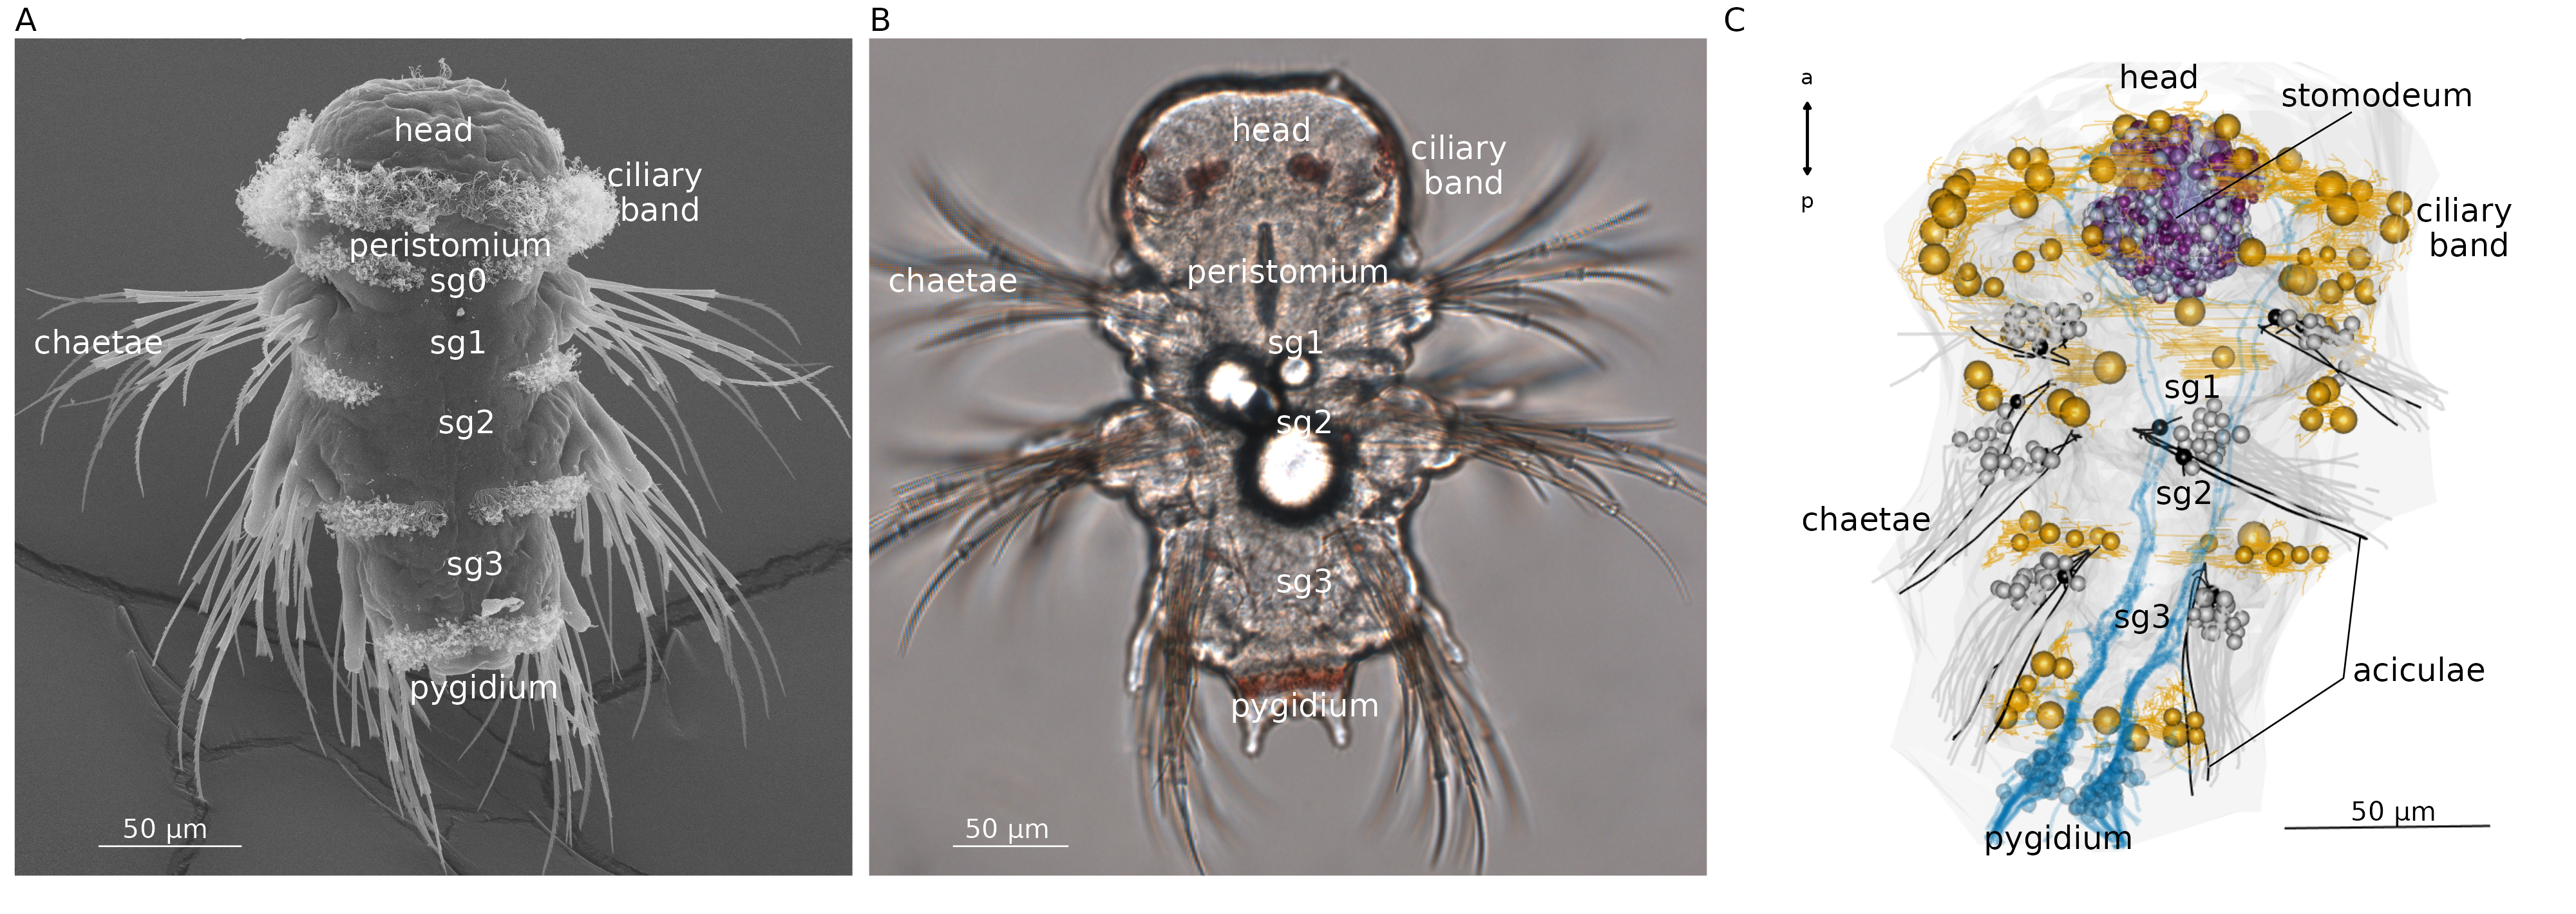
\includegraphics[width=1\textwidth,height=\textheight]{Figures/Figure1_fig_suppl1.png}

}

\caption{\textbf{Figure 1---figure supplement 1. Anatomy of the
three-day-old \emph{Platynereis dumerilii} larva.} (A) Scanning electron
micrograph of a three-day-old larva, ventral view. (B) Light microscopy
image of a three-day-old larva, ventral view. (C) Morphological
rendering of ciliary bands, stomodeum, aciculae, chaetae and pygidial
sensory neurons in the three-day-old larval volume.}

\end{figure}%

\begin{figure}[H]

{\centering \includegraphics[width=1\textwidth,height=\textheight]{Figures/Figure1_fig_suppl2.png}

}

\caption{\textbf{Figure 1---figure supplement 2. Morphological
parameters of neurons.} (A) Histogram of cable length for sensory,
inter- and motor neurons (twigs up to 2 microns were pruned). (B)
Histogram of cable length for fragments. (C) Histogram of the number of
postsynaptic sites for sensory, inter- and motor neurons. (D) Histogram
of the number of presynaptic sites for sensory, inter- and motor
neurons. (E) Relative difference of input and output synapses for
sensory, inter- and motor neurons. (F) Relationship of the number of
presynaptic sites and cable length for all neurons. Symbol size is
proportional to the number of postsynaptic sites. (G) Relationship of
the number of postsynaptic sites and cable length for all neurons.
Symbol size is proportional to the number of presynaptic sites. (H)
Relationship between cable length and the number of skeleton segments in
a neuron. Figure 1---figure supplement 1---source data 1. Source data
for all panels.}

\end{figure}%

\begin{figure}[H]

{\centering 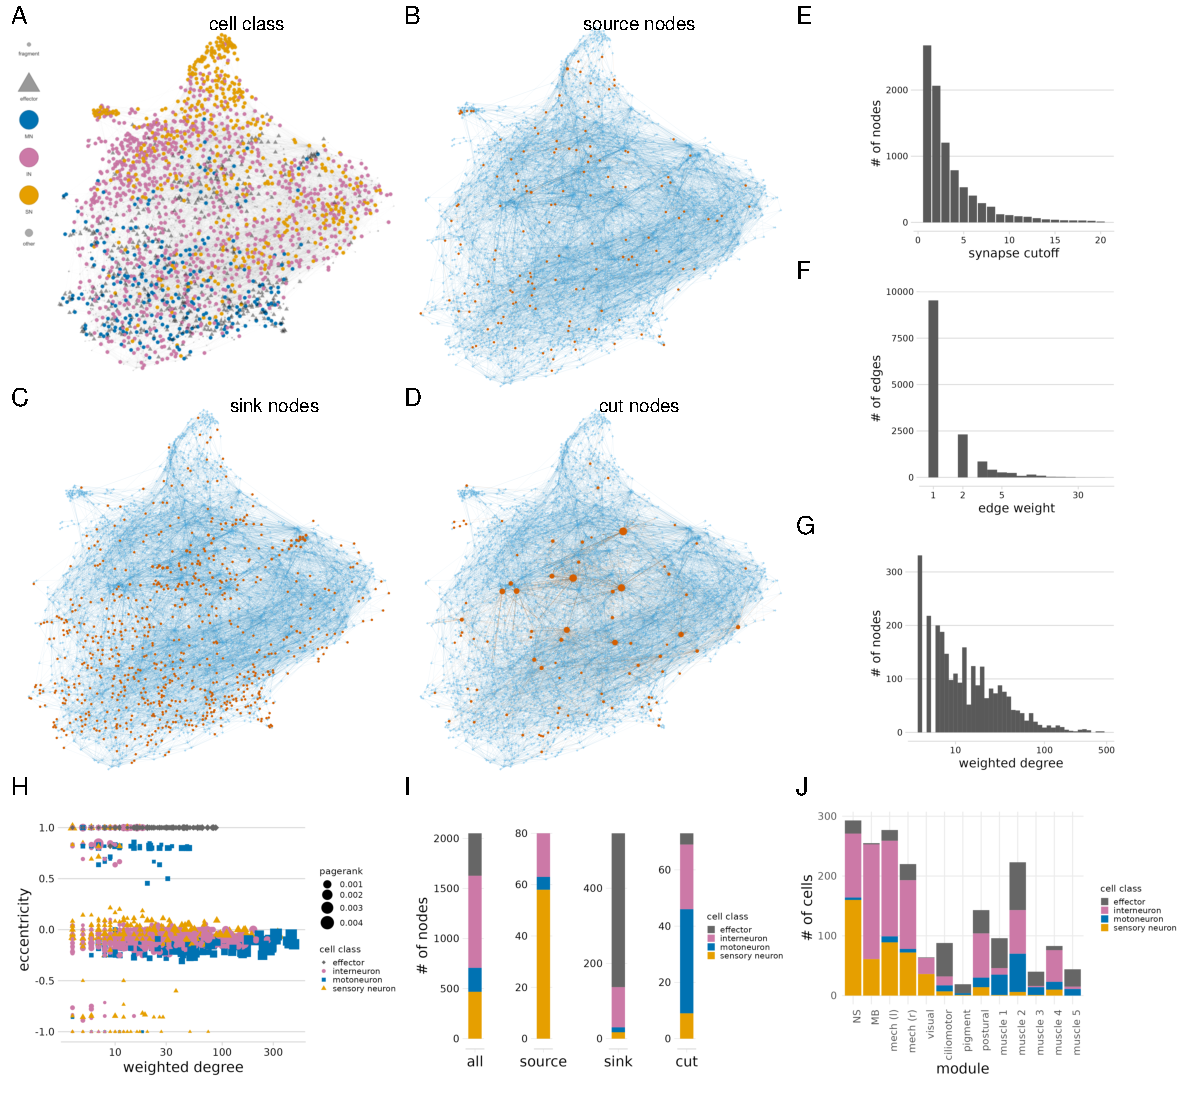
\includegraphics[width=1\textwidth,height=\textheight]{Figures/Figure2_fig_suppl1.png}

}

\caption{\textbf{Figure 2---figure supplement 1. Network parameters of
the connectome.} (A) The full connectome graph with nodes coloured by
cell class. (B) The full connectome graph with all source nodes coloured
in red. (C) The full connectome graph with all sink nodes coloured in
red. (D) The full connectome graph with all cut nodes coloured in red.
Node size is proportional to node weighted degree. (E) Number of nodes
in the largest network after deleting edges with an increasing number of
synapses from the connectome. (F) Distribution of edge weight (number of
synapses) in the connectome. (G) Distribution of node weighted degree in
the connectome. (G) Relationship of node eccentricity to node weighted
degree. (H) Number of sensory, inter-, motor neurons and effectors among
all nodes, or among source, sink and cut nodes. (I) Number of sensory,
inter-, motor neurons and effectors in the different modules of the
connectome. The source data file is the same as for Figure 2.}

\end{figure}%

\begin{figure}[H]

{\centering \includegraphics[width=1\textwidth,height=\textheight]{Figures/Figure2_fig_suppl2.png}

}

\caption{\textbf{Figure 2---figure supplement 2. Connectivity of
connectome modules.} (A) Grouped connectivity matrix of the 13
connectome modules. (B) Sankey information-flow network of the 13
connectome modules (coloured as in Figure 2). Left-to-righ connections
are indicated with solid grey lines, right-to-left connections with
dashed magenta lines. Only connections with \textgreater20 synapses are
shown. Line width is proportional to the square root of synapse number.
(C) Number of Leiden modules detected in the full connectome graph as a
function of the resolution parameter. Figure 2---figure supplement
2---source data 1. The source data matrix as csv file.}

\end{figure}%

\begin{figure}[H]

{\centering \includegraphics[width=1\textwidth,height=\textheight]{Figures/Figure2_fig_suppl3.png}

}

\caption{\textbf{Figure 2---figure supplement 3. Neuropils formed by
connectome modules.} (A) Neuropils of the visual, anterior NS, MB and
central brain and postural control modules. (B) VNC neurite tracks of
the left and right mechanosensory, the postural control and the MB and
central brain modules.}

\end{figure}%

\begin{figure}[H]

{\centering 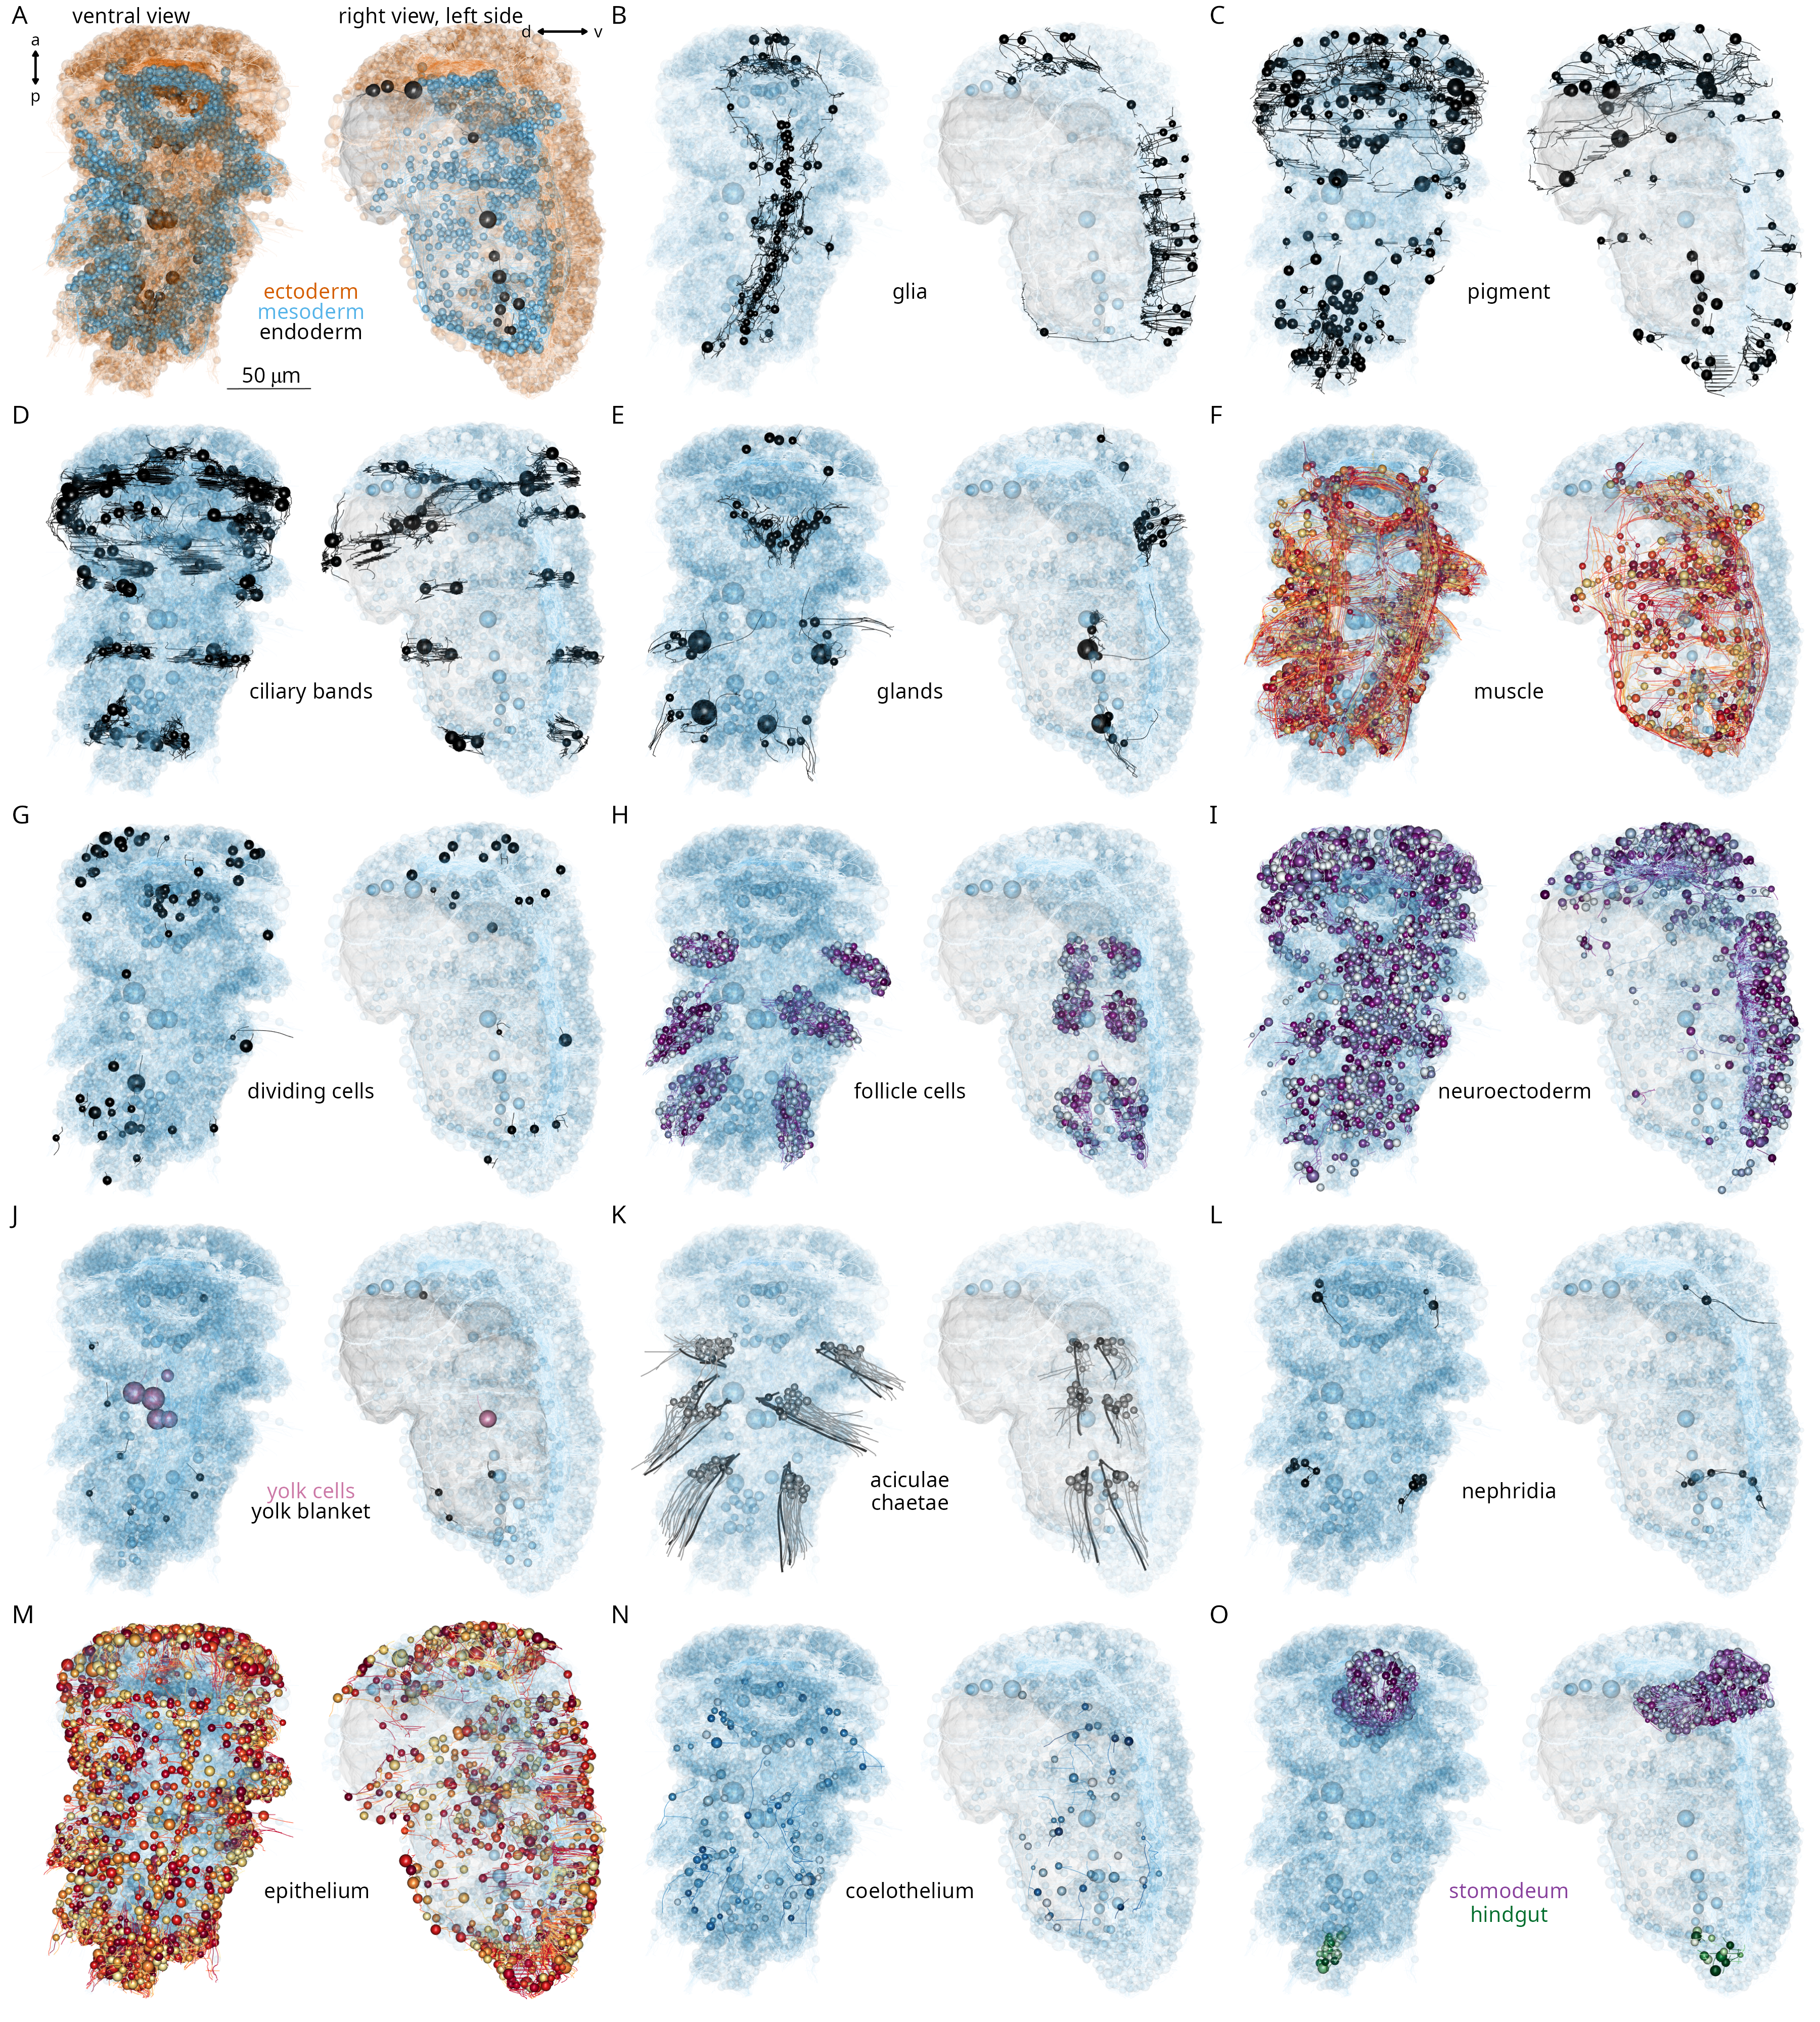
\includegraphics[width=1\textwidth,height=\textheight]{Figures/Figure3_fig_suppl1.png}

}

\caption{\textbf{Figure 3---figure supplement 1. Major cell classes in
the three-day-old \emph{Platynereis} larva.} Morphological rendering of
(A) all cells coloured by germ layer, (B) glia cells, (C) pigment cells,
(D) ciliary band cells, (E) gland cells, (F) muscle cells, (G) dividing
cells, (H) acicular and chaetal follicle cells, (I) developing cells of
the neuroectoderm, (J) yolk and yolk blanket cells (K) aciculoblasts and
chaetoblasts, (L) proto- and metanephridia, (M) epithelial cells, (N)
coelothelial cells and (O) cells of the stomodeum and hindgut. In all
panels all other cells of the body are shown in transparent cyan and the
yolk in grey for reference. Each panel shows a ventral (left) and a left
view (right). Left views only show cells on the left body side.}

\end{figure}%

\begin{figure}[H]

{\centering \includegraphics[width=1\textwidth,height=\textheight]{Figures/Figure3_fig_suppl2.png}

}

\caption{\textbf{Figure 3---figure supplement 2. Major annotations of
cell types.} All neuronal cell types and their major annotations,
including germ layer, body segment, cell class, morphological features
and transmitter phenotypes. Columns were arranged based on the
hierarchical clustering of annotations by the ward.D2 method. Figure
3---figure supplement 2---source data 1. The annotation matrix in txt
format with cell-types ordered by their celltype annotation
(celltype1-celltype202).}

\end{figure}%

\begin{figure}[H]

{\centering \includegraphics[width=1\textwidth,height=\textheight]{Figures/Figure3_fig_suppl3.png}

}

\caption{\textbf{Figure 3---figure supplement 3. Number of skeletons for
double annotations. } Number of skeletons annotated with two annotations
across the volume. This also includes cells outside the connectome
(e.g.~some interneurons with low connectivity). Figure 3---figure
supplement 3---source data 1. The data in tibble format.}

\end{figure}%

\begin{figure}[H]

{\centering \includegraphics[width=1\textwidth,height=\textheight]{Figures/Figure3_fig_suppl4.png}

}

\caption{\textbf{Figure 3---figure supplement 4. Example neuronal cell
types. } Morphological rendering of example neuronal cell types in (A)
anterior and (B) ventral view.}

\end{figure}%

\begin{figure}[H]

{\centering \includegraphics[width=1\textwidth,height=\textheight]{Figures/Figure3_fig_suppl5.png}

}

\caption{\textbf{Figure 3---figure supplement 5. Average Sholl diagrams
for all symmetrical neuronal cell types.} Sholl diagrams were plotted
for the left (top) and right (bottom) body sides Figure 3---figure
supplement 5---source data 1. Source data of left and right Sholl
plots.}

\end{figure}%

\begin{figure}[H]

{\centering 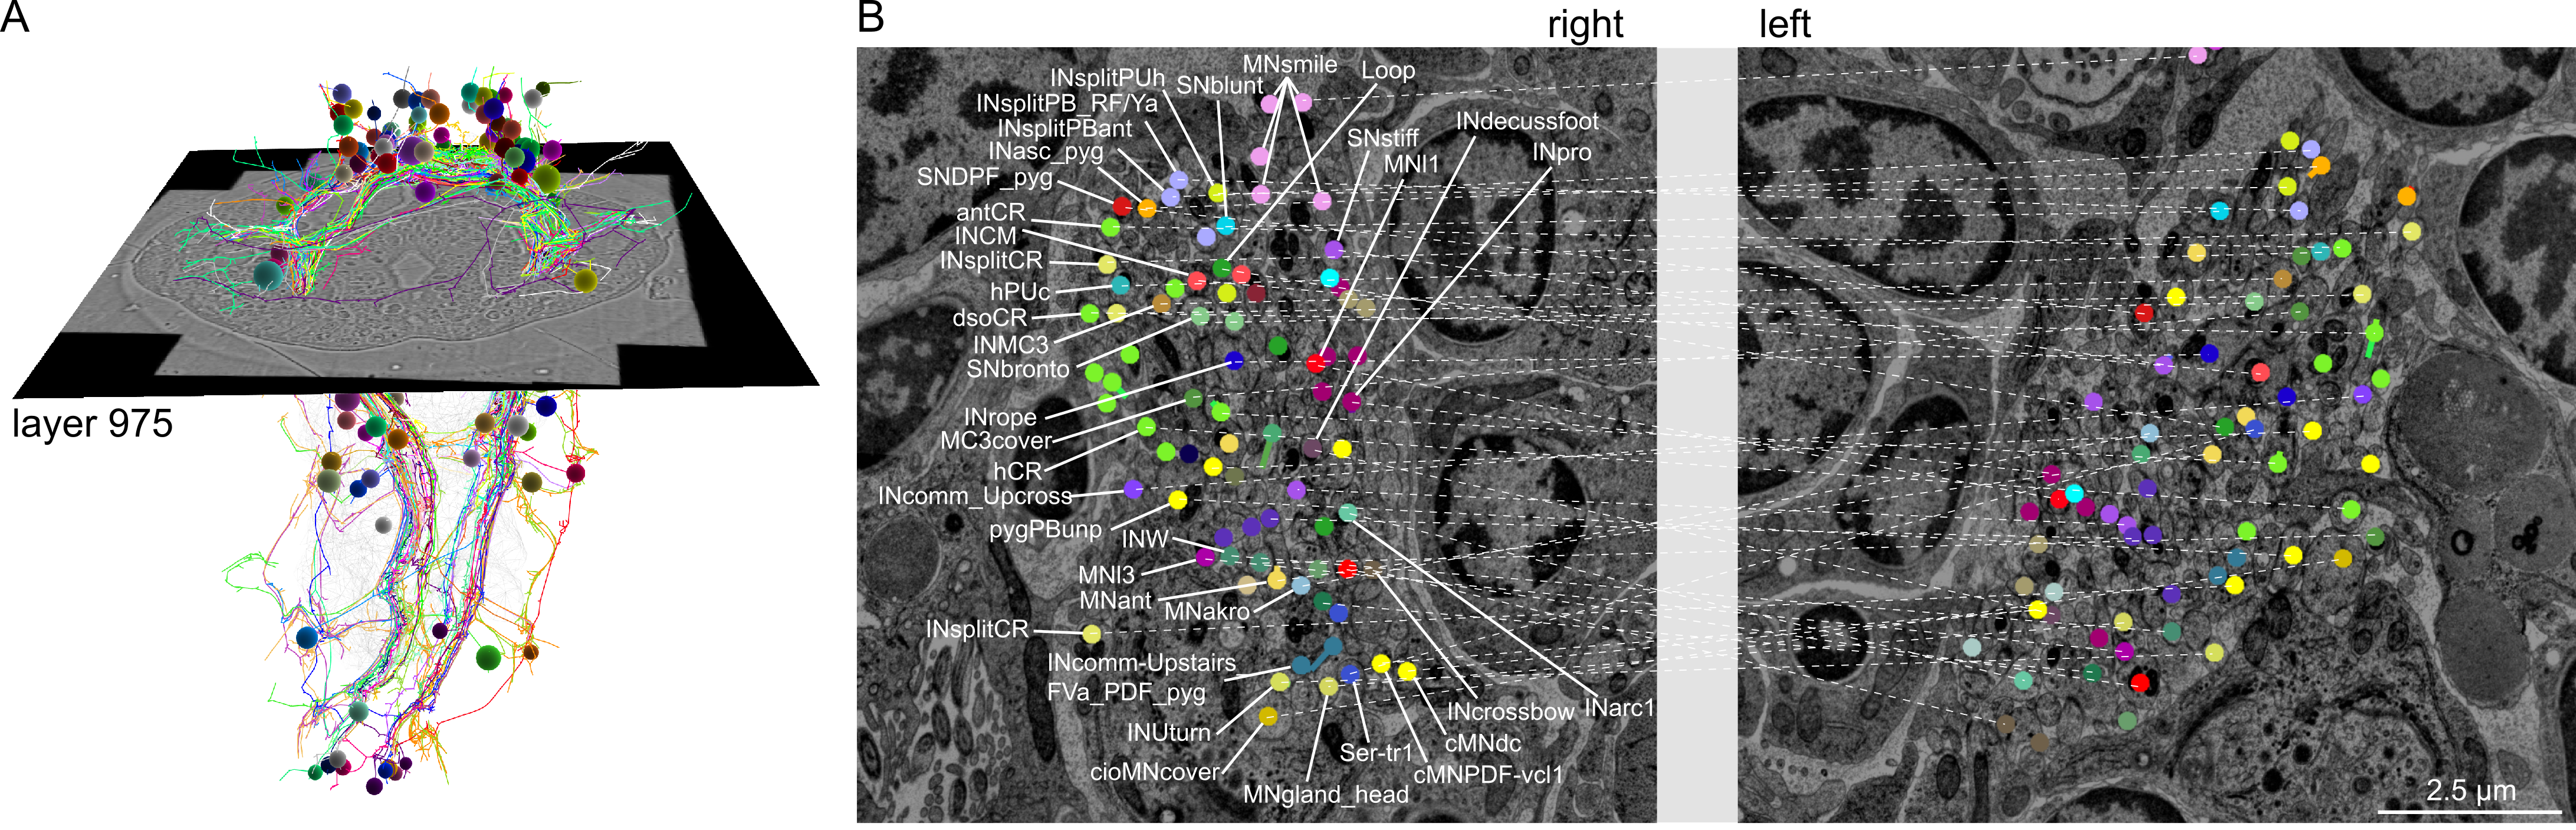
\includegraphics[width=1\textwidth,height=\textheight]{Figures/Figure3_fig_suppl6.png}

}

\caption{\textbf{Figure 3---figure supplement 6. Position of axons of
left-right symmetric cell pairs. } Position of bilaterally symmetrical
cell types on the right and left side of the stomodeum. Left-right pairs
from the same cell type are connected by a thin line. Left panel shows
the position of the layer (later 975) in the volume.}

\end{figure}%

\begin{figure}[H]

{\centering 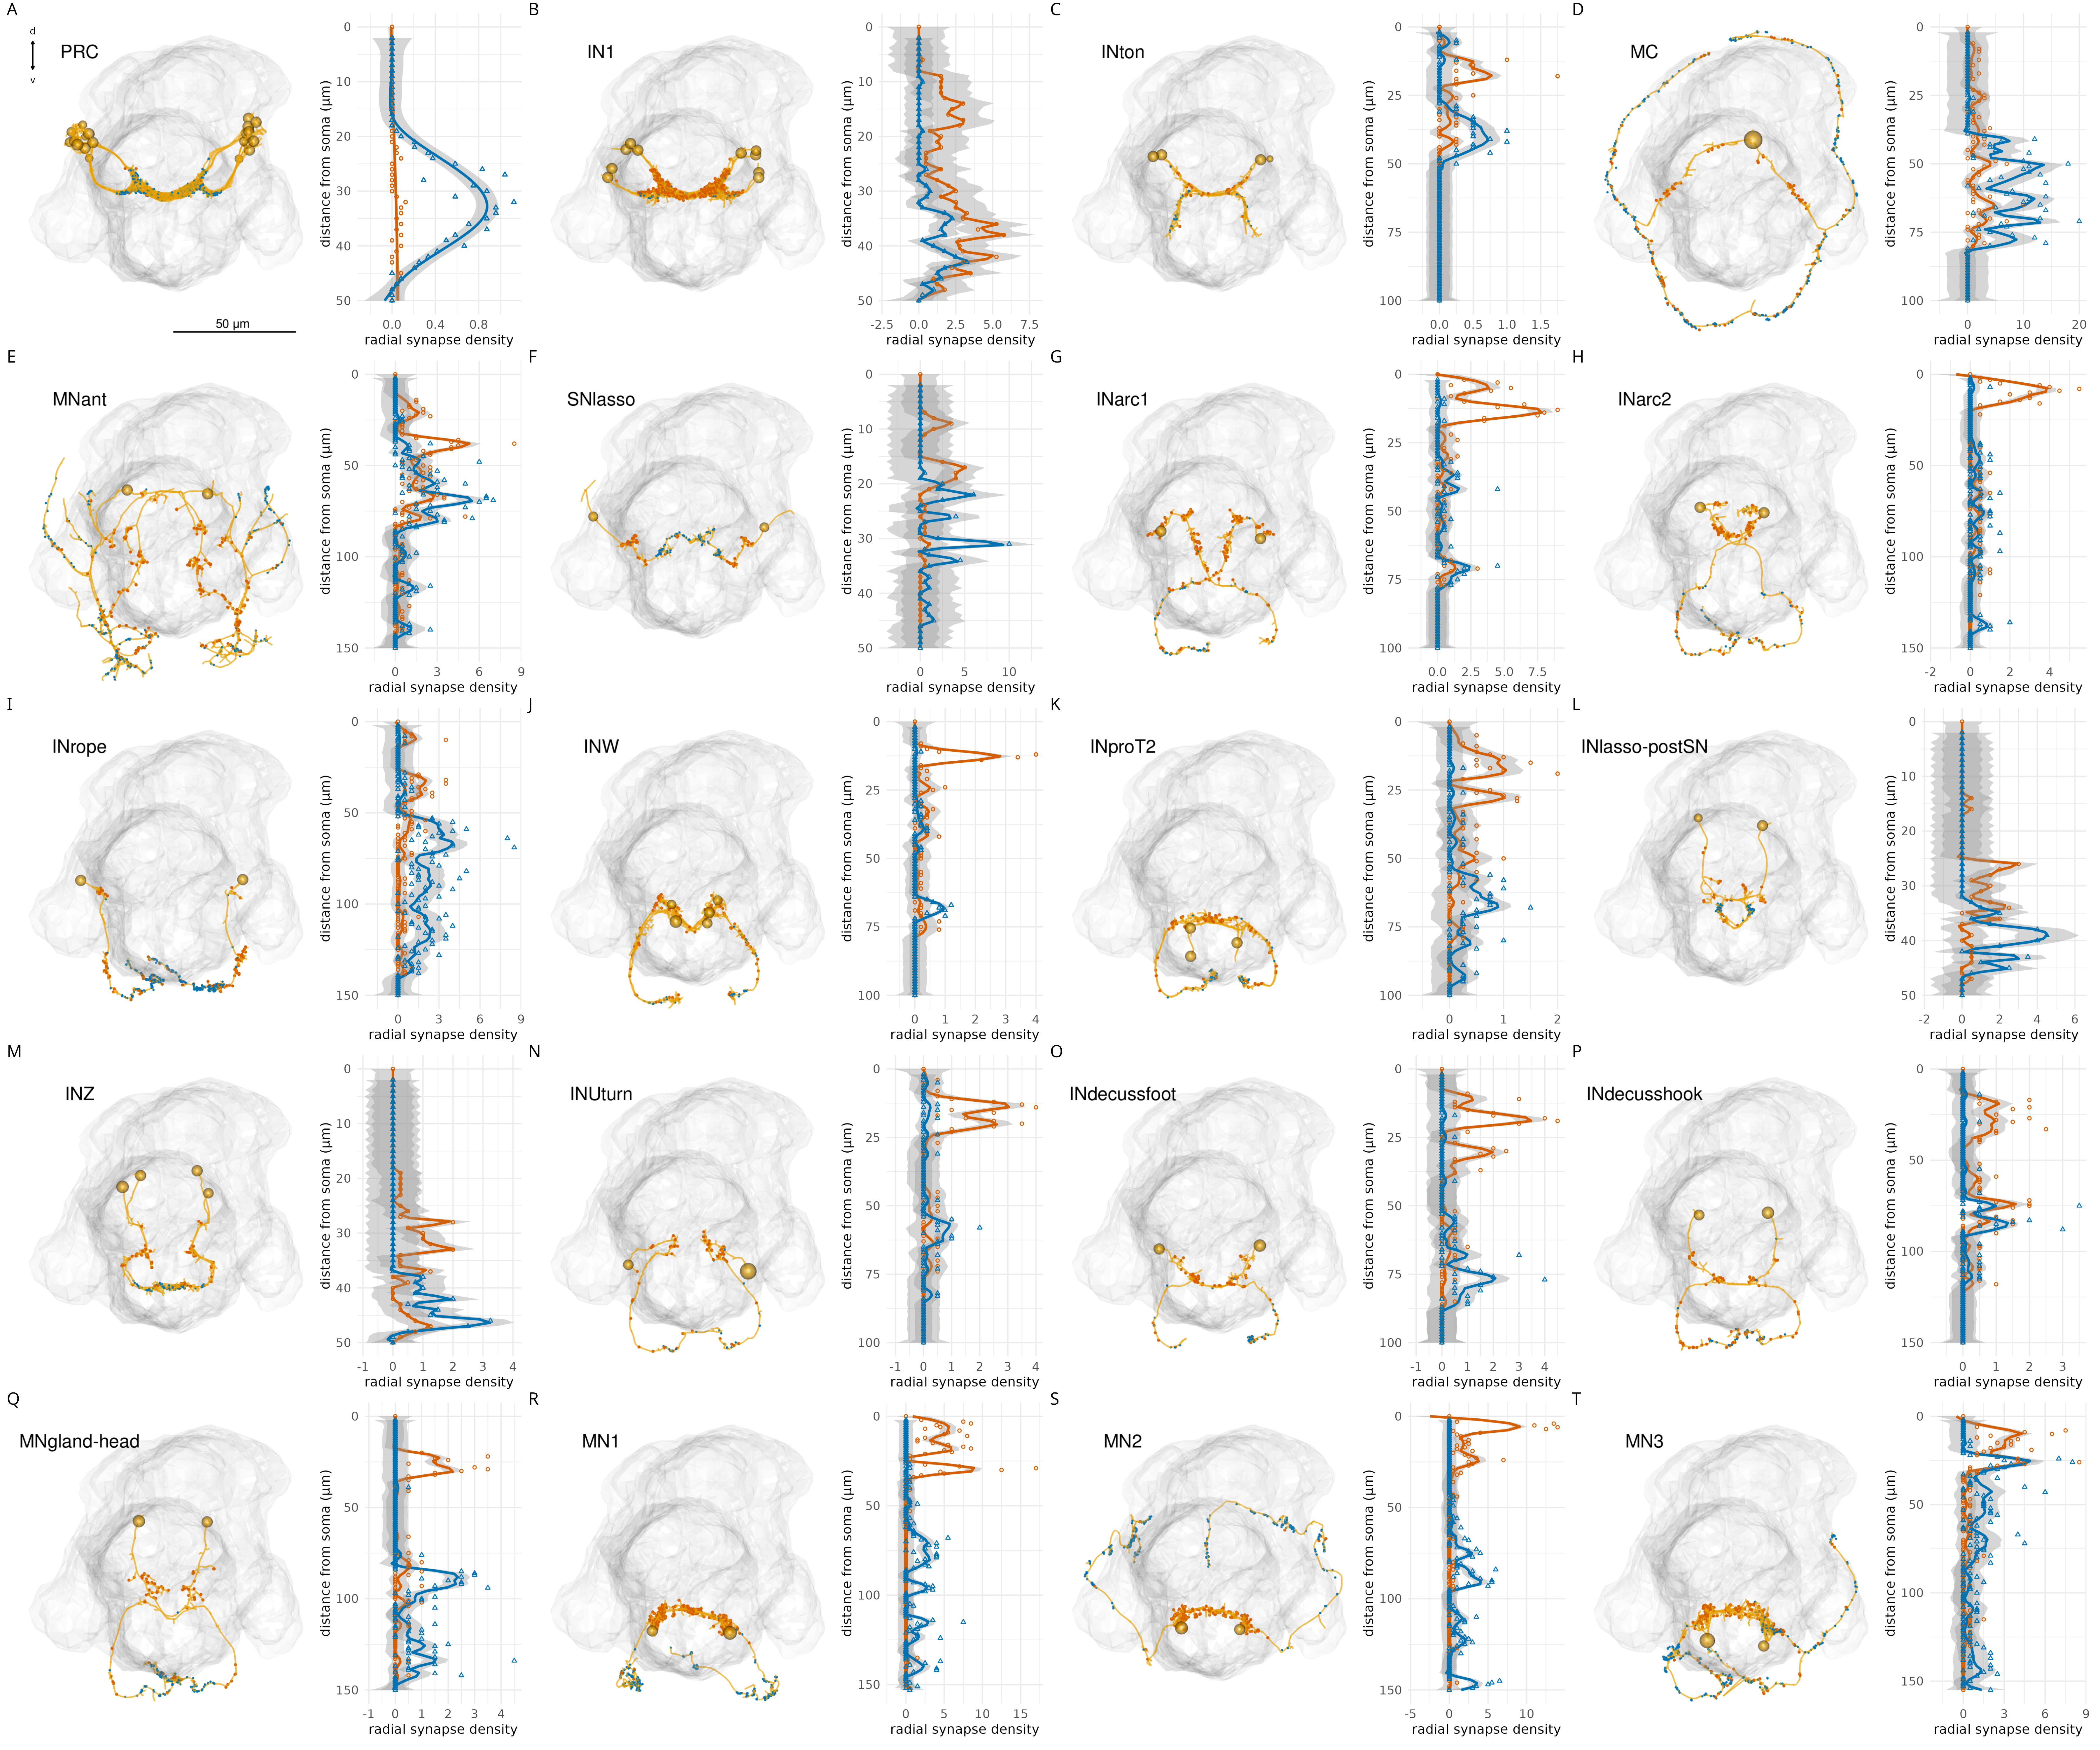
\includegraphics[width=1\textwidth,height=\textheight]{Figures/Figure3_fig_suppl7.png}

}

\caption{\textbf{Figure 3---figure supplement 7. Radial density of
incoming and outgoing synapses in head neurons. } (A-T) Morphological
renderings of selected head cell types with input and output synapses
(left panels) and radial density plots of incoming and outgoing synapses
(right panels). Synapse density was calculated from the root node (soma)
and was averaged for different neurons of the same cell type.
Figure3---figure supplement 7---source data 1. Radial density data of
incoming and outgoing synapses for all 202 cell types.}

\end{figure}%

\begin{figure}[H]

{\centering 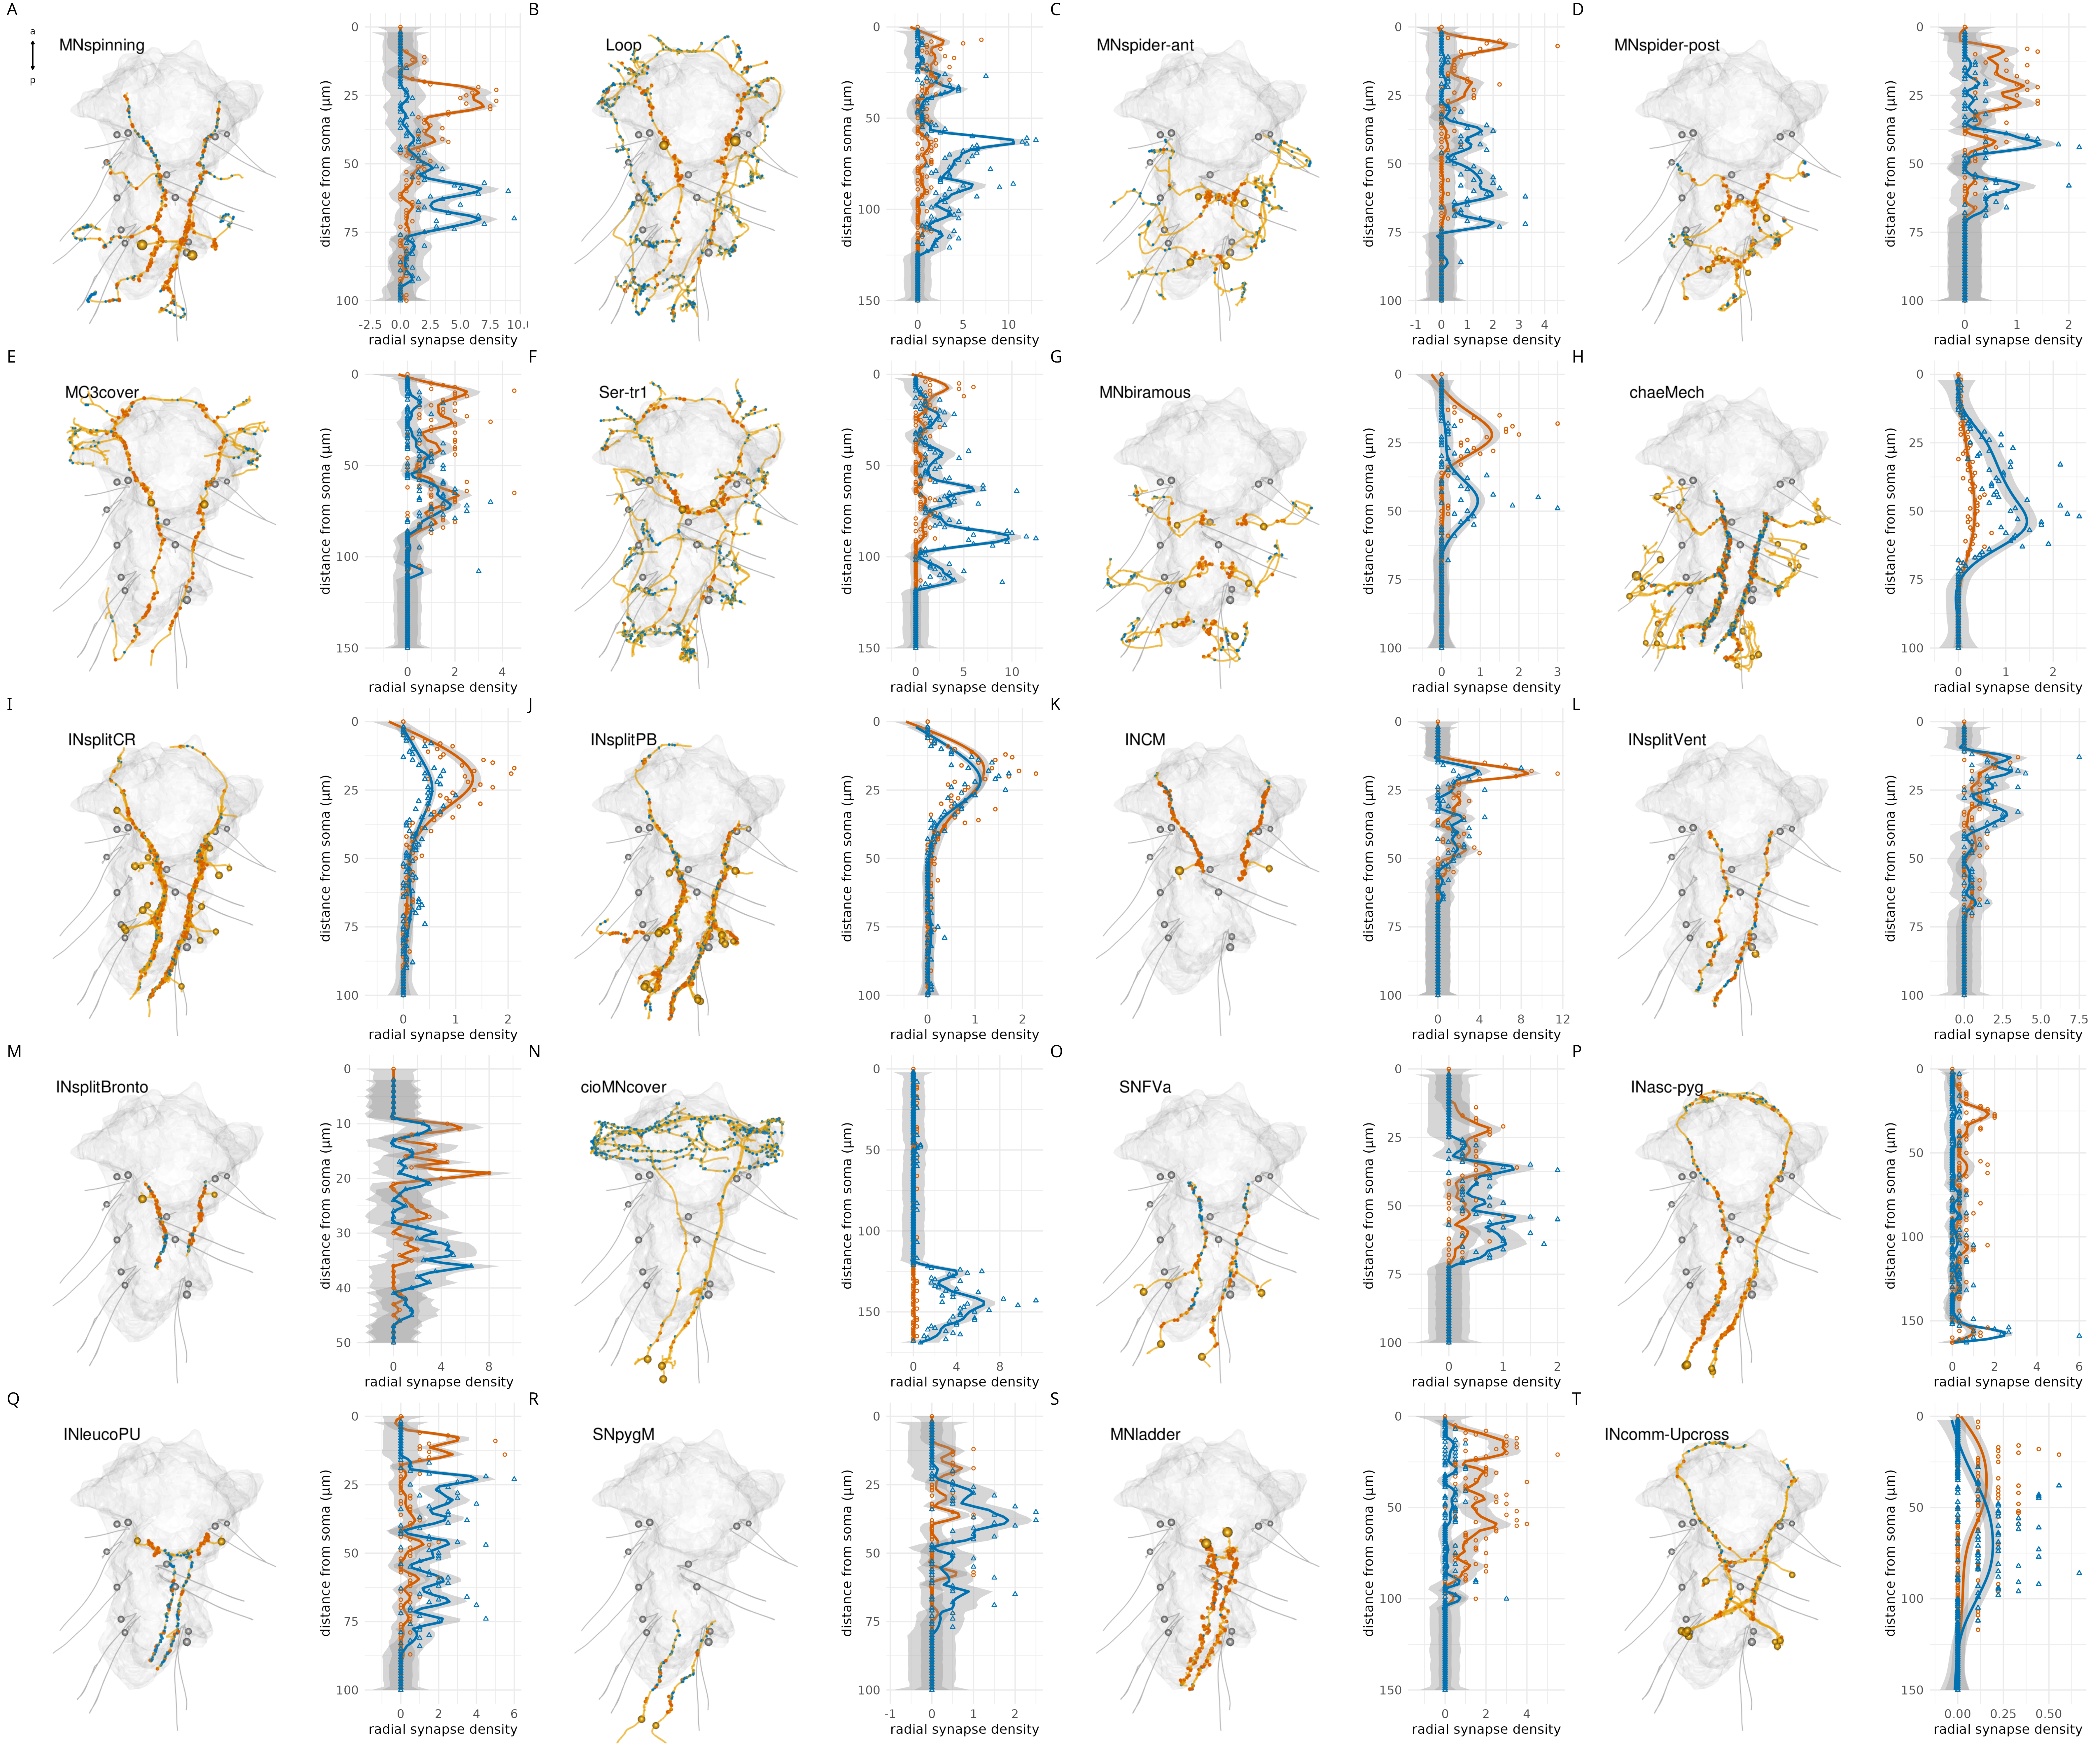
\includegraphics[width=1\textwidth,height=\textheight]{Figures/Figure3_fig_suppl8.png}

}

\caption{\textbf{Figure 3---figure supplement 8. Radial density of
incoming and outgoing synapses in trunk neurons. } (A-T) Morphological
renderings of selected trunk cell types with input and output synapses
(left panels) and radial density plots of incoming and outgoing synapses
(right panels). Synapse density was calculated from the root node (soma)
and was averaged for different neurons of the same cell type. Source
data are the same as for Figure3---figure supplement 7.}

\end{figure}%

\begin{figure}[H]

{\centering \includegraphics[width=1\textwidth,height=\textheight]{Figures/Figure4_fig_suppl1.png}

}

\caption{\textbf{Figure 4---figure supplement 1. The \emph{Platynereis}
larval connectome grouped by cell type. } Matrix representation of the
cell-type connectome. Source data are the same as for Figure 4.}

\end{figure}%

\begin{figure}[H]

{\centering \includegraphics[width=0.8\textwidth,height=\textheight]{Figures/Figure4_fig_suppl2.png}

}

\caption{\textbf{Figure 4---figure supplement 2. Comparison of
connectivity between the left and right body sides.} (A) Grouped
synaptic connectivity matrix of all cell types. The neuronal cell types
1-202 are shown separately for cells on the left or right body side
(defined by soma position). The postsynaptic groups represent all
neuronal cell types 1-202 and non-neuronal cell types 1-91. For the
postsynaptic groups, both body sides were included. Values in each row
have been divided by the number of cells in the corresponding
presynaptic group to obtain the average number of presynapses per cell
in that group. For display only, values are shown as the square root of
synapse number. Figure 4---figure supplement 2---source data 1. Source
data for left-right cell-type connectivity in tibble format.}

\end{figure}%

\begin{figure}[H]

{\centering \includegraphics[width=1\textwidth,height=\textheight]{Figures/Figure4_fig_suppl3.png}

}

\caption{\textbf{Figure 4---figure supplement 3. Comparison of
connectivity between the left and right body sides.} Correlation matrix
of the postsynaptic connectivity of neuronal cell types subdivided by
body side. Values represent the row-by-row Pearson's correlation
coefficients of the synaptic connectivity table in Figure 4---figure
supplement 2 calculated for left and right members of each cell type.
Figure 4---figure supplement 3---source data 1. Source data for the
Pearson correlatelation data for the left-right cell-type comparisons.}

\end{figure}%

\begin{figure}[H]

{\centering 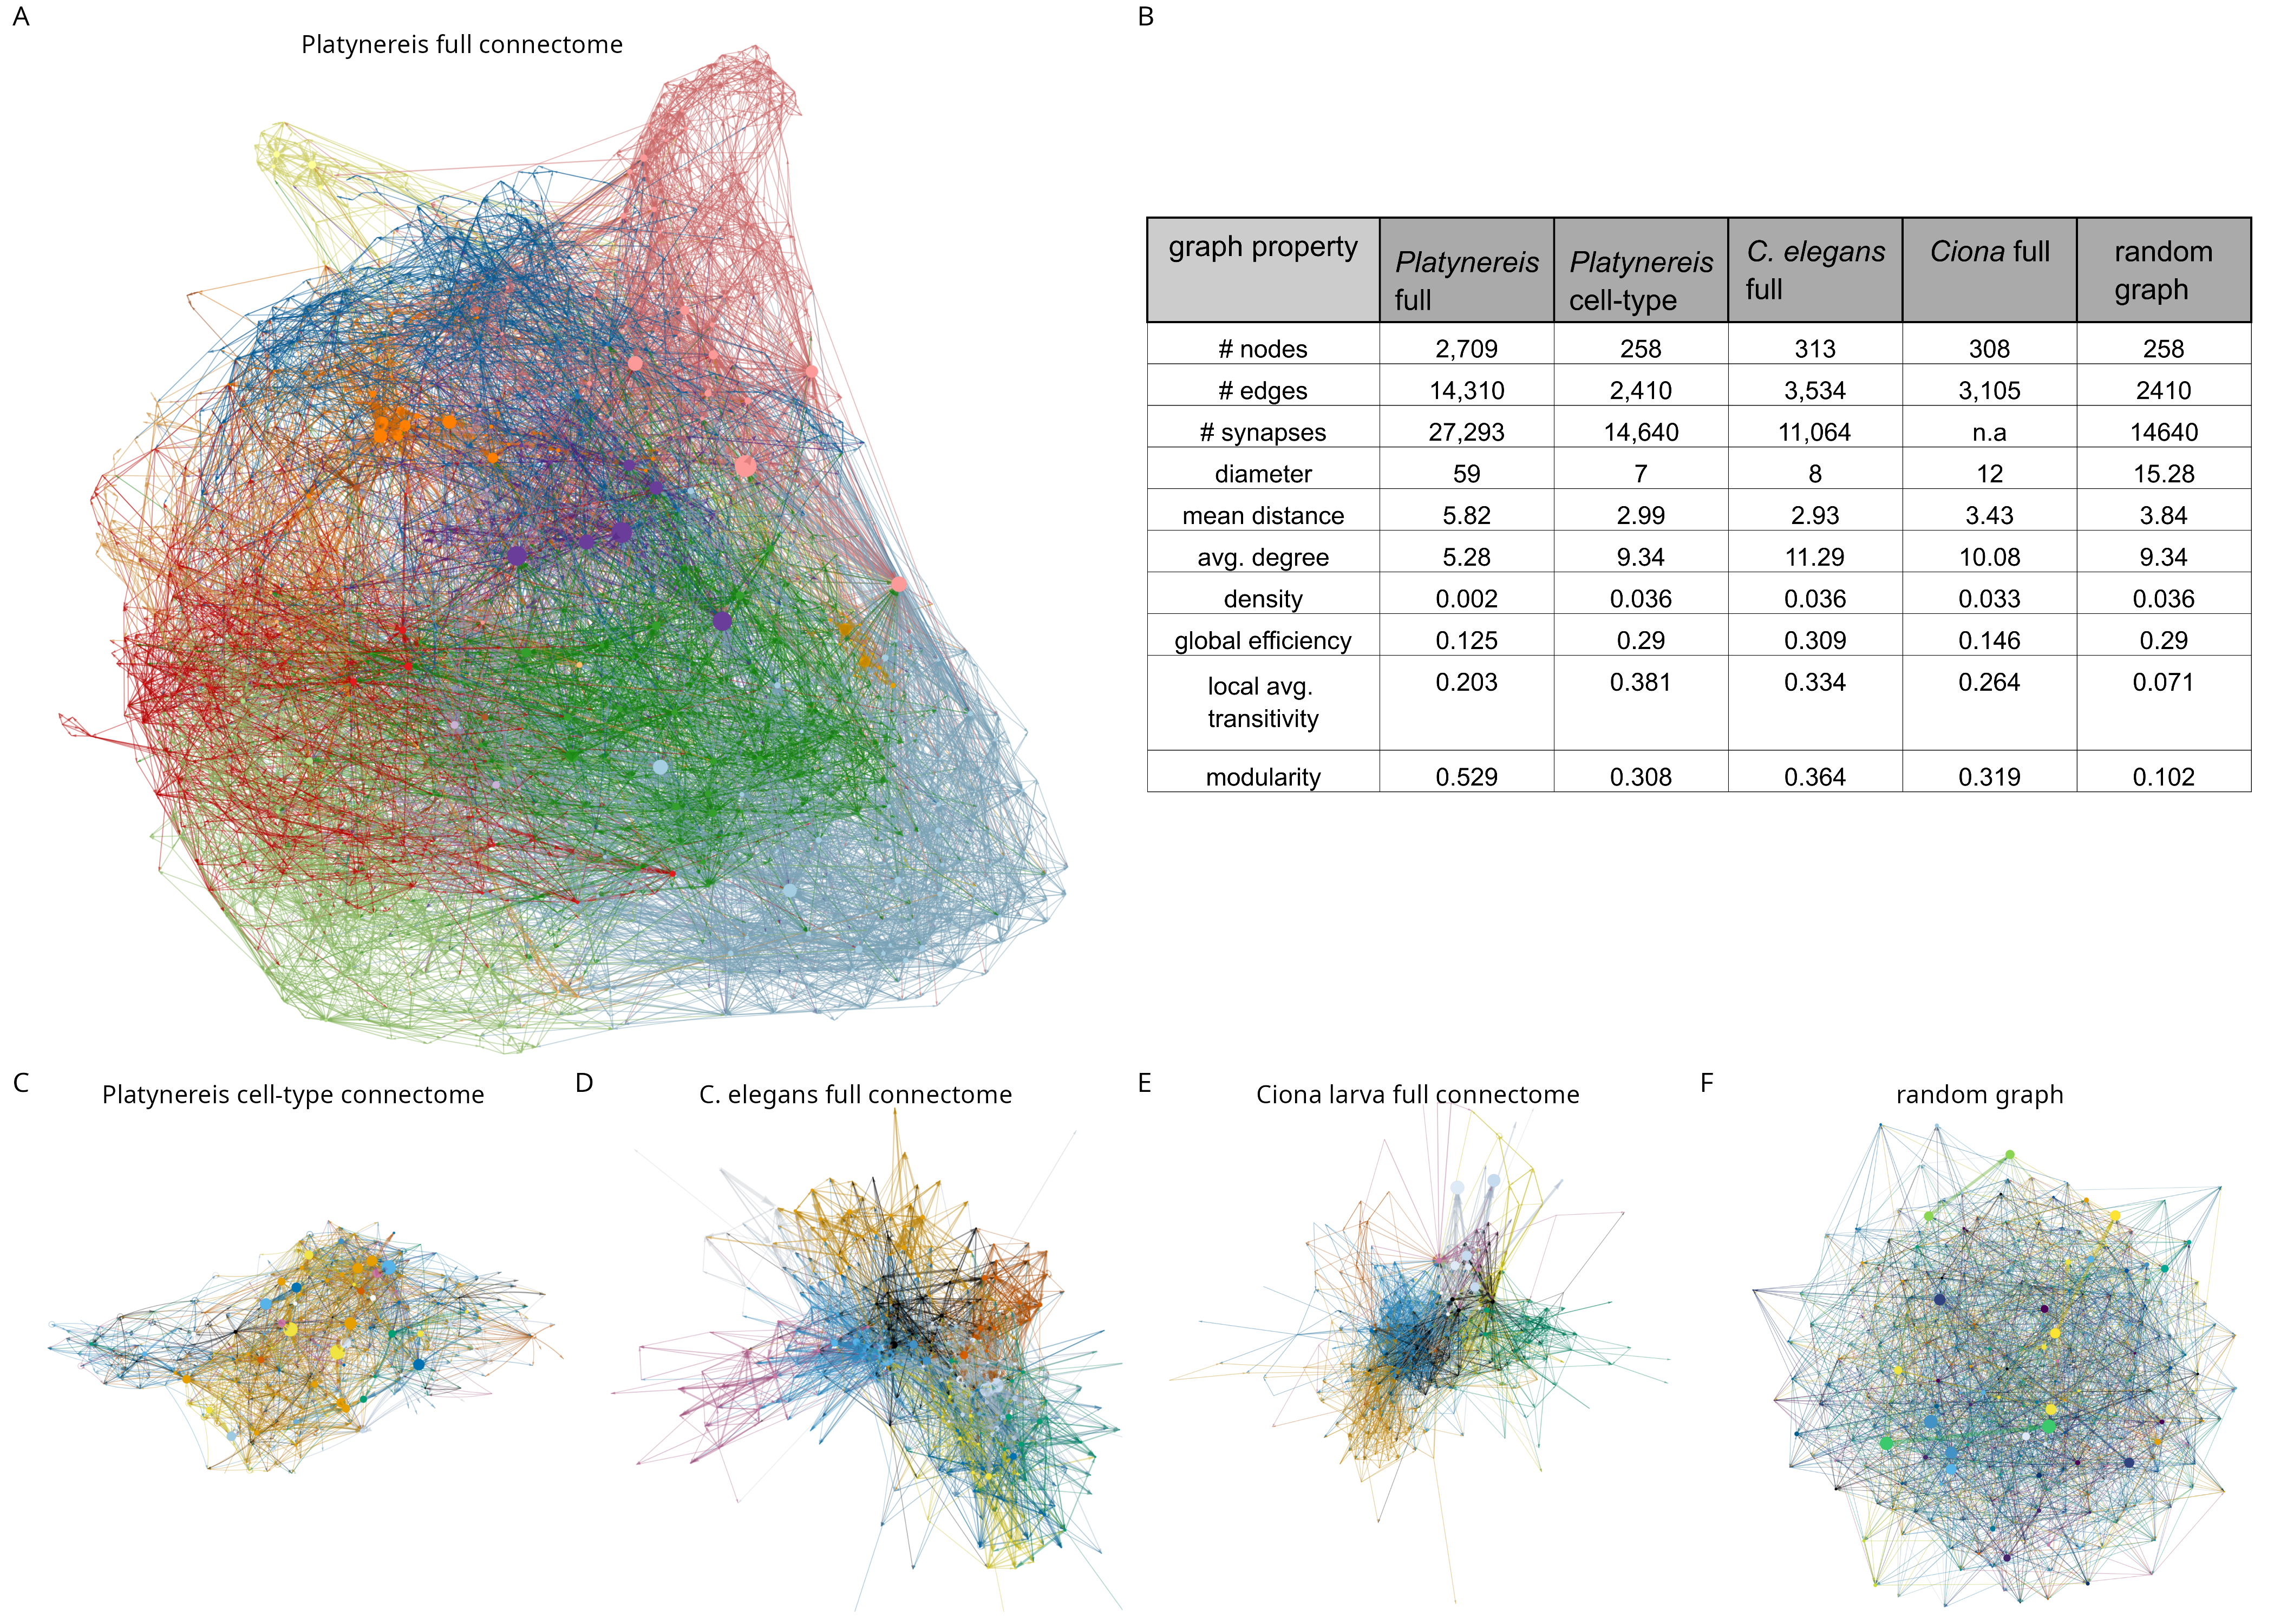
\includegraphics[width=1\textwidth,height=\textheight]{Figures/Figure4_fig_suppl4.png}

}

\caption{\textbf{Figure 4---figure supplement 4. Network properties of
the \emph{Platynereis}, \emph{C. elegans} and \emph{Ciona} connectomes
in comparison to a random graph } (A) Network graph of the full
\emph{Platynereis} connectome, coloured by Leiden modules. (B) Summary
table of network statistics for the four connectome networks and mean
values for 100 Erdős-Rényi random graphs with the same number of nodes
and edges as the \emph{Platynereis} cell-type graph. (C) The
\emph{Platynereis} grouped cell-type-level connectome coloured by Leiden
modules. (D) The \emph{C. elegans} connectome (excluding the pharynx
network) coloured by Leiden module. (E) The \emph{Ciona} larval
connectome coloured by Leiden module. (F) An Erdős-Rényi random graph
coloured by Leiden module.}

\end{figure}%

\begin{figure}[H]

{\centering 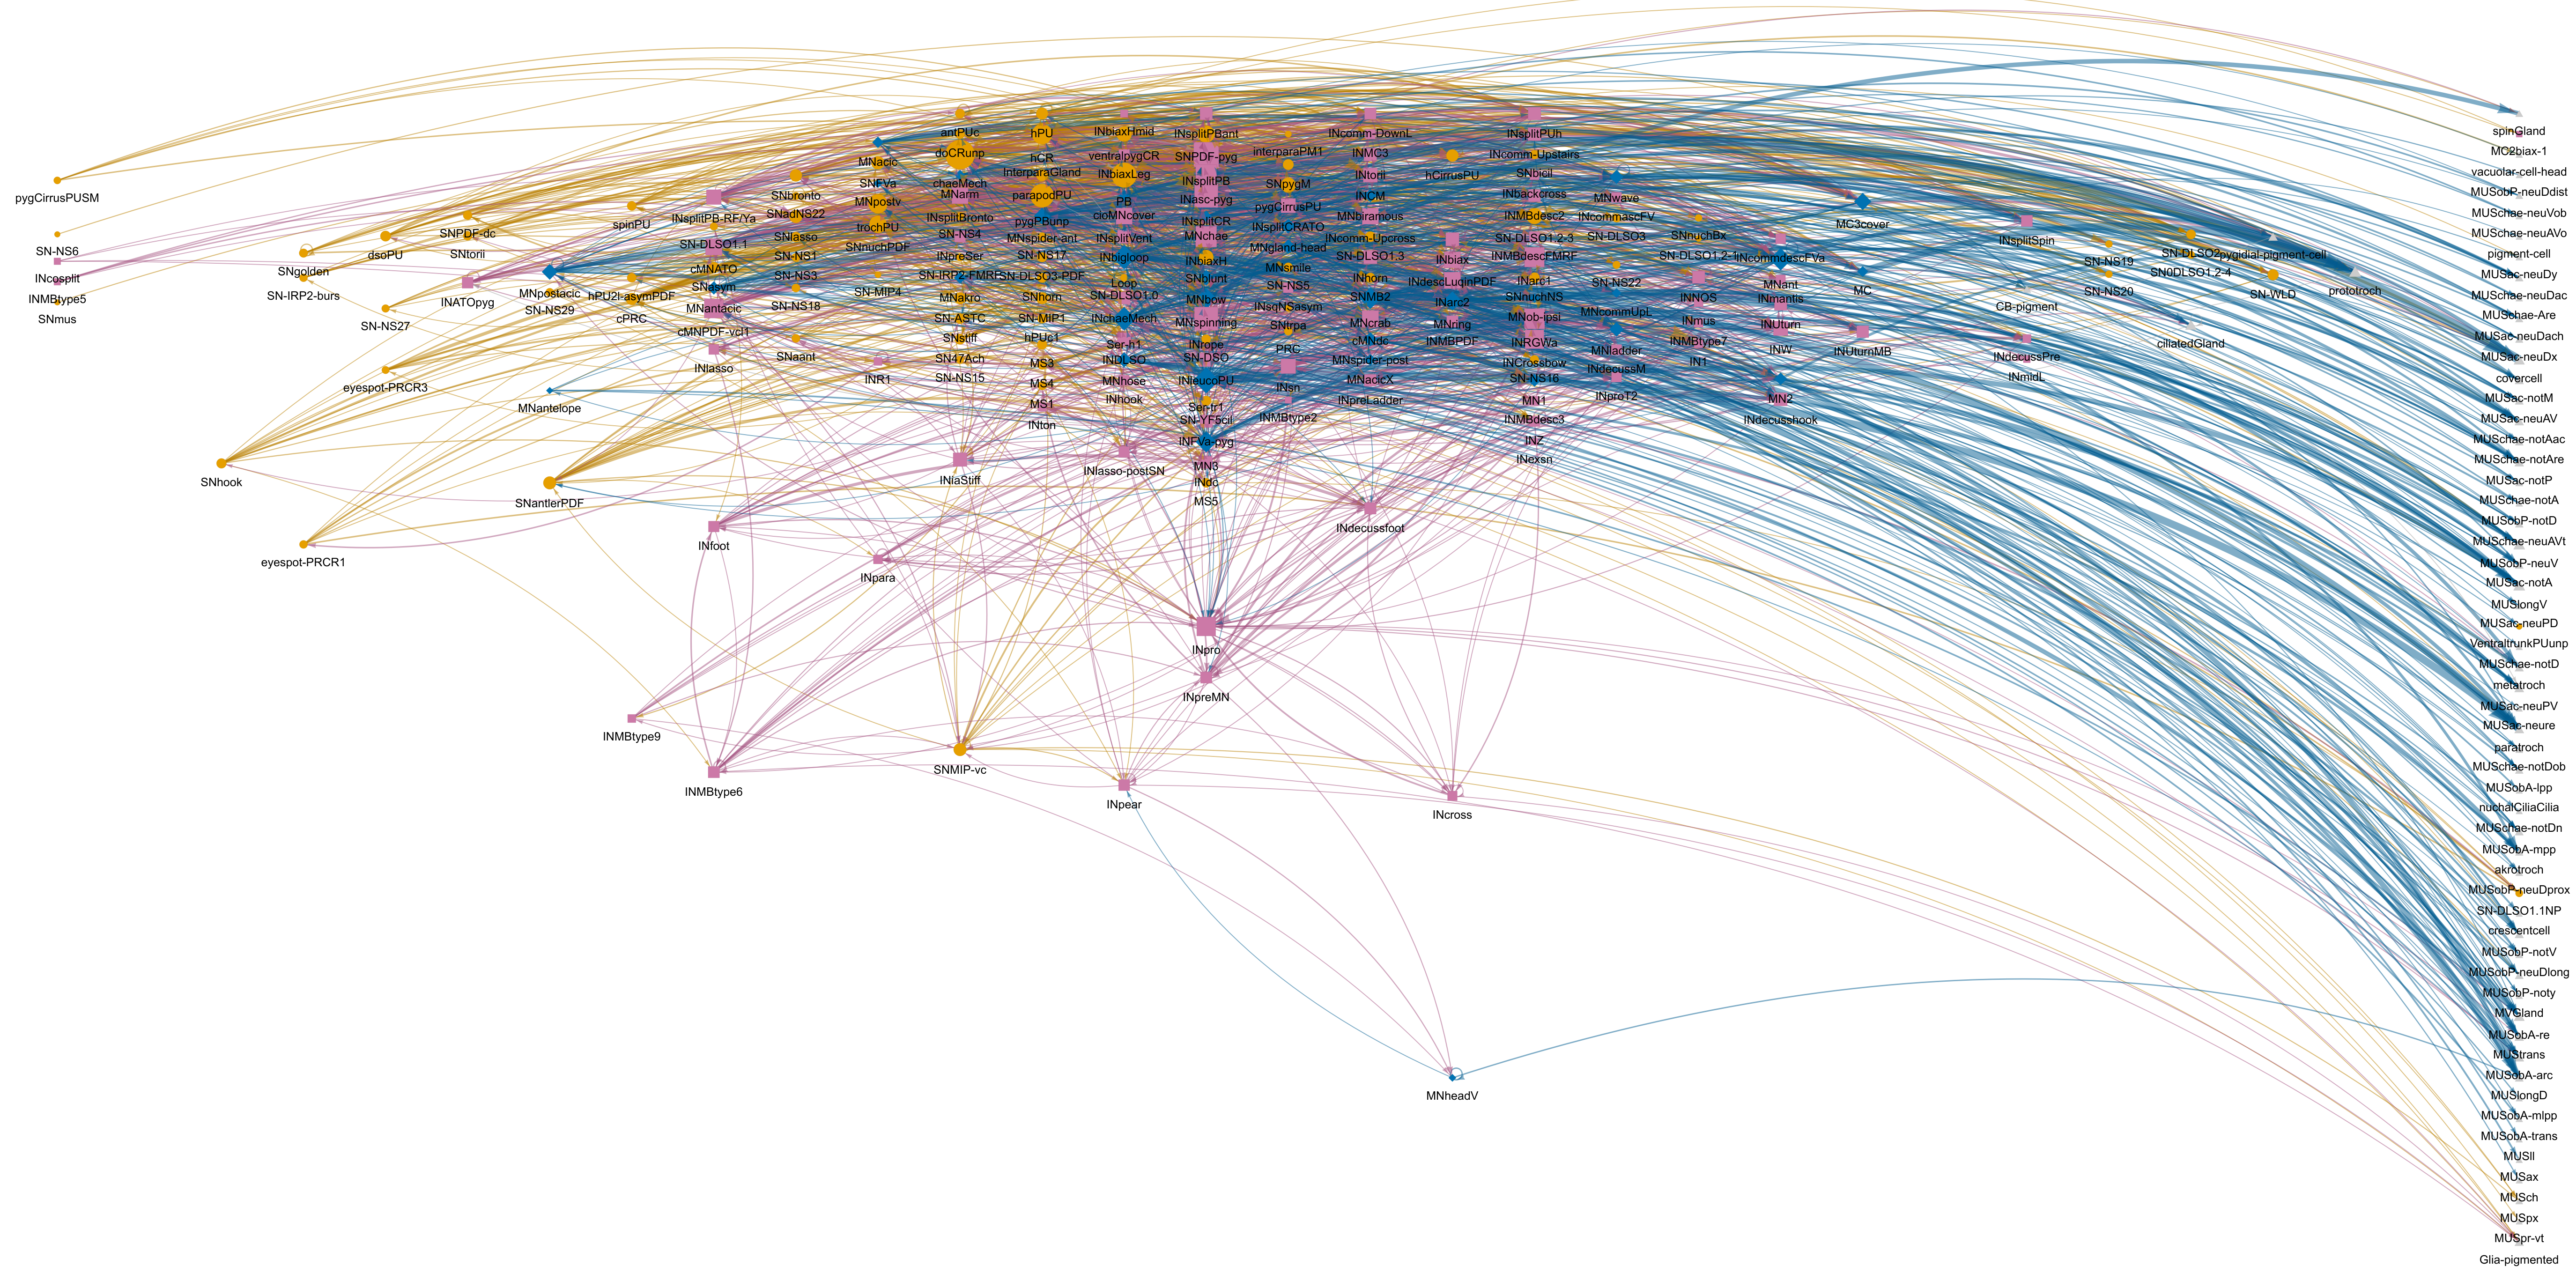
\includegraphics[width=1\textwidth,height=\textheight]{Figures/Figure4_fig_suppl5.png}

}

\caption{\textbf{Figure 4---figure supplement 5. Sensory neurons
categorised by path length to effectors.}}

\end{figure}%

\begin{figure}[H]

{\centering 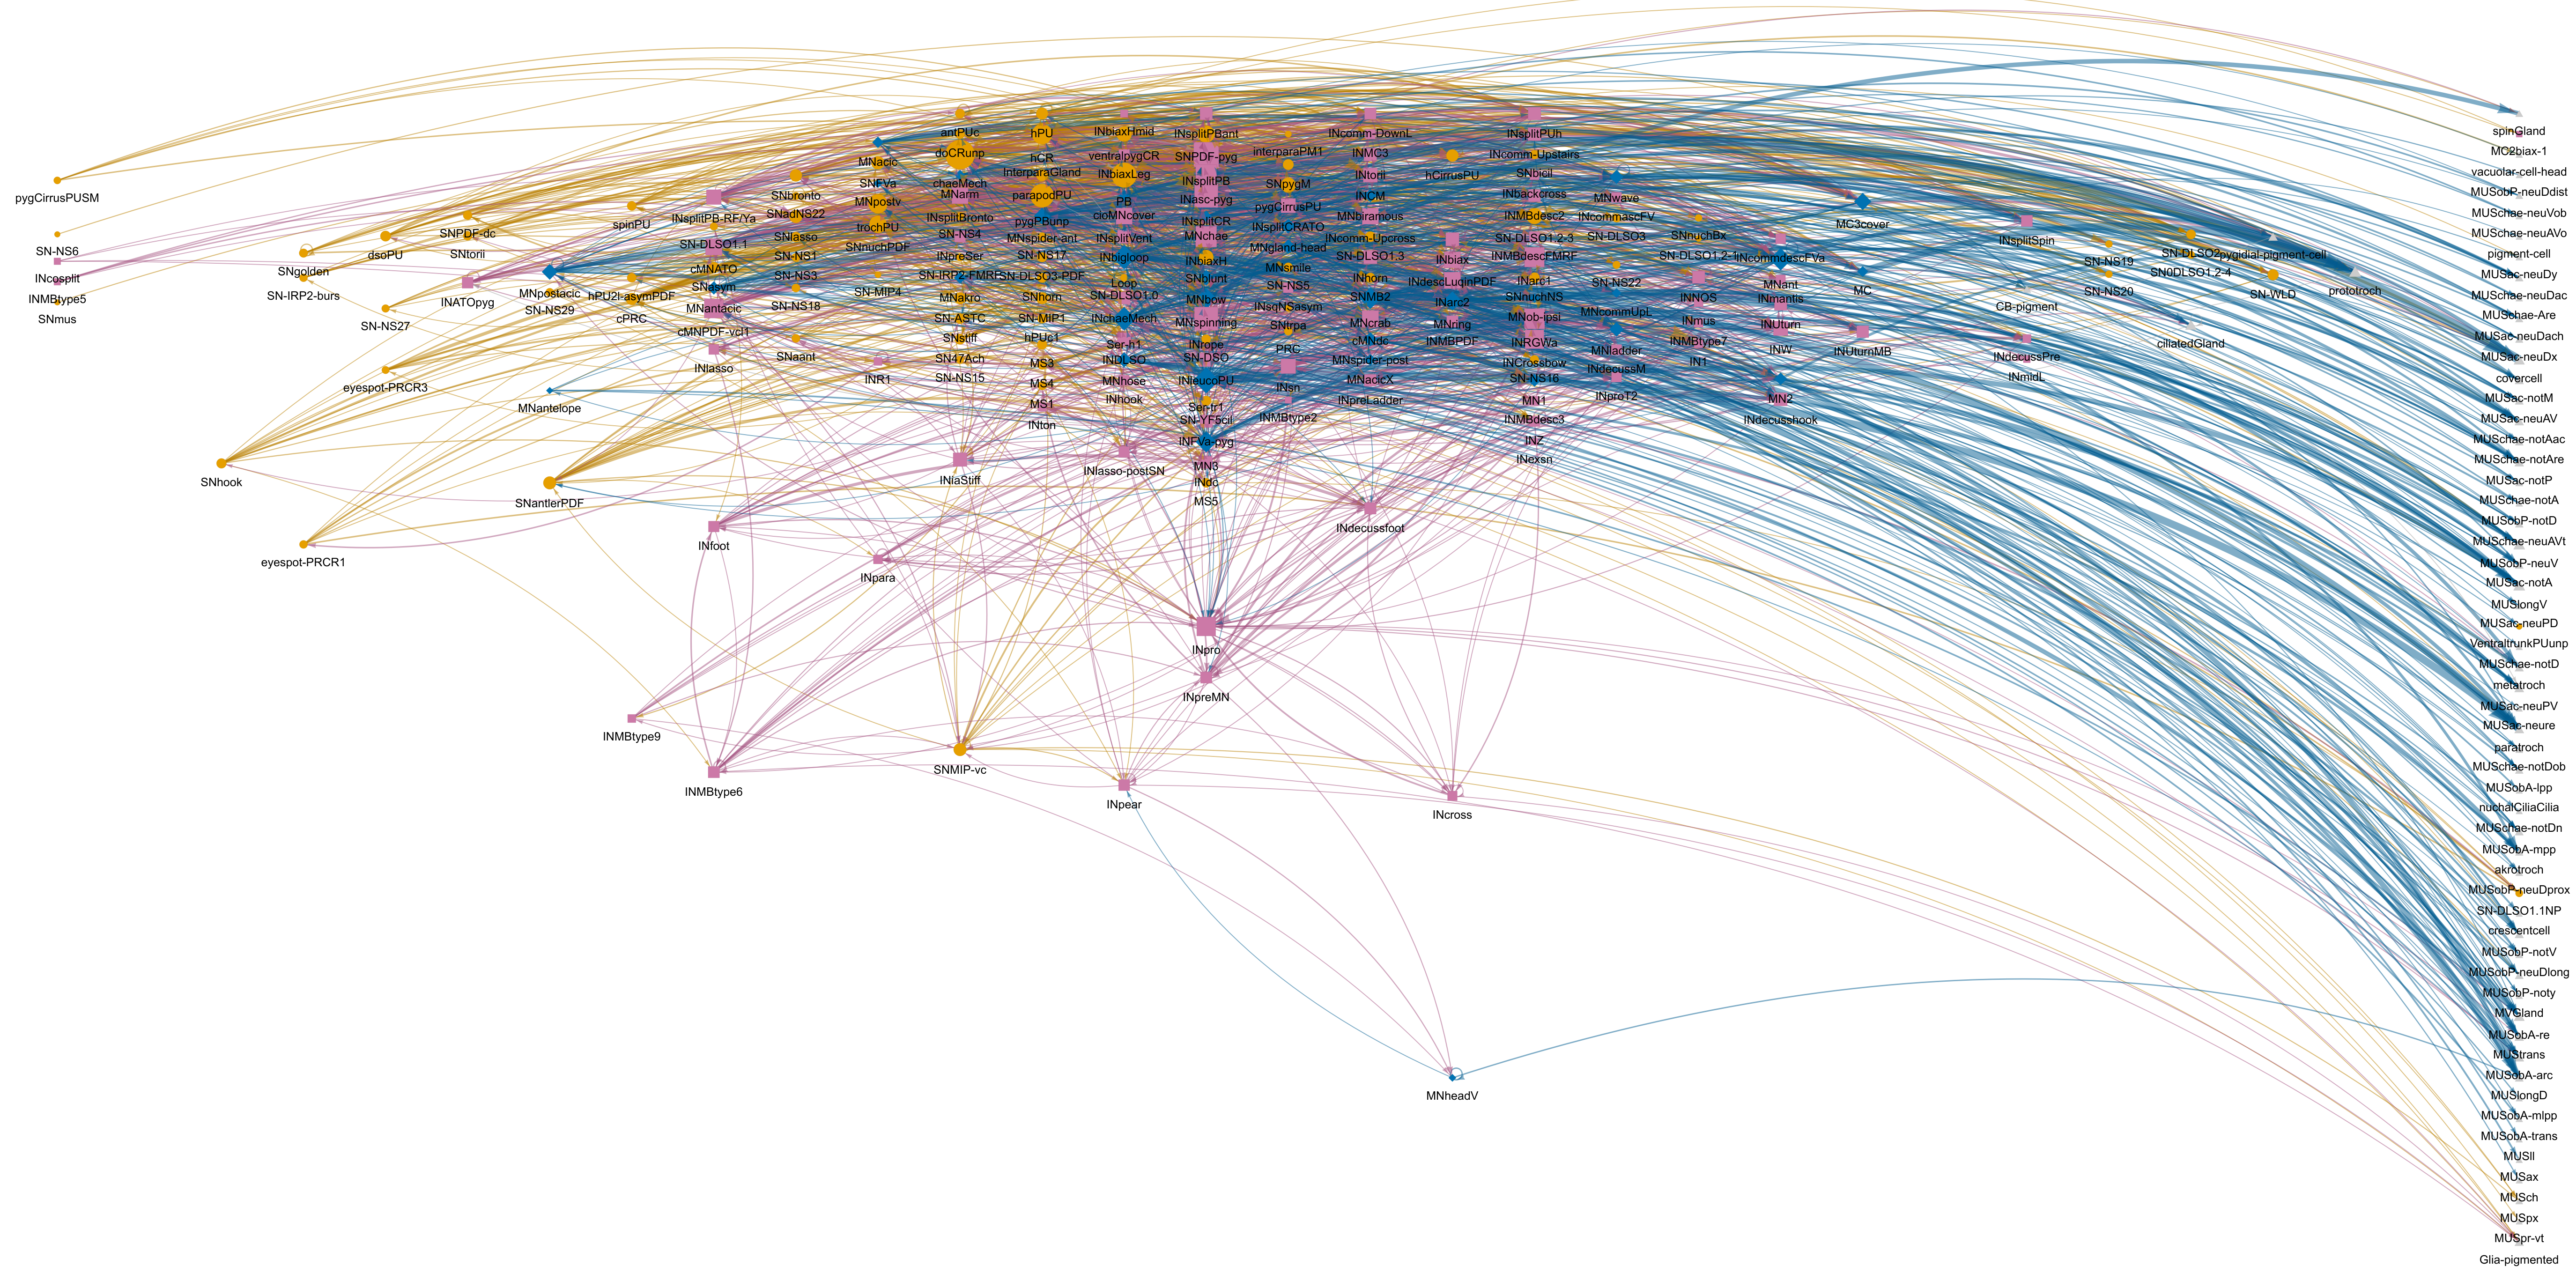
\includegraphics[width=1\textwidth,height=\textheight]{Figures/Figure4_fig_suppl6.png}

}

\caption{\textbf{Figure 4---figure supplement 6. Grouped connectivity
graph. } Cell-type level connectome graph with node horizontal positions
proportional to the relative ratio of incoming (postsynaptic) and
outgoing (presynpatic) sites. Cell-type names are shown under the nodes.
Figure 4---figure supplement 6---source data 1. The network in
visNetwork format saved as an R RDS source file, saved with bz2
compression. Can be loaded with read\_rds().}

\end{figure}%

\begin{figure}[H]

{\centering \includegraphics[width=1\textwidth,height=\textheight]{Figures/Figure5_fig_suppl1.png}

}

\caption{\textbf{Figure 5---figure supplement 1. Neurons with dense
cored vesicles.} (A, B) Morphological rendering of neurons with dense
cored vesicles, ventral (A) and anterior (B) views.}

\end{figure}%

\begin{figure}[H]

{\centering 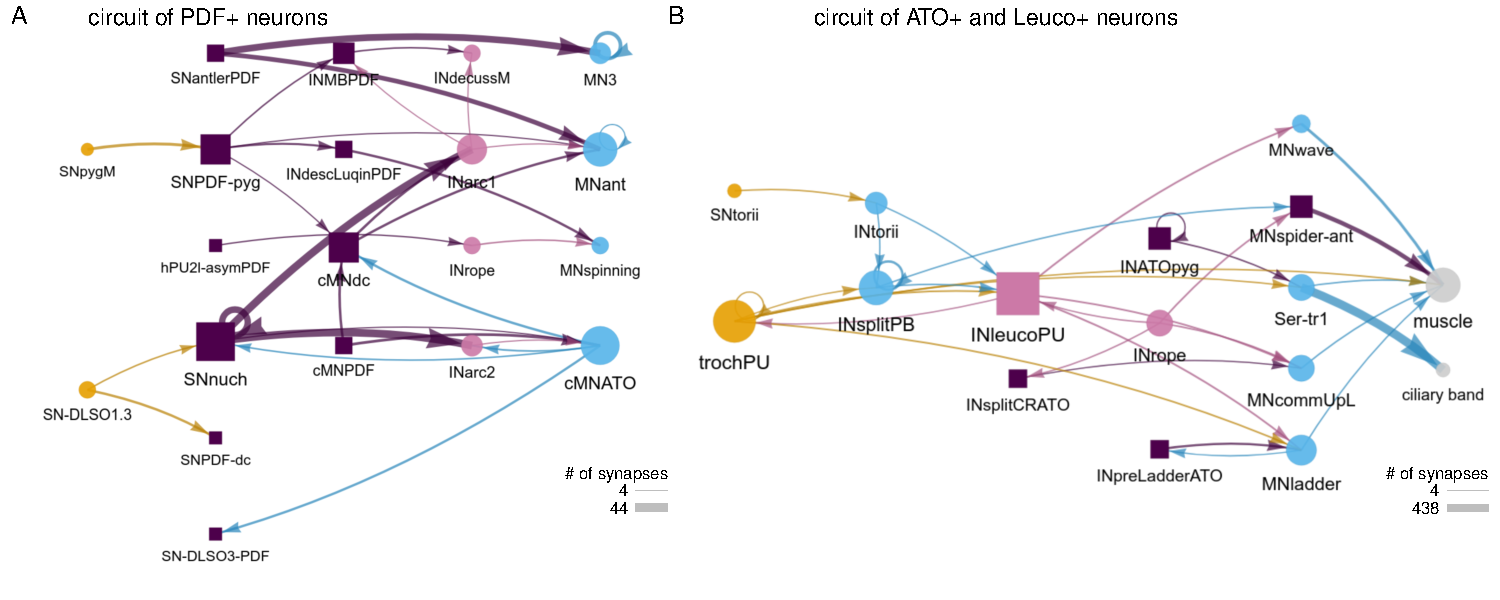
\includegraphics[width=1\textwidth,height=\textheight]{Figures/Figure5_fig_suppl2.png}

}

\caption{\textbf{Figure 5---figure supplement 2. Circuits of PDF,
allatotropin/orexin and leucokinin neurons. } (A) Network diagram of
PDF-expressing neurons and their pre- and postsynaptic partners (B)
Network diagram of allatotropin/orexin- and leucokinin-expressing
neurons and their pre- and postsynaptic partners.
Neuropeptide-expressing cell types are represented with squares.}

\end{figure}%

\begin{figure}[H]

{\centering 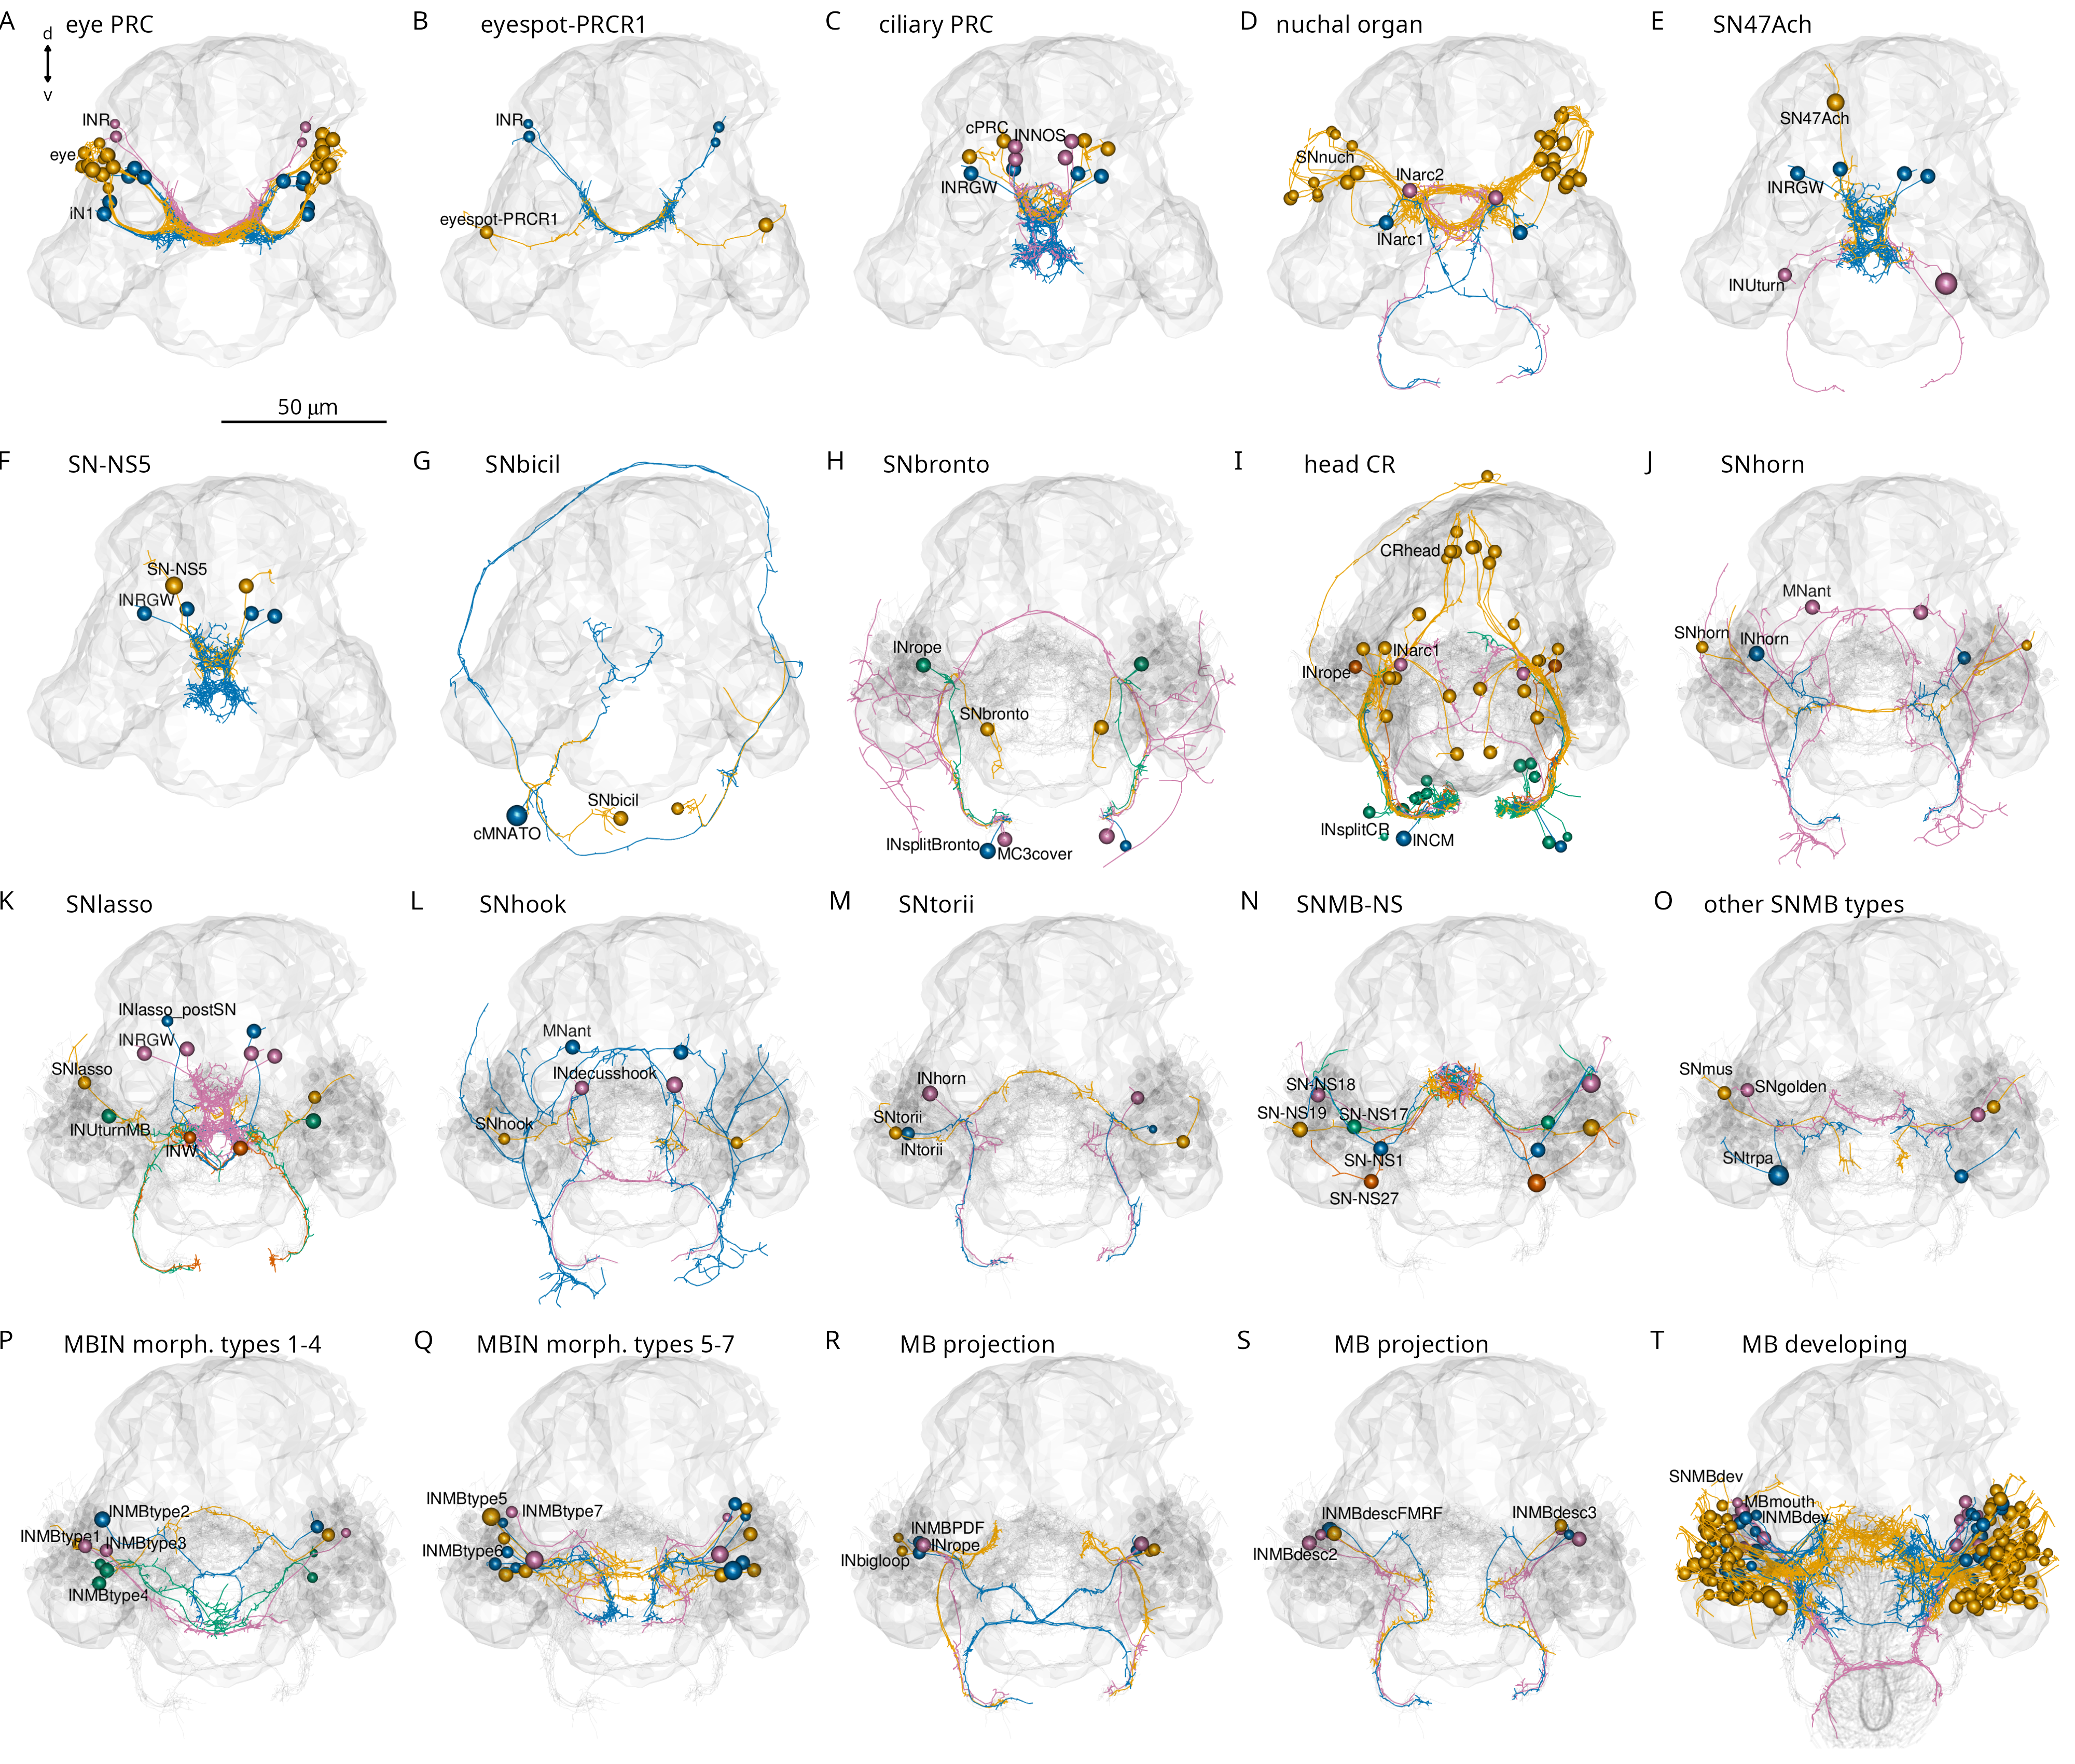
\includegraphics[width=1\textwidth,height=\textheight]{Figures/Figure6_fig_suppl1.png}

}

\caption{\textbf{Figure 6---figure supplement 1. Head cell types and
circuits. } (A) The adult eye photoreceptor cells (PRC) with their
direct IN1 and INR synaptic targets. (B) The eyespot PRCR1 cells with
their INR targets. (C) The ciliary PRCs with their INRGWa and INNOS
targets. (D) The nuchal organ sensory neurons with their INarc1 and
INarc2 targets. (E) The asymmetric SN47Ach neuron with its INRGWa and
INUturn targets. (F) The SN-NS5 neurons with their INRGWa targets. (G)
The SNbicil neuron with their cMNATO target. (H) The SNbronto neurons
with their INrope, INsplitBronto (segment 1) and MC3cover (segment 1)
targets. (I) The head collar receptor neurons (CR) with their INarc1,
INrope, INCM (segment 1) and INsplitCR (trunk) targets. (J) The SNhorn
neurons with their INhorn and MNant targets. (K) The SNlasso neurons
with their diverse interneuron targets. (L) The SNhook neurons with
their INdecusshook and MNant targets. (M) The SNtorii neurons with their
INtorii and INhorn targets. (N) Sensory cells of the mushroom body
(SNMB-NS) that project into the neurosecretory plexus. (O) The SNmus,
SNgolden and SNtrpa sensory neurons of the mushroom body. (P) Mushroom
body interneurons, morphological types 1-4. (Q) Mushroom body
interneurons, morphological types 5-7. (R) The INrope, INbigloop and
INMBPDF mushroom body projection neurons. (S) The INMBdescFMRF,
INMBdesc2 and INMBdesc3 mushroom body projection neurons. (T) Developing
mushroom body neurons.}

\end{figure}%

\begin{figure}[H]

{\centering 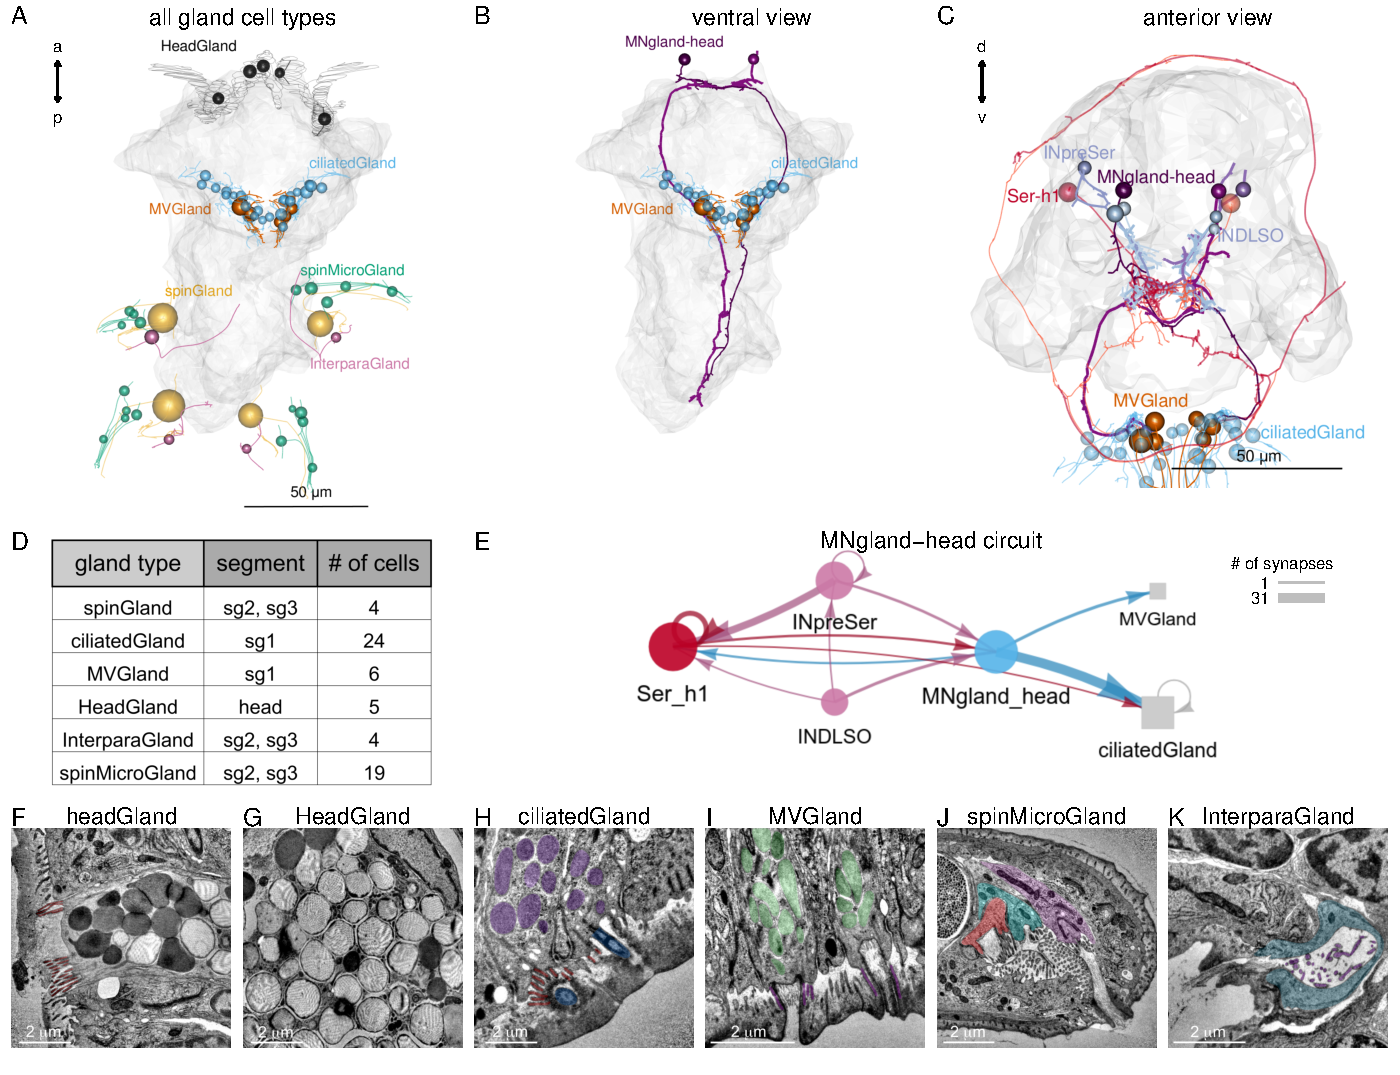
\includegraphics[width=1\textwidth,height=\textheight]{Figures/Figure7_fig_suppl1.png}

}

\caption{\textbf{Figure 7---figure supplement 1. Gland cells and their
innervation.} (A) Morphological rendering of all gland cells classified
into six types. Gland cell-types differ in their position, size,
ultrastructure and innervation. These cells have long projections, but
we could not identify synaptic inputs to them. (B) Morphological
rendering of MNgland-head motoneurons and their MVGland and
ciliatedGland target cells in the first segment, ventral view. (C)
MNgland-head motoneurons, their presynaptic partners and gland targets,
anterior view. (D) Summary of gland cell types, their segmental location
and segmental positions. (E) Circuit diagram of MNgland-head neurons.
(F-G) TEM images of headGland cells. In the ventral head, there are five
large headGland cells. These cells are filled with large (diameter=1.4
µm, stdev=0.28 N=36) secretory vesicles and have no presynaptic
partners. (H) TEM image of the secretory pore of a ciliatedGland cell
with a microvillar collar and a stiff cilium penetrating the cuticle.
The ciliatedGland cells are part of a ventral girdle of gland cells in
the first segment, together with the MVGland cells. (I) TEM image of the
secretory pore of a microvillar MVGland cell with a broader microvillar
secretory pore and no cilium. (J) TEM image of the secretory pore of a
spinMicroGland, close to the pore of the large spinGlands.
SpinMicroGland cells have microvilli and secrete through a narrow tunnel
in the cuticle. They have no synaptic inputs. (K) TEM image of the
secretory pore of an interparaGland. These cells have a small
microvillar secretory pore opening in the cuticle between the neuro- and
notopodia. The interparaGlands also lack synaptic inputs. Figure
7---figure supplement 1---source data 1. Source data for MNgland-head
connectivity.}

\end{figure}%

\begin{figure}[H]

{\centering \includegraphics[width=1\textwidth,height=\textheight]{Figures/Figure7_fig_suppl2.png}

}

\caption{\textbf{Figure 7---figure supplement 2. Metrics of head cell
types.} (A) Number of postsynaptic cell-type partners of head neuronal
cell types. (B) Number of presynaptic cell-type partners of head
neuronal cell types. (C) Head cell-types ranked by weighted degree. (D)
Head cell-types ranked by pagerank centrality. (E) Head cell-types
ranked by betweenness centrality. (F) Head cell-types ranked by square
root of authority centrality. Only the top 28 cell types are shown.
Source data are the same as for Figure 4.}

\end{figure}%

\begin{figure}[H]

{\centering \includegraphics[width=1\textwidth,height=\textheight]{Figures/Figure7_fig_suppl3.png}

}

\caption{\textbf{Figure 7---figure supplement 3. Number of partners of
head sensory and interneuron types.} (A) Number of postsynaptic
interneuron cell-type partners of head sensory cell types. (B) Number of
presynaptic head sensory cell-type partners of head interneurons and
motoneurons. (C) Number of postsynaptic head interneuron cell-type
partners of head interneurons. (D) Number of presynaptic head
interneuron cell-type partners of head interneurons. (E) Morphological
rendering of hCR neurons and their postsynaptic interneuron partners.
(F) INRGWa neurons and their presynaptic sensory neuron partners. (G)
INRGWa neurons and their postsynaptic interneuron partners. (H) INW
neurons and their postsynaptic interneuron partners. In (A-D) only cell
types with 2 or more partners are shown. Each partner has at least two
synapses. Source data are the same as for Figure 4.}

\end{figure}%

\begin{figure}[H]

{\centering \includegraphics[width=1\textwidth,height=\textheight]{Figures/Figure9_fig_suppl1.png}

}

\caption{\textbf{Figure 9---figure supplement 1. The mushroom body
circuit with different subcircuits highlighted.} (A) Sensory cells with
inputs into the mushroom body and their direct pre- and postsynaptic
partners. (B) Mushroom-body-intrinsic sensory neurons and their direct
pre- and postsynaptic partners. (C) Mushroom-body-intrinsic interneurons
and their direct pre- and postsynaptic partners. (D) Mushroom body
projection interneurons and their direct pre- and postsynaptic
partners.}

\end{figure}%

\begin{figure}[H]

{\centering \includegraphics[width=1\textwidth,height=\textheight]{Figures/Figure9_fig_Suppl2.png}

}

\caption{\textbf{Figure 9---figure supplement 2. Left-right symmetry of
mushroom body cell types and their wiring.} (A-B) Average Sholl diagrams
for mushroom body cell types on the left and right side. (C-D)
Connectivity matrix of mushroom body cell types on the left and the
right side. Figure 9---figure supplement 2---source data 1. Source data
for panel A. Figure 9---figure supplement 2---source data 2. Source data
for panel B. Figure 9---figure supplement 2---source data 3. Source data
for panel C. Figure 9---figure supplement 2---source data 4. Source data
for panel D.}

\end{figure}%

\begin{figure}[H]

{\centering \includegraphics[width=1\textwidth,height=\textheight]{Figures/Figure10_fig_suppl1.png}

}

\caption{\textbf{Figure 10---figure supplement 1. Head descending and
decussating neurons.} (A) Morphological rendering of the neurites of
head desending (blue) and decussationg (yellow) neurons. (B) Names of
head descending and decussationg cell types. (C) Incoming synapses on
head descending and decussating neurons. (D) Outgoing synapses of head
descending and decussating neurons. (E) Postsynaptic targets of head
descending and decussating neurons. (F) Distribution of the neurites of
head descending and decussating neurons in the VNC. Cross section at the
position of the thin line in (E). (G) Neurites of the postsynaptic
targets of head descending and decussating neurons in the VNC. Cross
section at the position of the thin line in (E). (H-I) Incoming (red)
and outgoing (blue) synapses of head decussating neurons in anterior (H)
and ventral (I) view. (J) Mean radial density of incoming and outgoing
synapses in head decussating neurons. (K-L) Incoming (red) and outgoing
(blue) synapses of head descending neurons in anterior (K) and ventral
(L) view. (M) Mean radial density of incoming and outgoing synapses in
head descending neurons. Figure 10---figure supplement 1---source data
1. Source data for panels (J, M).}

\end{figure}%

\begin{figure}[H]

{\centering \includegraphics[width=1\textwidth,height=\textheight]{Figures/Figure10_fig_suppl2.png}

}

\caption{\textbf{Figure 10---figure supplement 2. Head-trunk
connectivity.} Distribution across segments of trunk targets of head
neurons ordered by the number of head to trunk synapses (top 50 neurons
shown).}

\end{figure}%

\begin{figure}[H]

{\centering \includegraphics[width=1\textwidth,height=\textheight]{Figures/Figure10_fig_suppl3.png}

}

\caption{\textbf{Figure 10---figure supplement 3. Connectivity of
head-trunk cell groups.} (A) Grouped connectivity matrix between head
and trunk sensory (SN), inter- (IN), motoneurons (MN) and effectors. (B)
Sankey information-flow network of head-trunk cell groups, as in A. Only
connections with \textgreater20 synapses are shown. Line width is
proportional to the square root of synapse number. Figure 10---figure
supplement 3---source data 1. The source data matrix as a csv file.}

\end{figure}%

\begin{figure}[H]

{\centering \includegraphics[width=1\textwidth,height=\textheight]{Figures/Figure10_fig_suppl4.png}

}

\caption{\textbf{Figure 10---figure supplement 4. Connectivity of
left-right cell groups.} (A) Grouped connectivity matrix between left
and right sensory (SN), inter- (IN), motoneurons (MN) and effectors. (B)
Sankey information-flow network of left-right cell groups, as in A. Only
connections with \textgreater20 synapses are shown. Line width is
proportional to the square root of synapse number. Figure 10---figure
supplement 4---source data 1. The source data matrix as a csv file.}

\end{figure}%

\begin{figure}[H]

{\centering \includegraphics[width=1\textwidth,height=\textheight]{Figures/Figure11_fig_suppl1.png}

}

\caption{\textbf{Figure 11---figure supplement 1. Connectivity matrix of
cell categories across the six body regions. } Source data are the same
as for Figure 11 panel C}

\end{figure}%

\begin{figure}[H]

{\centering \includegraphics[width=1\textwidth,height=\textheight]{Figures/Figure12_fig_suppl1.png}

}

\caption{\textbf{Figure 12---figure supplement 1. Statistics of trunk
cell types. } (A) Histogram of the number of cells per trunk cell-type.
(B) Histogram of the number of presynaptic cell-type partners of trunk
neurons. (C) Histogram of the number of postsynaptice cell-type partners
of trunk neurons}

\end{figure}%

\begin{figure}[H]

{\centering \includegraphics[width=1\textwidth,height=\textheight]{Figures/Figure12_fig_suppl2.png}

}

\caption{\textbf{Figure 12---figure supplement 2. Partners and
centrality measures of trunk cell types.} (A) Number of postsynaptic
cell-type partners of trunk neuronal cell types (\textgreater4
synapses). (B) Number of presynaptic neuron types for different trunk
cell types. (C) Trunk cell-types ranked by weighted degree. (D) Trunk
cell-types ranked by pagerank centrality. (E) Trunk cell-types ranked by
betweenness centrality. (F) Trunk cell-types ranked by authority. In
(D-F) only the top 28 cell types are shown.}

\end{figure}%

\begin{figure}[H]

{\centering \includegraphics[width=1\textwidth,height=\textheight]{Figures/Figure12_fig_suppl3.png}

}

\caption{\textbf{Figure 12---figure supplement 3. Segment-specific cell
types. } Morphological rendering of segment-specific neuron types in
different trunk segments. i) SNstiff neurons of segment 0. ii-xv) Cell
types specific to segment 1. xvi-xxiv) Cell types specific to segment 2.
xxv-xxvi) Cell types specific to segment 3. xxvii-xxxv) Cell types
specific to the pygidium. All panels show a ventral view. The yolk
outline is shown for reference. All other cells in the same segment as
the rendered neurons are also shown for each panel for reference.}

\end{figure}%

\begin{figure}[H]

{\centering \includegraphics[width=1\textwidth,height=\textheight]{Figures/Figure14_fig_suppl1.png}

}

\caption{\textbf{Figure 14---figure supplement 1. All cell types within
the mechanosensory girdle. } (i-xi) Morphological renderings of all
neuron types that are part of the mechanosensory girdle.}

\end{figure}%

\begin{figure}[H]

{\centering \includegraphics[width=1\textwidth,height=\textheight]{Figures/Figure14_fig_suppl2.png}

}

\caption{\textbf{Figure 14---figure supplement 2. Cross-section of the
ventral nerve cord. } Axons from the from the mechanosensory girdle are
highlighted.}

\end{figure}%

\begin{figure}[H]

{\centering \includegraphics[width=1\textwidth,height=\textheight]{Figures/Figure16_fig_suppl1.png}

}

\caption{\textbf{Figure 16---figure supplement 1. Connectivity of
mechanosensory neurons. } Grouped synaptic connectivity matrix of
mechanosensory neurons and their postsynaptic targets. Figure
16---figure supplement 1---source data 1. The connectivity matrix in csv
format}

\end{figure}%

\section{Videos}\label{videos}

Video 1. Video 2. Video 3. Video 4. Video 5.

\hfill\break

\section{References}\label{references}

\hfill\break

\phantomsection\label{refs}
\begin{CSLReferences}{1}{0}
\bibitem[\citeproctext]{ref-Achim2015}
Achim K, Pettit J-B, Saraiva LR, Gavriouchkina D, Larsson T, Arendt D,
Marioni JC. 2015. High-throughput spatial mapping of single-cell RNA-seq
data to tissue of origin. \emph{Nature Biotechnology}
\textbf{33}:503--509.
doi:\href{https://doi.org/10.1038/nbt.3209}{10.1038/nbt.3209}

\bibitem[\citeproctext]{ref-allaire2017package}
Allaire J, Ellis P, Gandrud C, Kuo K, Lewis B, Owen J, Russell K, Rogers
J, Sese C, Yetman C, others. 2017. Package {``networkD3.''} \emph{D3
JavaScript network graphs from R}.

\bibitem[\citeproctext]{ref-almende2019package}
Almende B, Thieurmel B, Robert T. 2019. Package {``visnetwork.''}
\emph{Network Visualization Using {``vis js''} Library, Version}
\textbf{2}.

\bibitem[\citeproctext]{ref-arendt2008evolution}
Arendt D. 2008. The evolution of cell types in animals: Emerging
principles from molecular studies. \emph{Nature Reviews Genetics}
\textbf{9}:868--882.

\bibitem[\citeproctext]{ref-arendt2021conserved}
Arendt D, Urzainqui IQ, Vergara HM. 2021. The conserved core of the
nereid brain: Circular CNS, apical nervous system and lhx6-arx-dlx
neurons. \emph{Current Opinion in Neurobiology} \textbf{71}:178--187.

\bibitem[\citeproctext]{ref-balfour1881treatise}
Balfour FM. 1881. A treatise on comparative embryology: Vol. II.
Macmillan \& Co.

\bibitem[\citeproctext]{ref-bastian2009gephi}
Bastian M, Heymann S, Jacomy M. 2009. Gephi: An open source software for
exploring and manipulating networksProceedings of the International AAAI
Conference on Web and Social Media. pp. 361--362.

\bibitem[\citeproctext]{ref-bates2020natverse}
Bates AS, Manton JD, Jagannathan SR, Costa M, Schlegel P, Rohlfing T,
Jefferis GS. 2020. The natverse, a versatile toolbox for combining and
analysing neuroanatomical data. \emph{Elife} \textbf{9}:e53350.

\bibitem[\citeproctext]{ref-Bentley2016}
Bentley B, Branicky R, Barnes CL, Chew YL, Yemini E, Bullmore ET, Vértes
PE, Schafer WR. 2016. The Multilayer Connectome of Caenorhabditis
elegans. \emph{PLOS Computational Biology} \textbf{12}:e1005283.
doi:\href{https://doi.org/10.1371/journal.pcbi.1005283}{10.1371/journal.pcbi.1005283}

\bibitem[\citeproctext]{ref-bezares-calderon2018}
Bezares-Calderón LA, Berger J, Jasek S, Verasztó C, Mendes S, Gühmann M,
Almeda R, Shahidi R, Jékely G. 2018. Neural circuitry of a
polycystin-mediated hydrodynamic startle response for predator
avoidance. \emph{eLife} \textbf{7}.
doi:\href{https://doi.org/10.7554/elife.36262}{10.7554/elife.36262}

\bibitem[\citeproctext]{ref-bidel2023connectomics}
Bidel F, Meirovitch Y, Schalek RL, Lu X, Pavarino EC, Yang F, Peleg A,
Wu Y, Shomrat T, Berger DR, others. 2023. Connectomics of the octopus
vulgaris vertical lobe provides insight into conserved and novel
principles of a memory acquisition network. \emph{Elife}
\textbf{12}:e84257.

\bibitem[\citeproctext]{ref-brunet2016evolutionary}
Brunet T, Fischer AH, Steinmetz PR, Lauri A, Bertucci P, Arendt D. 2016.
The evolutionary origin of bilaterian smooth and striated myocytes.
\emph{Elife} \textbf{5}:e19607.

\bibitem[\citeproctext]{ref-Bezares2023barotaxis}
Calderón LAB, Shahidi R, Jékely G. 2023. Mechanism of barotaxis in
marine zooplankton. \emph{bioRxiv}.
doi:\href{https://doi.org/10.1101/2023.02.28.530398}{10.1101/2023.02.28.530398}

\bibitem[\citeproctext]{ref-cardona2012}
Cardona A, Saalfeld S, Schindelin J, Arganda-Carreras I, Preibisch S,
Longair M, Tomancak P, Hartenstein V, Douglas RJ. 2012. TrakEM2 Software
for Neural Circuit Reconstruction. \emph{PLoS ONE} \textbf{7}:e38011.
doi:\href{https://doi.org/10.1371/journal.pone.0038011}{10.1371/journal.pone.0038011}

\bibitem[\citeproctext]{ref-carreira2018mdn}
Carreira-Rosario A, Zarin AA, Clark MQ, Manning L, Fetter RD, Cardona A,
Doe CQ. 2018. MDN brain descending neurons coordinately activate
backward and inhibit forward locomotion. \emph{Elife} \textbf{7}:e38554.

\bibitem[\citeproctext]{ref-Conzelmann2011}
Conzelmann M, Offenburger S-L, Asadulina A, Keller T, Münch TA, Jékely
G. 2011. Neuropeptides regulate swimming depth of {\emph{Platynereis}}
larvae. \emph{Proceedings of the National Academy of Sciences}
\textbf{108}.
doi:\href{https://doi.org/10.1073/pnas.1109085108}{10.1073/pnas.1109085108}

\bibitem[\citeproctext]{ref-Conzelmann2013}
Conzelmann M, Williams EA, Tunaru S, Randel N, Shahidi R, Asadulina A,
Berger J, Offermanns S, Jékely G. 2013. Conserved MIP
receptor{\textendash}ligand pair regulates {\emph{Platynereis}} larval
settlement. \emph{Proceedings of the National Academy of Sciences}
\textbf{110}:8224--8229.
doi:\href{https://doi.org/10.1073/pnas.1220285110}{10.1073/pnas.1220285110}

\bibitem[\citeproctext]{ref-cook2019whole}
Cook SJ, Jarrell TA, Brittin CA, Wang Y, Bloniarz AE, Yakovlev MA,
Nguyen KC, Tang LT-H, Bayer EA, Duerr JS, others. 2019. Whole-animal
connectomes of both caenorhabditis elegans sexes. \emph{Nature}
\textbf{571}:63--71.

\bibitem[\citeproctext]{ref-csardi2006igraph}
Csardi G, Nepusz T, others. 2006. The igraph software package for
complex network research. \emph{InterJournal, complex systems}
\textbf{1695}:1--9.

\bibitem[\citeproctext]{ref-Deng2019}
Deng B, Li Q, Liu X, Cao Y, Li B, Qian Y, Xu R, Mao R, Zhou E, Zhang W,
Huang J, Rao Y. 2019. Chemoconnectomics: Mapping Chemical Transmission
in Drosophila. \emph{Neuron} \textbf{101}:876--893.e4.
doi:\href{https://doi.org/10.1016/j.neuron.2019.01.045}{10.1016/j.neuron.2019.01.045}

\bibitem[\citeproctext]{ref-dorsett1964sensory}
Dorsett D. 1964. The sensory and motor innervation of nereis.
\emph{Proceedings of the Royal Society of London Series B Biological
Sciences} \textbf{159}:652--667.

\bibitem[\citeproctext]{ref-franconville2018building}
Franconville R, Beron C, Jayaraman V. 2018. Building a functional
connectome of the drosophila central complex. \emph{Elife}
\textbf{7}:e37017.

\bibitem[\citeproctext]{ref-he2019direction}
He L, Gulyanon S, Skanata MM, Karagyozov D, Heckscher ES, Krieg M,
Tsechpenakis G, Gershow M, Tracey WD. 2019. Direction selectivity in
drosophila proprioceptors requires the mechanosensory channel tmc.
\emph{Current Biology} \textbf{29}:945--956.

\bibitem[\citeproctext]{ref-Helmstaedter2013}
Helmstaedter M. 2013. Cellular-resolution connectomics: challenges of
dense neural circuit reconstruction. \emph{Nature Methods}
\textbf{10}:501--507.
doi:\href{https://doi.org/10.1038/nmeth.2476}{10.1038/nmeth.2476}

\bibitem[\citeproctext]{ref-horridge1963proprioceptors}
Horridge GA. 1963. Proprioceptors, bristle receptors, efferent sensory
impulses, neurofibrils and number of axons in the parapodial nerve of
the polychaete harmotho{ë}. \emph{Proceedings of the Royal Society of
London Series B Biological Sciences} \textbf{157}:199--222.

\bibitem[\citeproctext]{ref-jasek2022}
Jasek S, Verasztó C, Brodrick E, Shahidi R, Kazimiers T, Kerbl A, Jékely
G. 2022. Desmosomal connectomics of all somatic muscles in an annelid
larva. \emph{eLife} \textbf{11}.
doi:\href{https://doi.org/10.7554/elife.71231}{10.7554/elife.71231}

\bibitem[\citeproctext]{ref-jekely_2024_10825371}
Jékely G, Jasek S, Gühmann M, Bezares-Calderón LA, Williams EA, Shahidi
R. 2024. {Code documentation for the Jekely et al. three- day-old
Platynereis larva connectome paper}.
doi:\href{https://doi.org/10.5281/zenodo.10825371}{10.5281/zenodo.10825371}

\bibitem[\citeproctext]{ref-jokura2023nitric}
Jokura K, Ueda N, Guehmann M, Yanez-Guerra LA, Slowinski P, Wedgwood KC,
Jekely G. 2023. Nitric oxide feedback to ciliary photoreceptor cells
gates a UV avoidance circuit. \emph{bioRxiv} 2023--08.

\bibitem[\citeproctext]{ref-kebschull2020cerebellar}
Kebschull JM, Richman EB, Ringach N, Friedmann D, Albarran E, Kolluru
SS, Jones RC, Allen WE, Wang Y, Cho SW, others. 2020. Cerebellar nuclei
evolved by repeatedly duplicating a conserved cell-type set.
\emph{Science} \textbf{370}:eabd5059.

\bibitem[\citeproctext]{ref-miroschnikow2018convergence}
Miroschnikow A, Schlegel P, Schoofs A, Hueckesfeld S, Li F,
Schneider-Mizell CM, Fetter RD, Truman JW, Cardona A, Pankratz MJ. 2018.
Convergence of monosynaptic and polysynaptic sensory paths onto common
motor outputs in a drosophila feeding connectome. \emph{Elife}
\textbf{7}:e40247.

\bibitem[\citeproctext]{ref-Morgan2013}
Morgan JL, Lichtman JW. 2013. Why not connectomics? \emph{Nature
Methods} \textbf{10}:494--500.
doi:\href{https://doi.org/10.1038/nmeth.2480}{10.1038/nmeth.2480}

\bibitem[\citeproctext]{ref-nielsen2005larval}
Nielsen C. 2005. Larval and adult brains 1. \emph{Evolution \&
development} \textbf{7}:483--489.

\bibitem[\citeproctext]{ref-nielsen2018evolution}
Nielsen C, Brunet T, Arendt D. 2018. Evolution of the bilaterian mouth
and anus. \emph{Nature ecology \& evolution} \textbf{2}:1358--1376.

\bibitem[\citeproctext]{ref-ohyama2015multilevel}
Ohyama T, Schneider-Mizell CM, Fetter RD, Aleman JV, Franconville R,
Rivera-Alba M, Mensh BD, Branson KM, Simpson JH, Truman JW, others.
2015. A multilevel multimodal circuit enhances action selection in
drosophila. \emph{Nature} \textbf{520}:633--639.

\bibitem[\citeproctext]{ref-parry2015cambrian}
Parry L, Vinther J, Edgecombe GD. 2015. Cambrian stem-group annelids and
a metameric origin of the annelid head. \emph{Biology letters}
\textbf{11}:20150763.

\bibitem[\citeproctext]{ref-RStudio}
Posit team. 2023. \href{http://www.posit.co/}{RStudio: Integrated
development environment for r}. Boston, MA: Posit Software, PBC.

\bibitem[\citeproctext]{ref-randel2014neuronal}
Randel N, Asadulina A, Bezares-Calderón LA, Verasztó C, Williams EA,
Conzelmann M, Shahidi R, Jékely G. 2014. Neuronal connectome of a
sensory-motor circuit for visual navigation. \emph{elife}
\textbf{3}:e02730.

\bibitem[\citeproctext]{ref-Randel2015}
Randel N, Shahidi R, Verasztó C, Bezares-Calderón LA, Schmidt S, Jékely
G. 2015. Inter-individual stereotypy of the Platynereis larval visual
connectome. \emph{eLife} \textbf{4}.
doi:\href{https://doi.org/10.7554/elife.08069}{10.7554/elife.08069}

\bibitem[\citeproctext]{ref-ryan2016cns}
Ryan K, Lu Z, Meinertzhagen IA. 2016. The CNS connectome of a tadpole
larva of ciona intestinalis (l.) highlights sidedness in the brain of a
chordate sibling. \emph{Elife} \textbf{5}:e16962.

\bibitem[\citeproctext]{ref-Saalfeld2009}
Saalfeld S, Cardona A, Hartenstein V, Tomančák P. 2009. CATMAID:
collaborative annotation toolkit for massive amounts of image data.
\emph{Bioinformatics} \textbf{25}:1984--1986.
doi:\href{https://doi.org/10.1093/bioinformatics/btp266}{10.1093/bioinformatics/btp266}

\bibitem[\citeproctext]{ref-Schlegel2017}
Schlegel P, Costa M, Jefferis GS. 2017. Learning from connectomics on
the fly. \emph{Current Opinion in Insect Science} \textbf{24}:96--105.
doi:\href{https://doi.org/10.1016/j.cois.2017.09.011}{10.1016/j.cois.2017.09.011}

\bibitem[\citeproctext]{ref-Schneider-Mizell2016}
Schneider-Mizell CM, Gerhard S, Longair M, Kazimiers T, Li F, Zwart MF,
Champion A, Midgley FM, Fetter RD, Saalfeld S, Cardona A. 2016.
Quantitative neuroanatomy for connectomics in Drosophila. \emph{eLife}
\textbf{5}.
doi:\href{https://doi.org/10.7554/elife.12059}{10.7554/elife.12059}

\bibitem[\citeproctext]{ref-schorb2019software}
Schorb M, Haberbosch I, Hagen WJ, Schwab Y, Mastronarde DN. 2019.
Software tools for automated transmission electron microscopy.
\emph{Nature methods} \textbf{16}:471--477.

\bibitem[\citeproctext]{ref-sedgwick1884origin}
Sedgwick A. 1884. On the origin of metameric segmentation and some other
morphological questions. \emph{Journal of Cell Science}
\textbf{2}:43--82.

\bibitem[\citeproctext]{ref-shahidi2015serial}
Shahidi R, Williams EA, Conzelmann M, Asadulina A, Veraszto C, Jasek S,
Bezares-Calderon LA, Jekely G. 2015. A serial multiplex immunogold
labeling method for identifying peptidergic neurons in connectomes.
\emph{Elife} \textbf{4}:e11147.

\bibitem[\citeproctext]{ref-shomrat2011alternative}
Shomrat T, Graindorge N, Bellanger C, Fiorito G, Loewenstein Y, Hochner
B. 2011. Alternative sites of synaptic plasticity in two homologous
{``fan-out fan-in''} learning and memory networks. \emph{Current
biology} \textbf{21}:1773--1782.

\bibitem[\citeproctext]{ref-singla1975statocysts}
Singla C. 1975. Statocysts of hydromedusae. \emph{Cell and Tissue
Research} \textbf{158}:391--407.

\bibitem[\citeproctext]{ref-starunov2015metameric}
Starunov VV, Dray N, Belikova EV, Kerner P, Vervoort M, Balavoine G.
2015. A metameric origin for the annelid pygidium? \emph{BMC
Evolutionary Biology} \textbf{15}:1--17.

\bibitem[\citeproctext]{ref-steinmetz2011segmental}
Steinmetz PR, Kostyuchenko RP, Fischer A, Arendt D. 2011. The segmental
pattern of otx, gbx, and hox genes in the annelid platynereis dumerilii.
\emph{Evolution \& development} \textbf{13}:72--79.

\bibitem[\citeproctext]{ref-tomer2010profiling}
Tomer R, Denes AS, Tessmar-Raible K, Arendt D. 2010. Profiling by image
registration reveals common origin of annelid mushroom bodies and
vertebrate pallium. \emph{Cell} \textbf{142}:800--809.

\bibitem[\citeproctext]{ref-tosches2017developmental}
Tosches MA. 2017. Developmental and genetic mechanisms of neural circuit
evolution. \emph{Developmental biology} \textbf{431}:16--25.

\bibitem[\citeproctext]{ref-traag2019louvain}
Traag VA, Waltman L, Van Eck NJ. 2019. From louvain to leiden:
Guaranteeing well-connected communities. \emph{Scientific reports}
\textbf{9}:5233.

\bibitem[\citeproctext]{ref-vaadia2019}
Vaadia RD, Li W, Voleti V, Singhania A, Hillman EM, Grueber WB. 2019.
Characterization of proprioceptive system dynamics in behaving
drosophila larvae using high-speed volumetric microscopy. \emph{Current
Biology} \textbf{29}:935--944.

\bibitem[\citeproctext]{ref-veraszto2018}
Verasztó C, Gühmann M, Jia H, Rajan VBV, Bezares-Calderón LA,
Piñeiro-Lopez C, Randel N, Shahidi R, Michiels NK, Yokoyama S,
Tessmar-Raible K, Jékely G. 2018. Ciliary and rhabdomeric
photoreceptor-cell circuits form a spectral depth gauge in marine
zooplankton. \emph{eLife} \textbf{7}.
doi:\href{https://doi.org/10.7554/elife.36440}{10.7554/elife.36440}

\bibitem[\citeproctext]{ref-veraszto2020}
Verasztó C, Jasek S, Gühmann M, Shahidi R, Ueda N, Beard JD, Mendes S,
Heinz K, Bezares-Calderón LA, Williams E, Jékely G. 2020.
\href{http://dx.doi.org/10.1101/2020.08.21.260984}{Whole-animal
connectome and cell-type complement of the three-segmented
{\emph{Platynereis dumerilii}} larva}.

\bibitem[\citeproctext]{ref-veraszto2017}
Verasztó C, Ueda N, Bezares-Calderón LA, Panzera A, Williams EA, Shahidi
R, Jékely G. 2017. Ciliomotor circuitry underlying whole-body
coordination of ciliary activity in the Platynereis larva. \emph{eLife}
\textbf{6}.
doi:\href{https://doi.org/10.7554/elife.26000}{10.7554/elife.26000}

\bibitem[\citeproctext]{ref-vergara2017whole}
Vergara HM, Bertucci PY, Hantz P, Tosches MA, Achim K, Vopalensky P,
Arendt D. 2017. Whole-organism cellular gene-expression atlas reveals
conserved cell types in the ventral nerve cord of platynereis dumerilii.
\emph{Proceedings of the National Academy of Sciences}
\textbf{114}:5878--5885.

\bibitem[\citeproctext]{ref-Vergara2021}
Vergara HM, Pape C, Meechan KI, Zinchenko V, Genoud C, Wanner AA, Mutemi
KN, Titze B, Templin RM, Bertucci PY, Simakov O, Dürichen W, Machado P,
Savage EL, Schermelleh L, Schwab Y, Friedrich RW, Kreshuk A, Tischer C,
Arendt D. 2021. Whole-body integration of gene expression and
single-cell morphology. \emph{Cell} \textbf{184}:4819--4837.e22.
doi:\href{https://doi.org/10.1016/j.cell.2021.07.017}{10.1016/j.cell.2021.07.017}

\bibitem[\citeproctext]{ref-white1986structure}
White JG, Southgate E, Thomson JN, Brenner S, others. 1986. The
structure of the nervous system of the nematode caenorhabditis elegans.
\emph{Philos Trans R Soc Lond B Biol Sci} \textbf{314}:1--340.

\bibitem[\citeproctext]{ref-wickham2019welcome}
Wickham H, Averick M, Bryan J, Chang W, McGowan LD, François R,
Grolemund G, Hayes A, Henry L, Hester J, others. 2019. Welcome to the
tidyverse. \emph{Journal of open source software} \textbf{4}:1686.

\bibitem[\citeproctext]{ref-wickham2016package}
Wickham H, Chang W, Wickham MH. 2016. Package {``ggplot2.''}
\emph{Create elegant data visualisations using the grammar of graphics
Version} \textbf{2}:1--189.

\bibitem[\citeproctext]{ref-williams2015myoinhibitory}
Williams EA, Conzelmann M, Jékely G. 2015. Myoinhibitory peptide
regulates feeding in the marine annelid platynereis. \emph{Frontiers in
zoology} \textbf{12}:1--16.

\bibitem[\citeproctext]{ref-williams2017}
Williams EA, Verasztó C, Jasek S, Conzelmann M, Shahidi R, Bauknecht P,
Mirabeau O, Jékely G. 2017. Synaptic and peptidergic connectome of a
neurosecretory center in the annelid brain. \emph{eLife} \textbf{6}.
doi:\href{https://doi.org/10.7554/elife.26349}{10.7554/elife.26349}

\bibitem[\citeproctext]{ref-winding2023connectome}
Winding M, Pedigo BD, Barnes CL, Patsolic HG, Park Y, Kazimiers T,
Fushiki A, Andrade IV, Khandelwal A, Valdes-Aleman J, others. 2023. The
connectome of an insect brain. \emph{Science} \textbf{379}:eadd9330.

\bibitem[\citeproctext]{ref-zarin2019multilayer}
Zarin AA, Mark B, Cardona A, Litwin-Kumar A, Doe CQ. 2019. A multilayer
circuit architecture for the generation of distinct locomotor behaviors
in drosophila. \emph{Elife} \textbf{8}:e51781.

\bibitem[\citeproctext]{ref-zheng2018complete}
Zheng Z, Lauritzen JS, Perlman E, Robinson CG, Nichols M, Milkie D,
Torrens O, Price J, Fisher CB, Sharifi N, others. 2018. A complete
electron microscopy volume of the brain of adult drosophila
melanogaster. \emph{Cell} \textbf{174}:730--743.

\end{CSLReferences}



\end{document}
